

\section{Выбор средств программной реализации}

\subsection{Язык программирования}
В качестве языка программирования был выбран Python 3\cite{python_doc}, по следующим причинам.
\begin{itemize}
	\item Поддержка ООП, требуемого для архитектурного шаблона MVC.
	\item Наличие опыта работы с данным языком.
	\item Данный язык является популярным в разработке web-приложений, поэтому он обладает большим количеством web-фреймворков и библиотек для доступа к СУБД.
\end{itemize}

\subsection{СУБД и ORM}
Наиболее популярными реляционными СУБД являются Oracle, MySQL и PostgreSQL\cite{dbm_source}. Их сравнение\cite{dbm_source2} можно свести в таблицу \ref{dms_table2}

\begin{center}
\begin{longtable}[h]{| p{2.4cm} | p{6.6cm} | p{6.6cm} |}
	\caption{Сравнение реляционных СУБД} \label{dms_table2} \\
 	\hline 
	\multicolumn{1}{|c|}{\textbf{СУБД}} &
	\multicolumn{1}{c|}{\textbf{Преимущества}} &
	\multicolumn{1}{c|}{\textbf{Недостатки}} \\
	\hline
	\endfirsthead
	
	\multicolumn{3}{c}%
	{{\tablename\ \thetable{} -- продолжение}} \\
 	\hline 
	\multicolumn{1}{|c|}{\textbf{СУБД}} &
	\multicolumn{1}{c|}{\textbf{Преимущества}} &
	\multicolumn{1}{c|}{\textbf{Недостатки}} \\
	\hline
	\endhead
	
	\hline \multicolumn{3}{|r|}{{Продолжение на следующей странице}} \\ \hline
	\endfoot
	
	\hline
	\endlastfoot
	
	\hline
	Oracle		&	+ надёжность системы	& -	конечная стоимость СУБД	\\ 
	&	+ поддержка современности функционала	& - высокие системные требования \\ 
	\hline
	
	MySQL	&	+ прост в установке и использовании	& -	проблемы с надёжностью	\\ 
	&	+ производительность и надёжность	& - не полная поддержка SQL \\ 
	&	+ широкий базовый функционал & \\
	\hline
	
	PostgreSQL	&	+ лёгкая масштабируемость	& -	низкая скорость выполнения пакетных операций	\\ 
	&	+ открытость ПО	& - сложности поиска хостинга \\ 
	&	+ поддержка текстовых форматов (в т.ч. json) & \\
\end{longtable}
\end{center}

Наиболее подходящим для небольших организаций, которые являются целевыми для разрабатываемой программы, является PostgreSQL\cite{dbm_source2}. Учитывая наличие опыта работы с данным средством, оно был выбран в качестве СУБД для данного курсового проекта.

В качестве ORM (технология объектно-реляционного преобразования) был выбран peewee\cite{peewee_doc}, так как она является простой в освоении и использовании, а также позволяет легко подменять СУБД.

\subsection{Web-фреймворк}
В качестве web-фреймворка был выбран Django\cite{django_doc}, по следующим причинам.
\begin{itemize}
	\item Django использует шаблон проектирования MVC.
	\item Лёгкая масштабируемость.
	\item Готовые решения для наиболее востребованных задач.
	\item Поддержка шаблонизации html страниц.
\end{itemize}


\newpage
\section{UML-диаграммы компонентов приложения}
\subsection{Компонент доступа к данным}
В данной работе компонент доступа к данным реализован с использованием паттерна проектирования Repository. UML диаграмма компонента изображена представленна на рисунке \ref{rep_pic} 

\begin{figure}[h!] 
	\begin{center}
%		{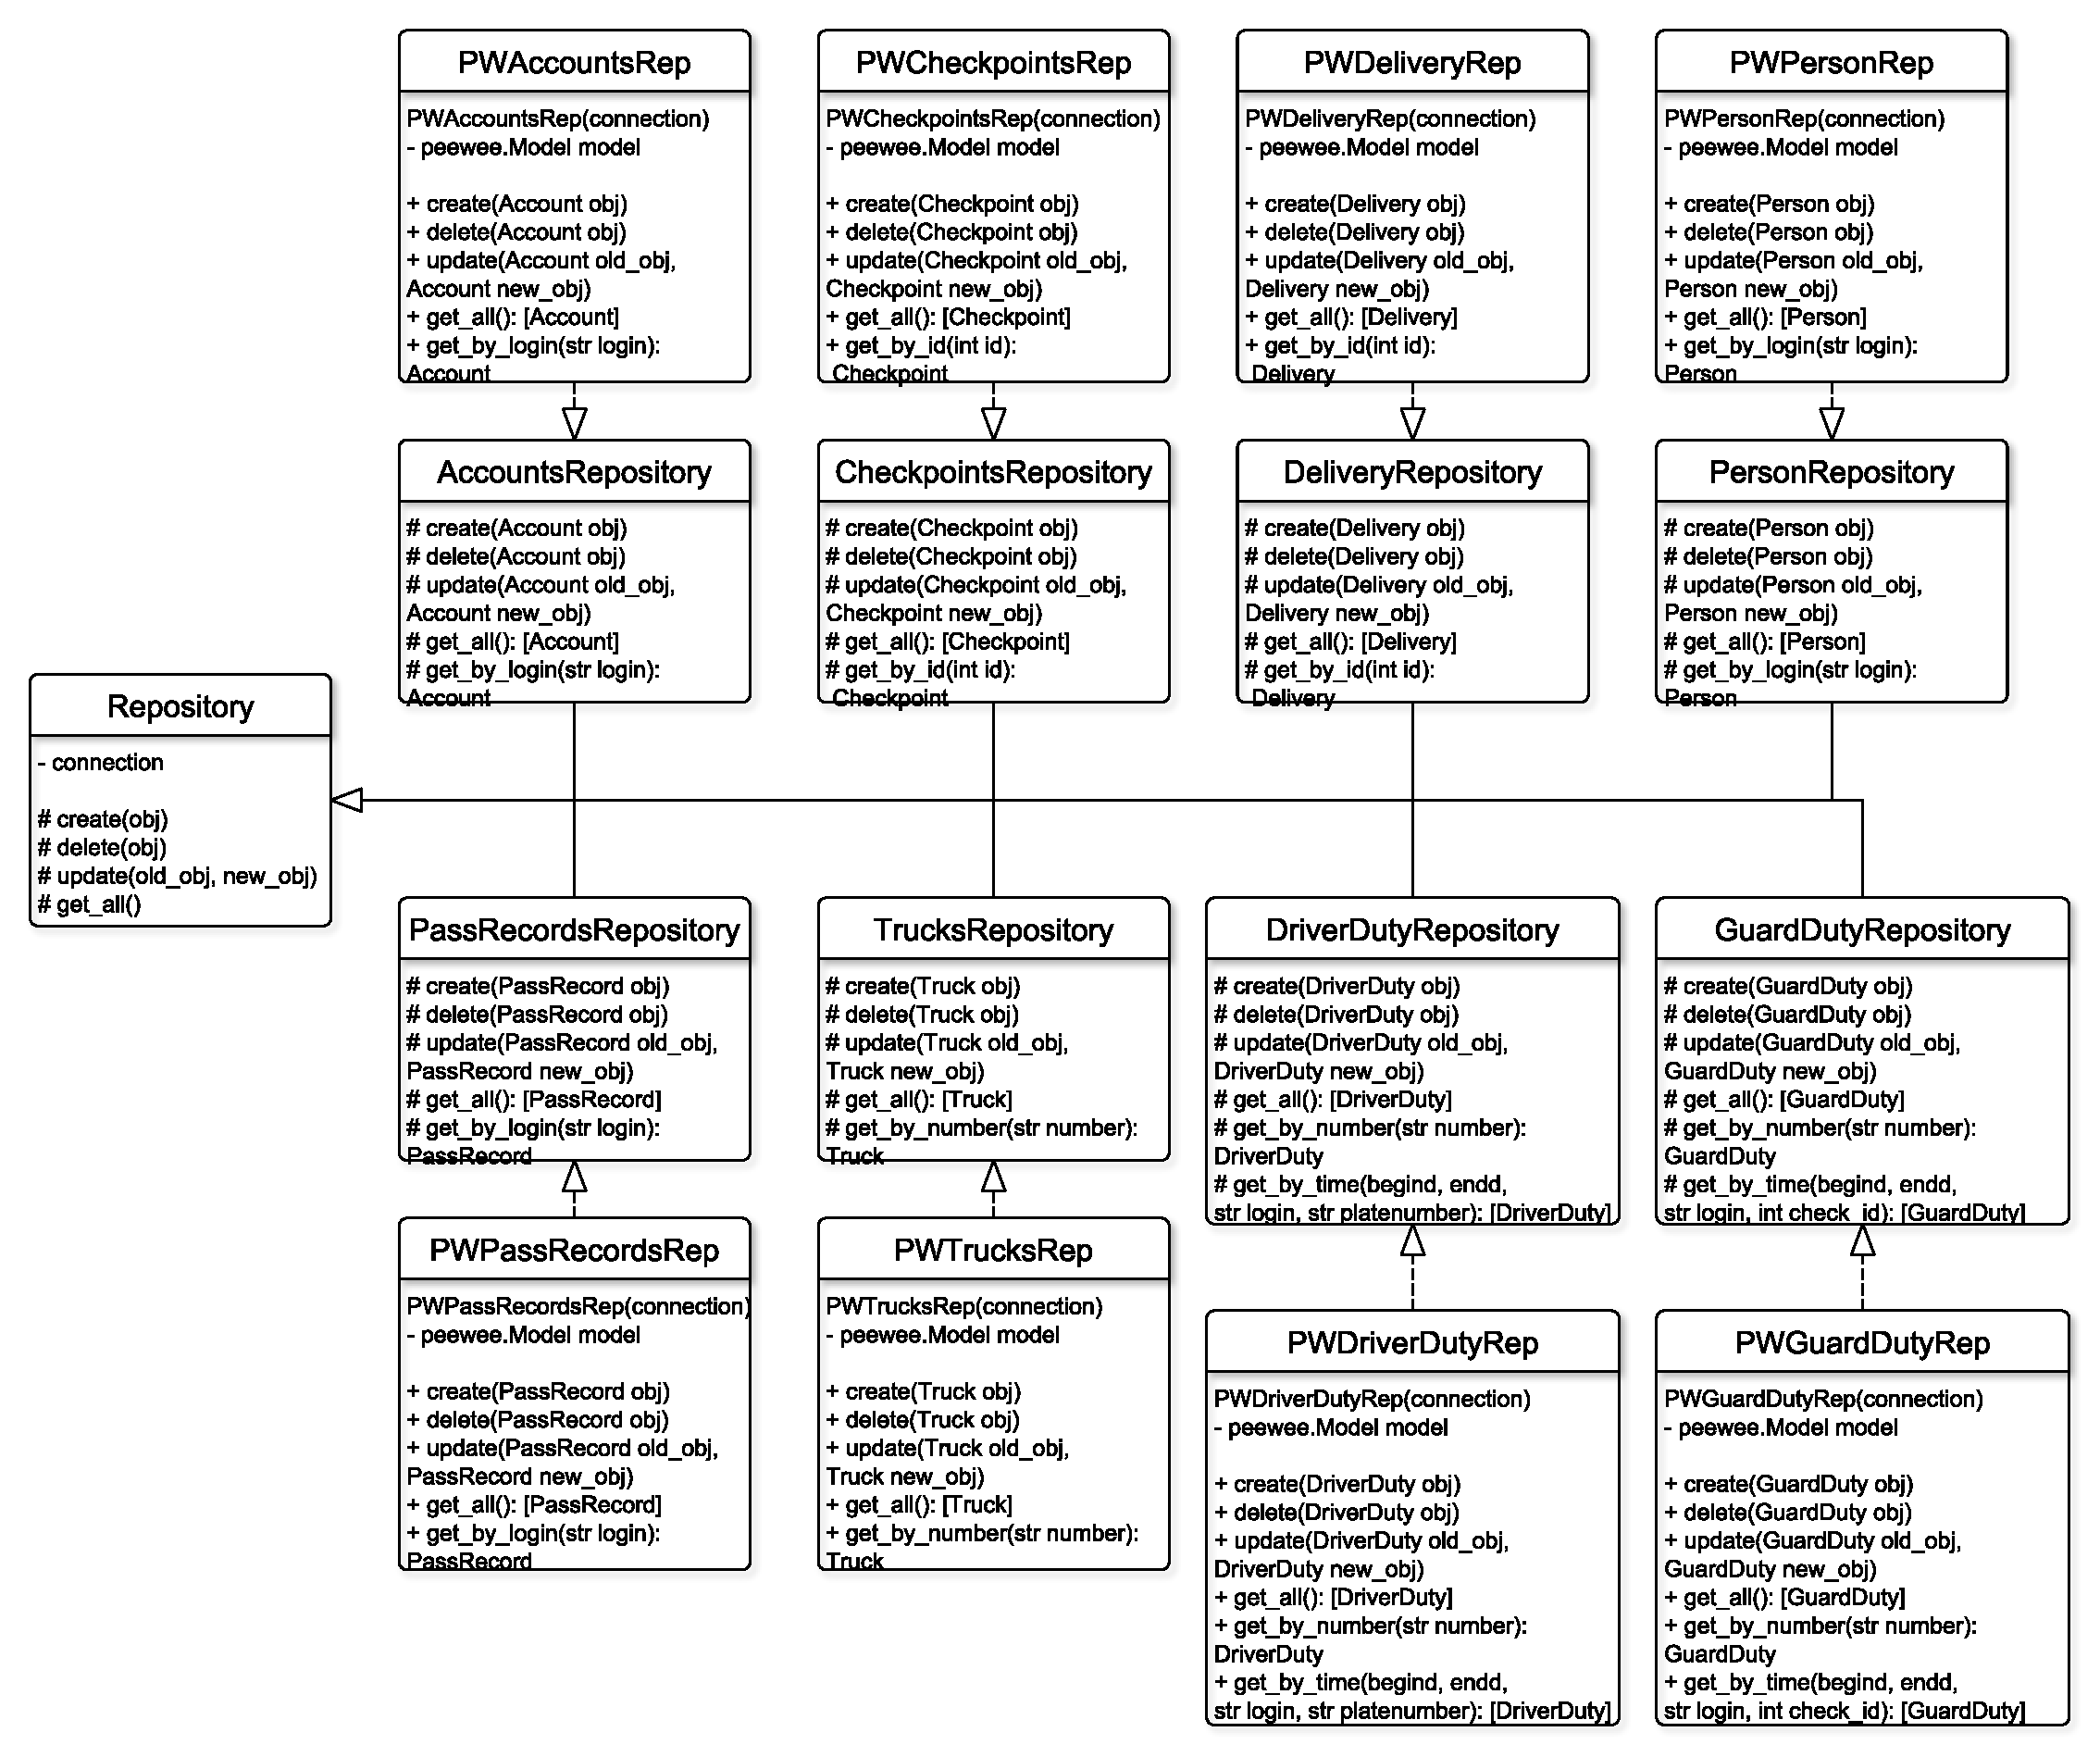
\includegraphics[height=14cm, width = 14cm]{uml/repsoitory.pdf}}
		{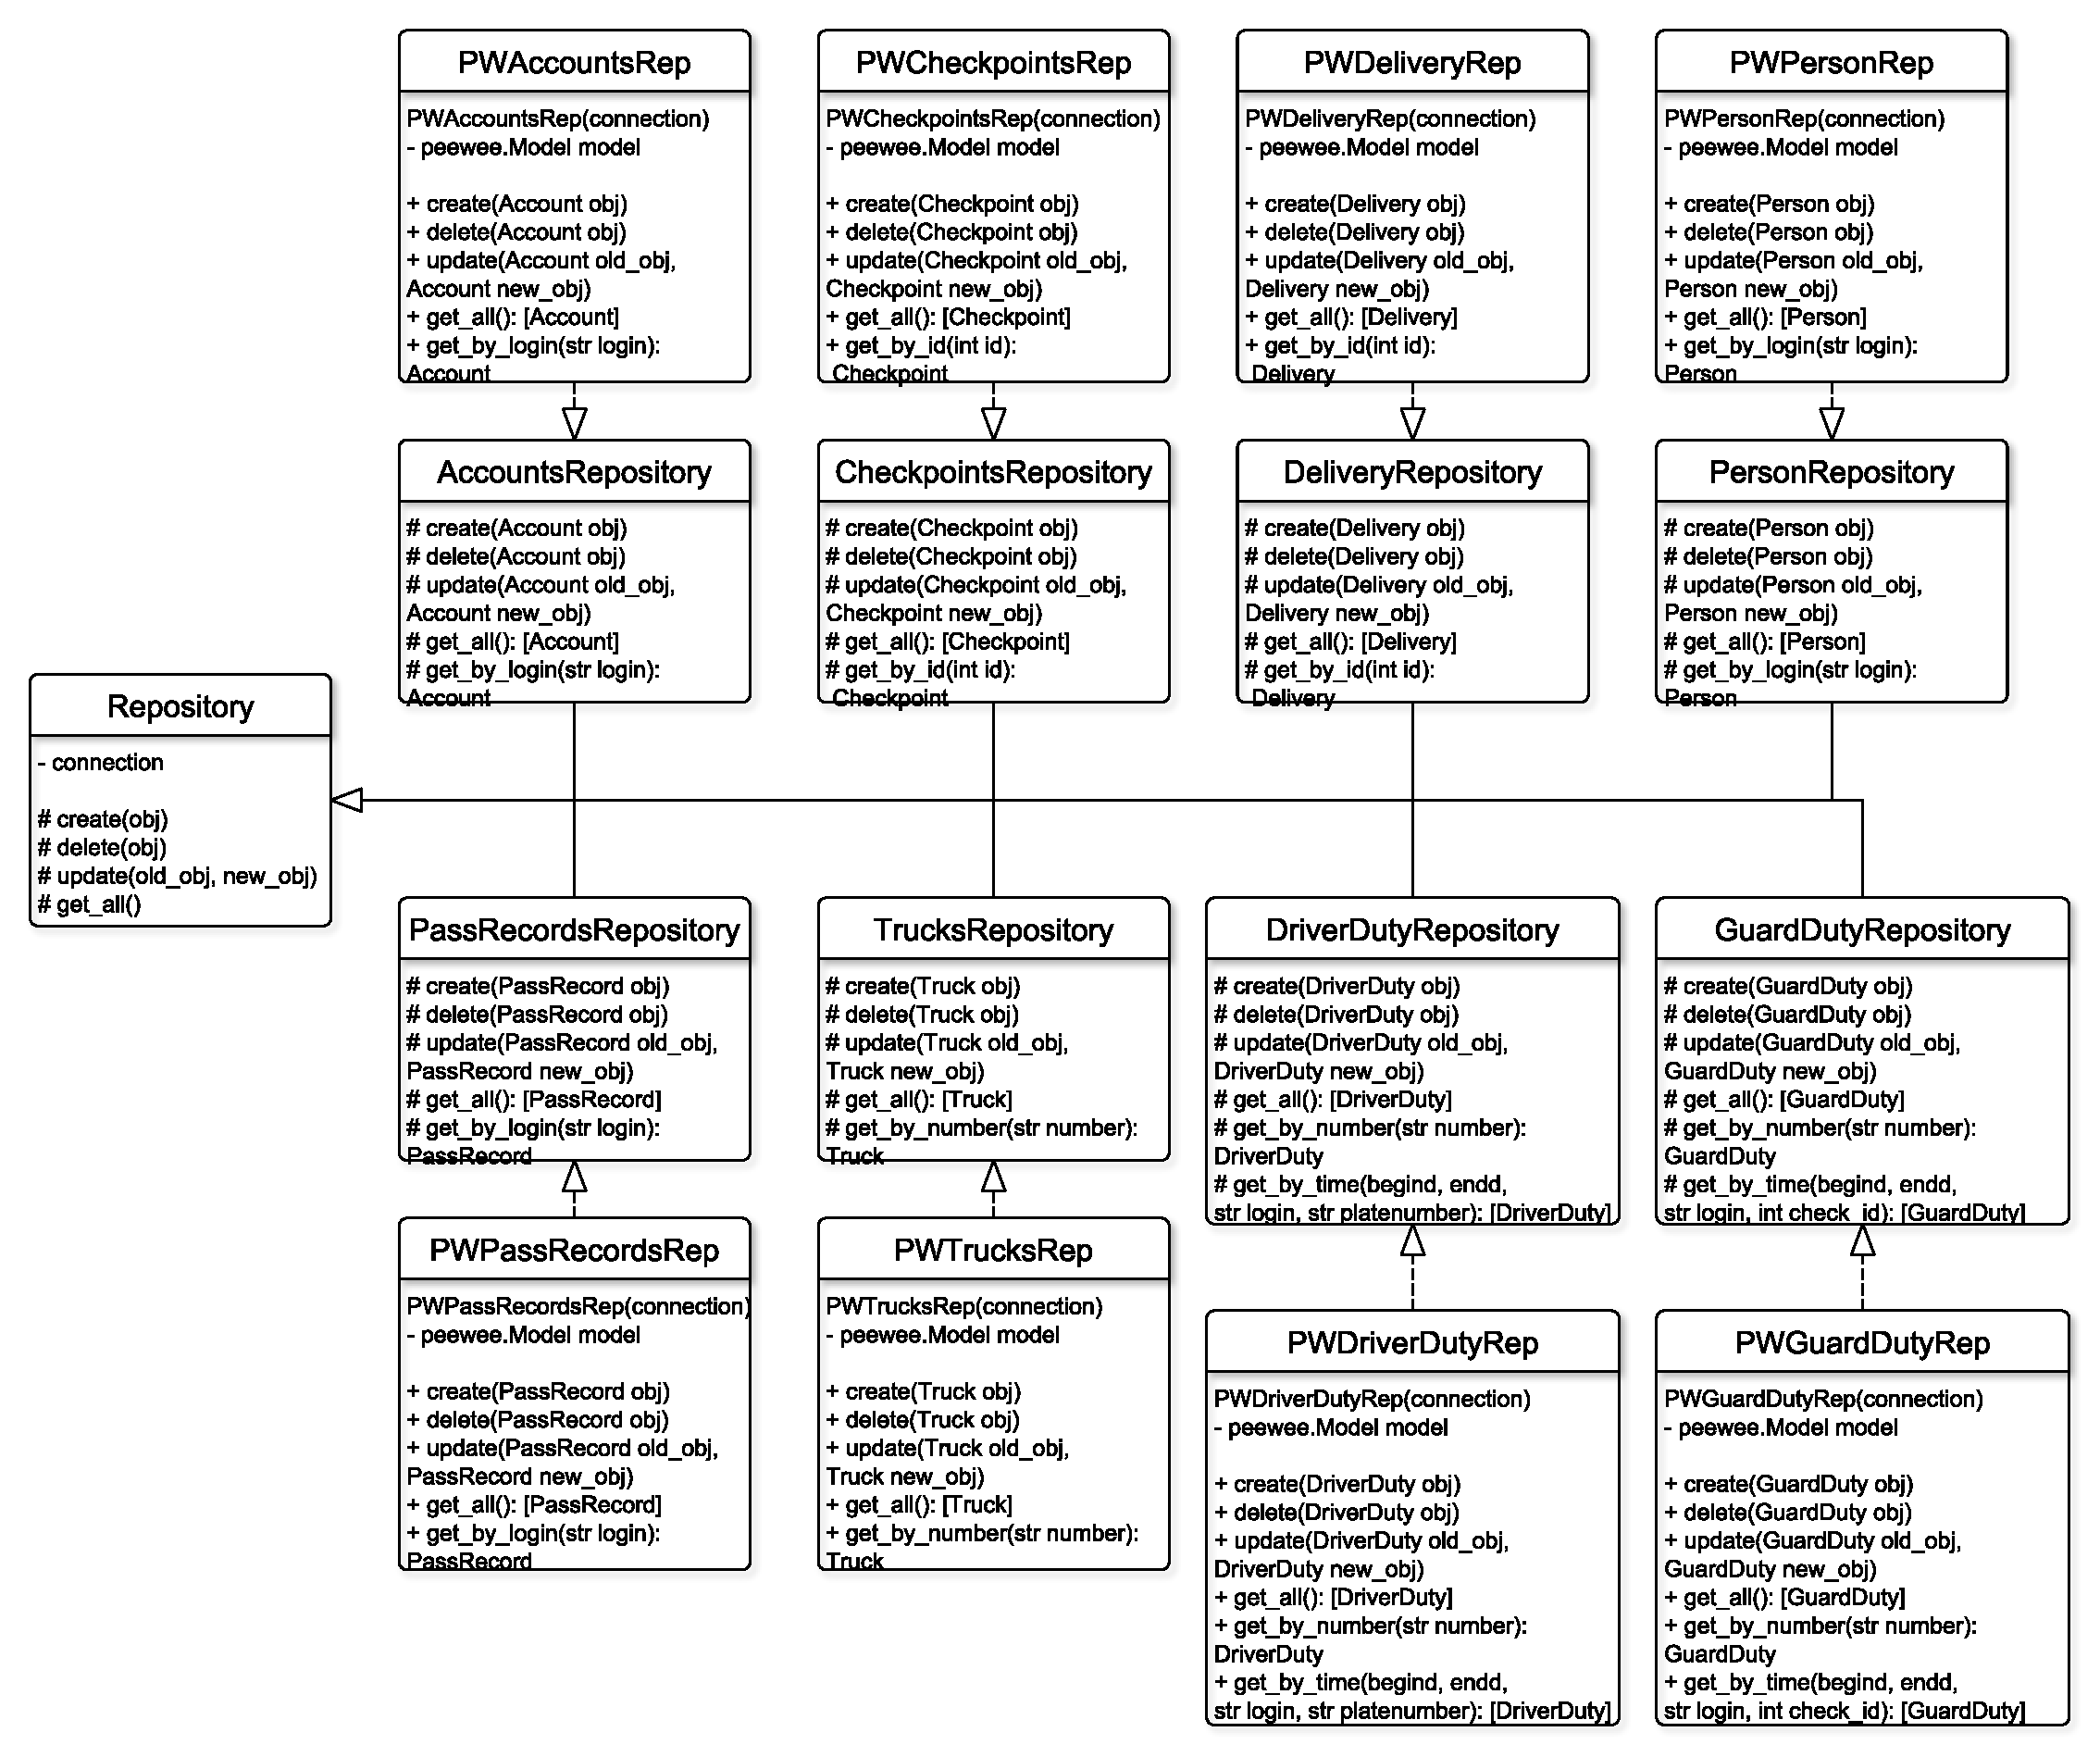
\includegraphics[scale=0.4, angle=0]{uml/repsoitory.pdf}}
		\caption{UML-диаграмма компонента доступа к данным}
		\label{rep_pic}
	\end{center}
\end{figure}

\newpage
\subsection{Компонент бизнес-логики}
В соответствии с подходом MVC был создан компонент бизнес-логики, выполняющий основную обработку данных, UML диаграмма которого представленна на рисунке \ref{model_pic}

\begin{figure}[h!] 
	\begin{center}
		%		{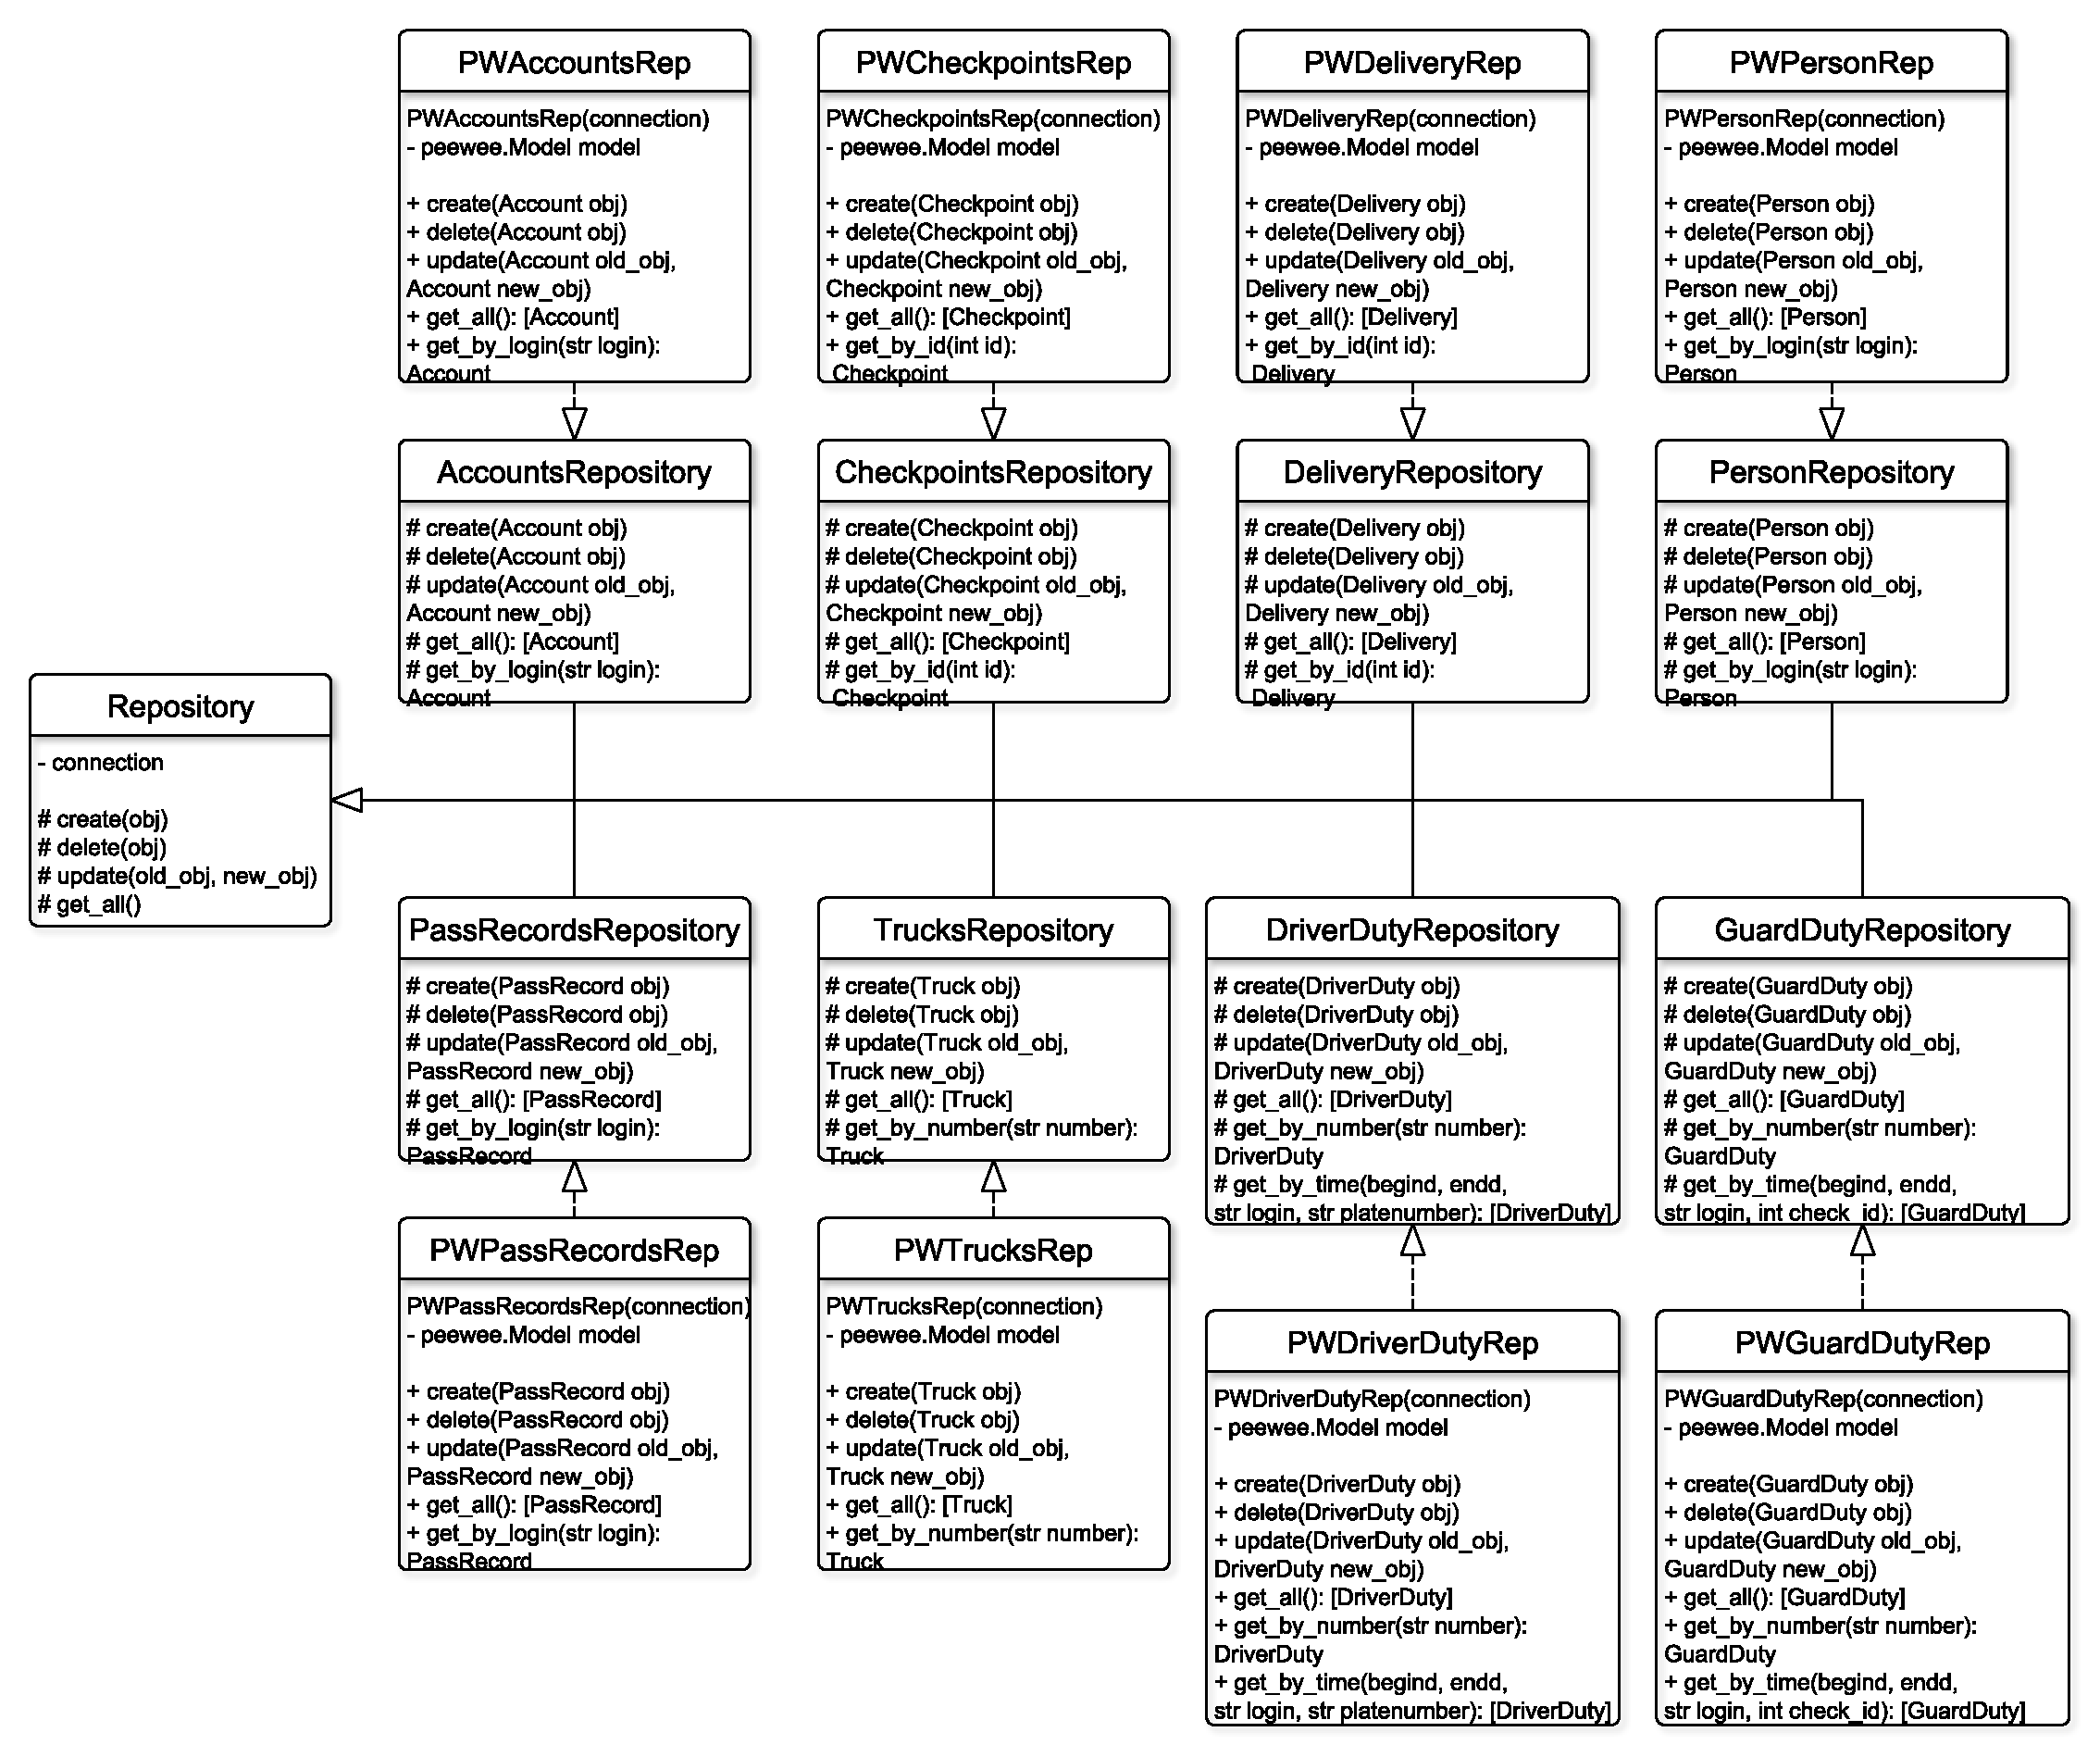
\includegraphics[height=14cm, width = 14cm]{uml/repsoitory.pdf}}
		{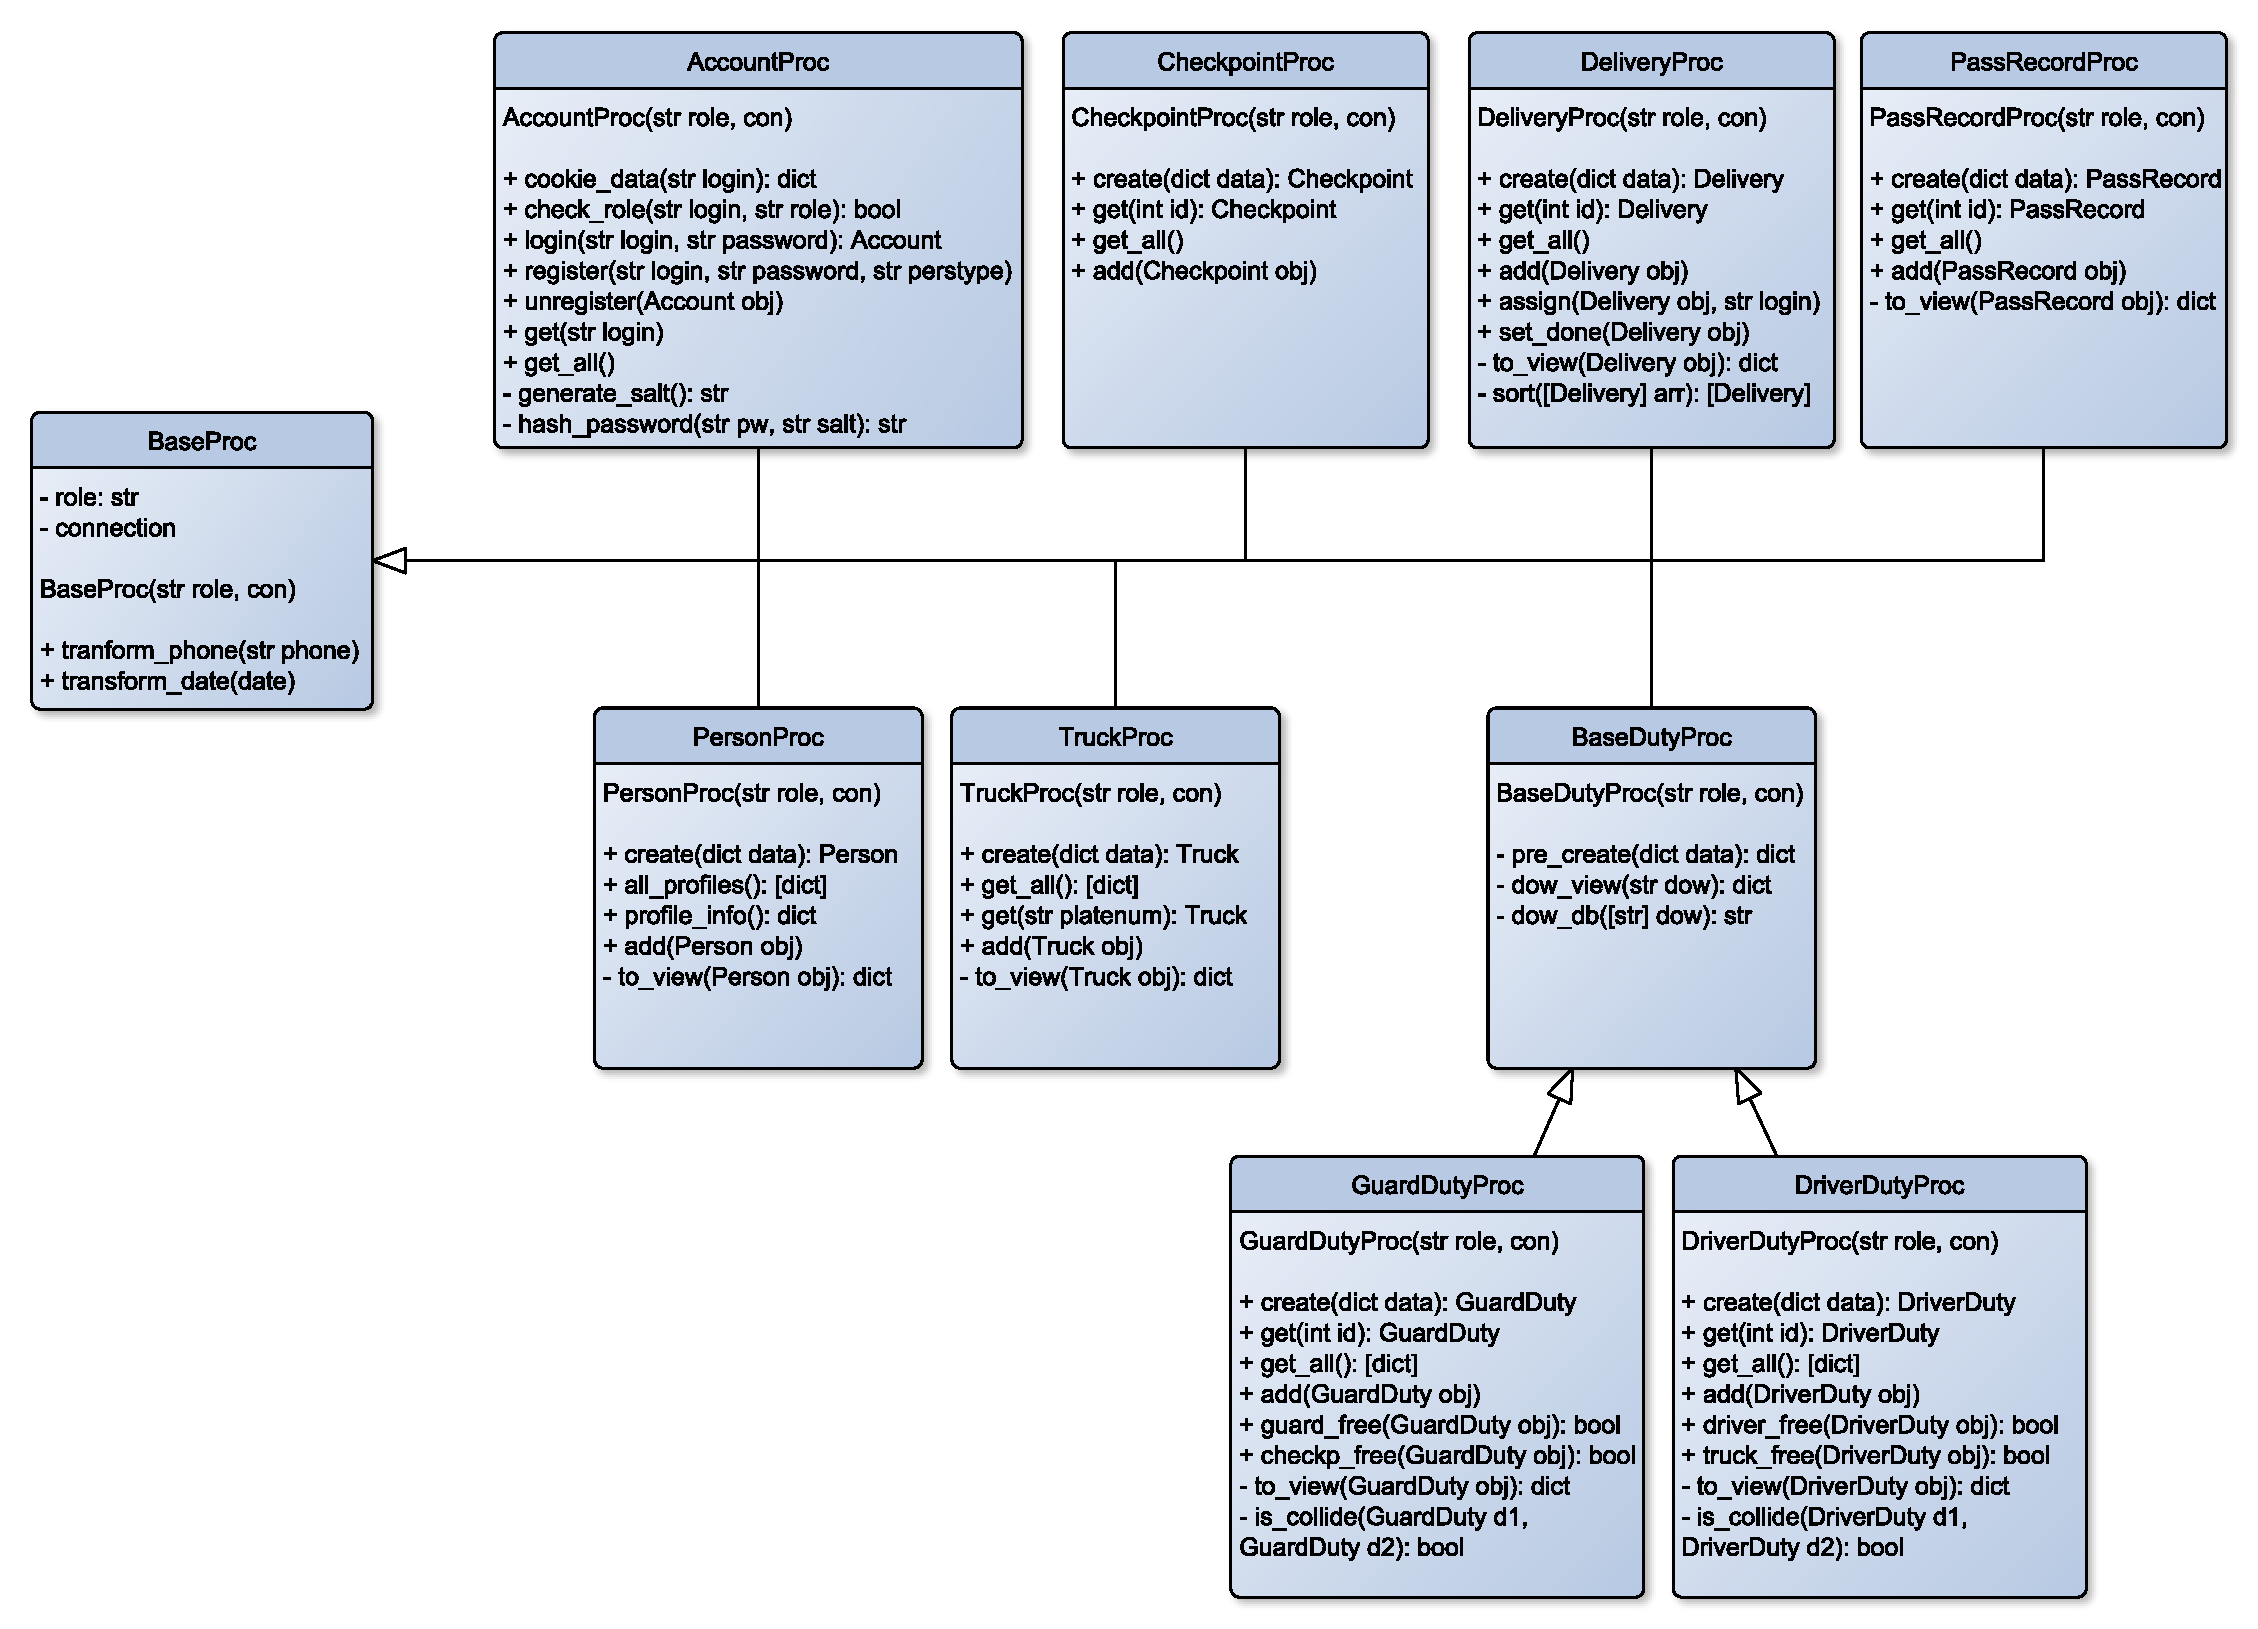
\includegraphics[scale=0.5, angle=0]{uml/business_models.pdf}}
		\caption{UML-диаграмма компонента бизнес-логики}
		\label{model_pic}
	\end{center}
\end{figure}

\newpage
\subsection{Компонент представления}
Также создан компонент представления, выполняющий отображение web-страниц в ответ на запросы пользователя, UML диаграмма которого представленна на рисунке \ref{view_pic}. Помимо этого был реализован технический компонент представления, отображающий информацию в символьном виде, для возможности тестирования компонента бизнес-логики.

\begin{figure}[h!] 
	\begin{center}
		%		{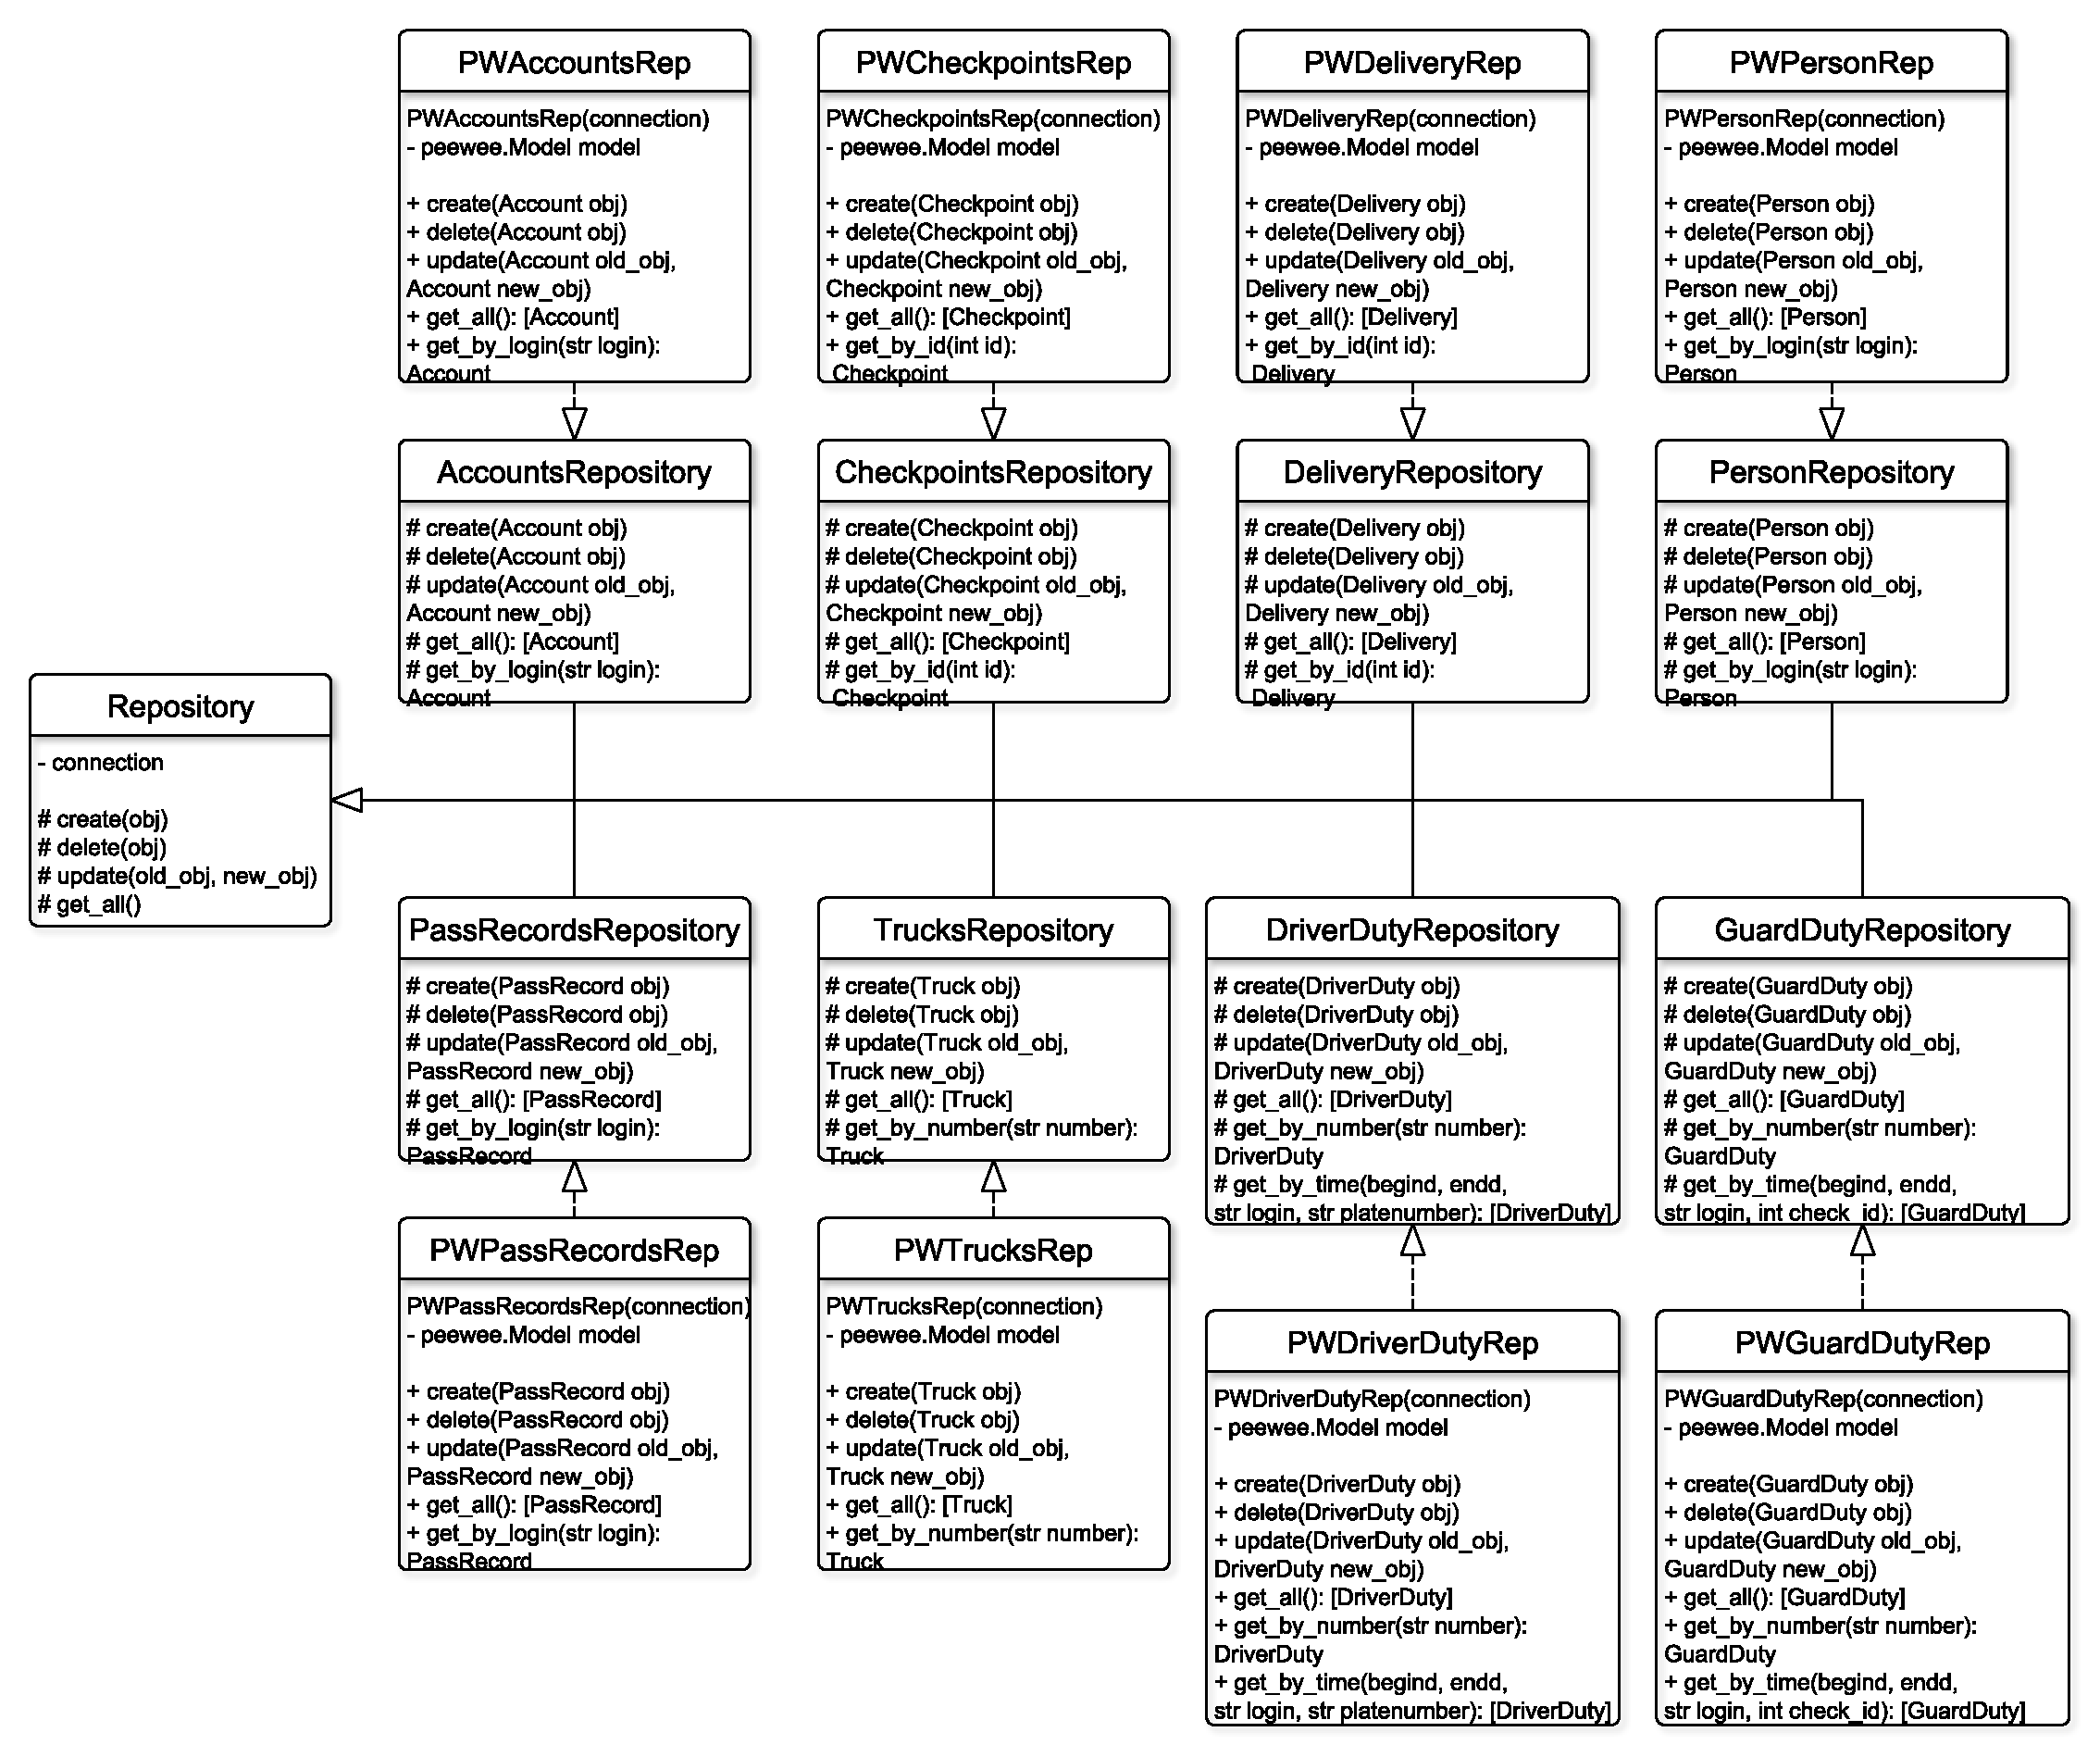
\includegraphics[height=14cm, width = 14cm]{uml/repsoitory.pdf}}
		{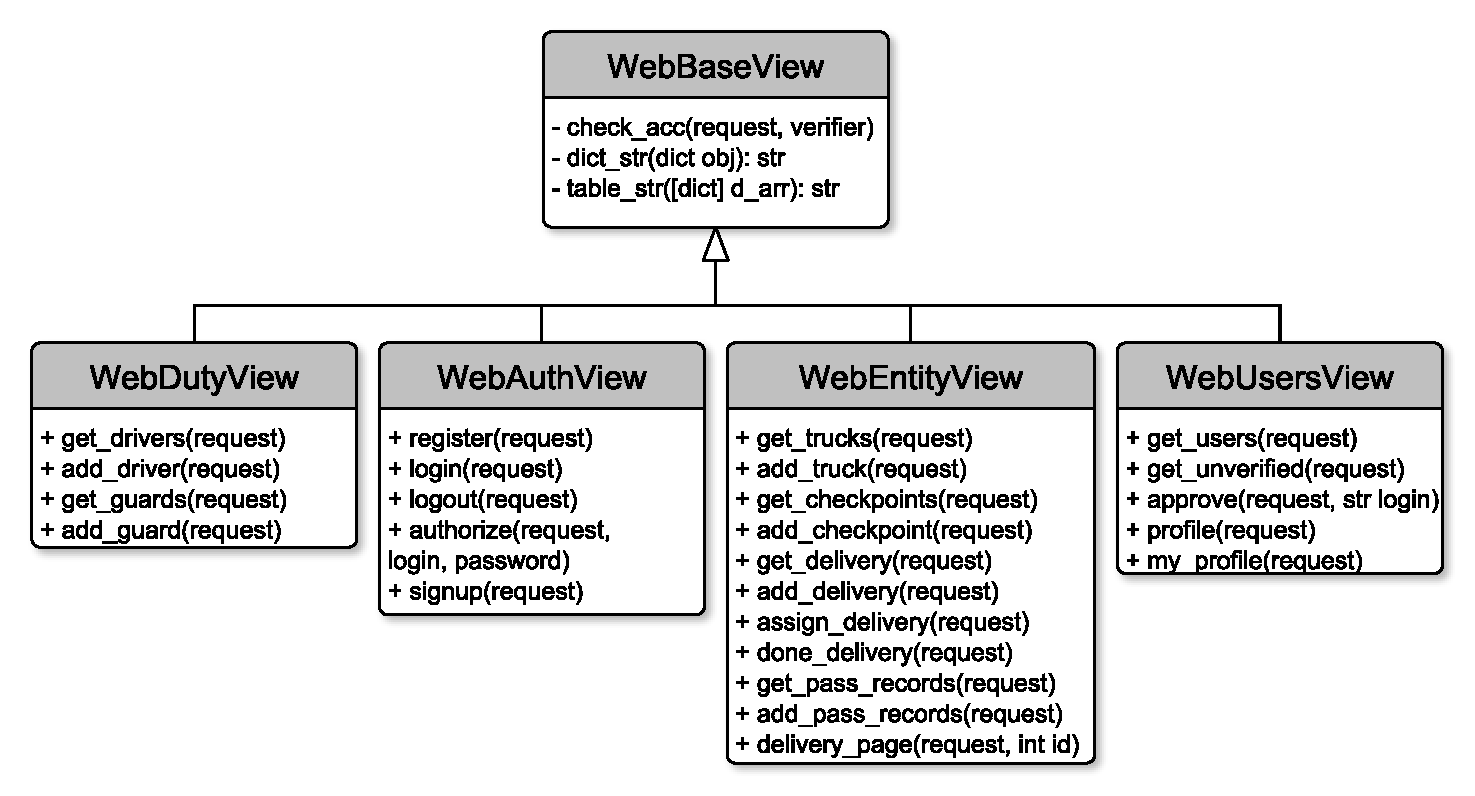
\includegraphics[scale=0.5, angle=0]{uml/webGUI.pdf}}
		\caption{UML-диаграмма компонента web-представления}
		\label{view_pic}
	\end{center}
\end{figure}

\newpage
\subsection{Диаграмма приложения}
Все перечисленные компоненты можно объединить в одну UML-диаграмму всего приложения на рисунке \ref{alluml_pic}

\begin{figure}[h!] 
	\begin{center}
		%		{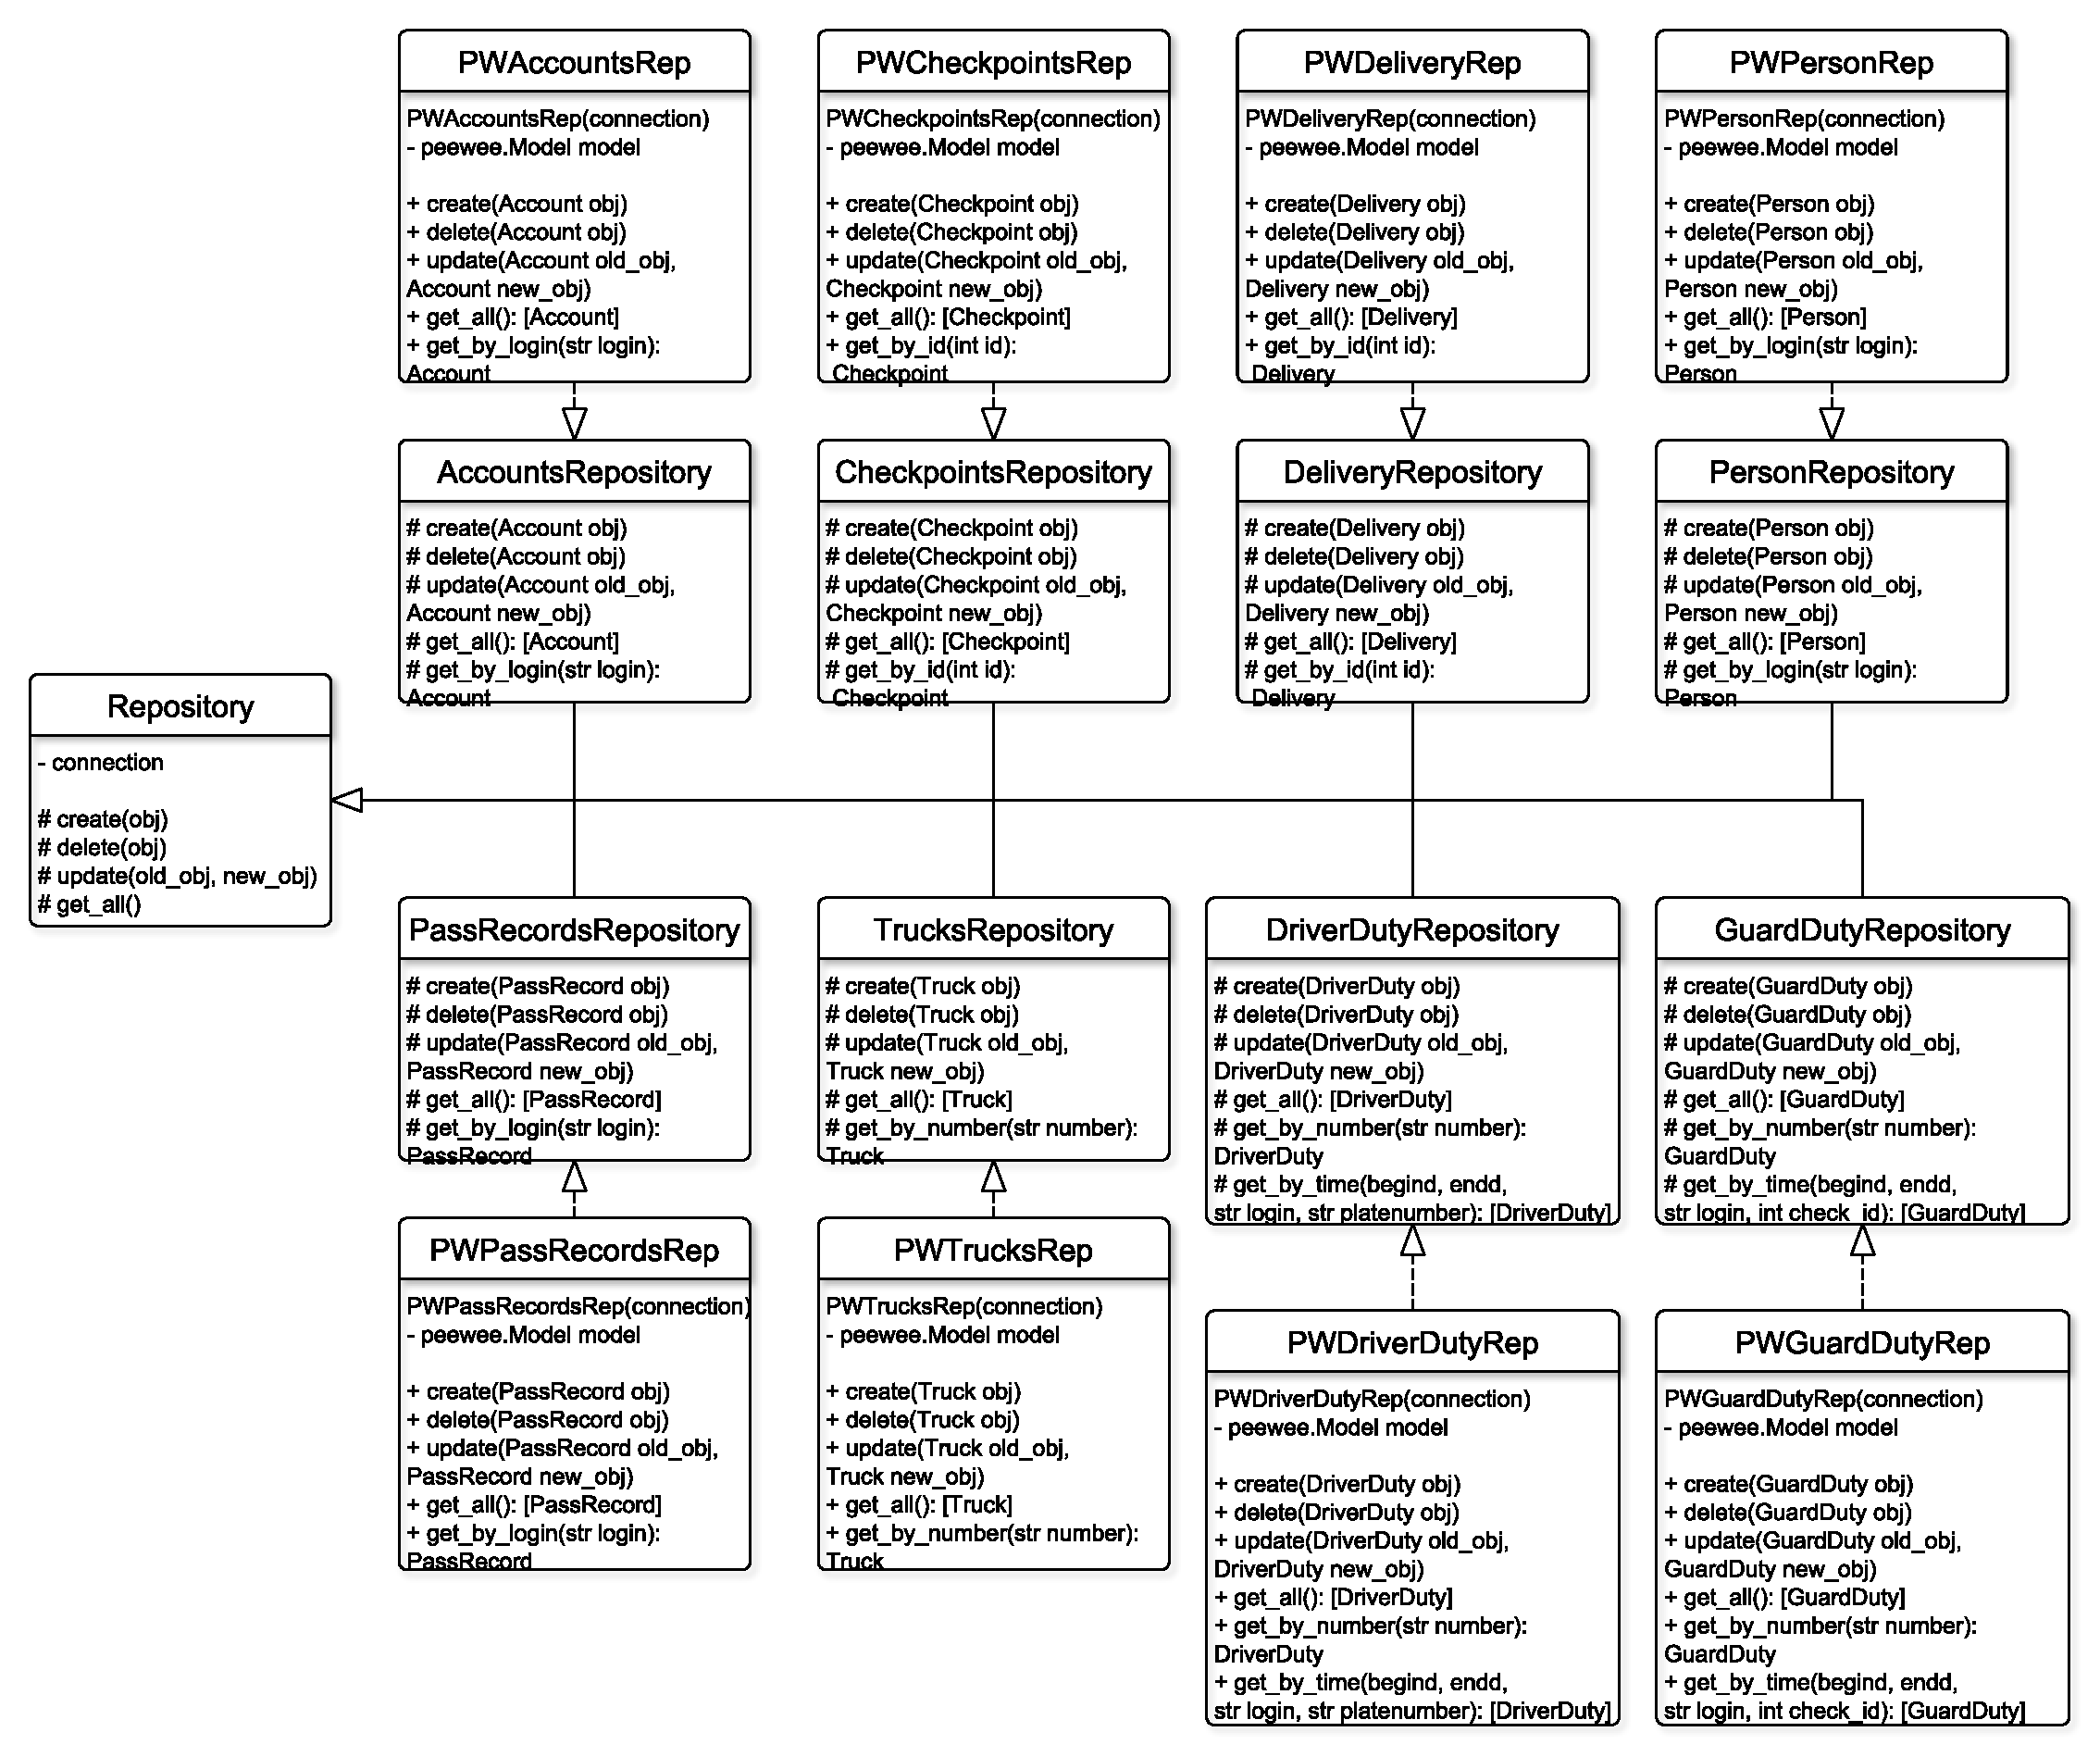
\includegraphics[height=14cm, width = 14cm]{uml/repsoitory.pdf}}
		{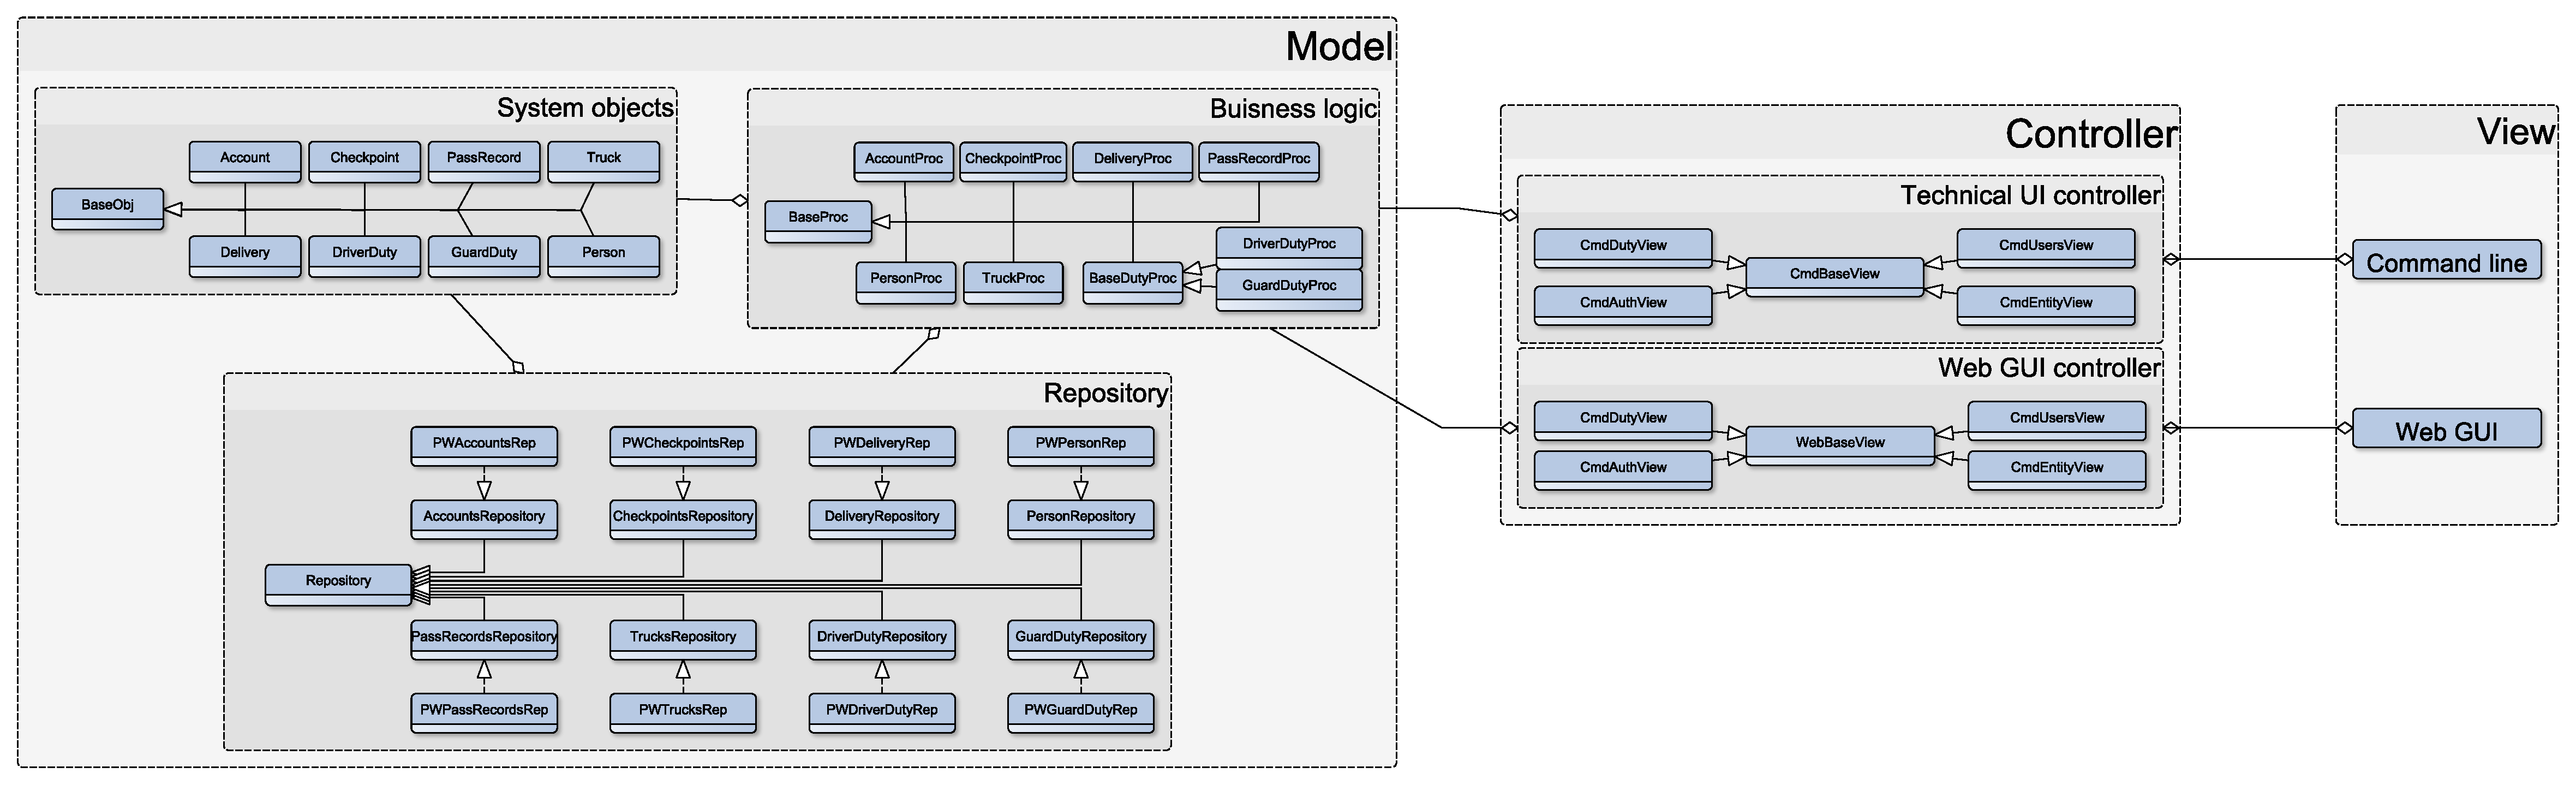
\includegraphics[scale=0.36, angle=-90]{uml/components.pdf}}
		\caption{UML-диаграмма компонента web-представления}
		\label{alluml_pic}
	\end{center}
\end{figure}


\section{Интерфейс приложения}
Для авторизованного пользователя в заголовке каждой страницы содержится панель навигации, предоставляющая возможность перейти на все страницы, функционально соответствующие его роли. Данная панель изображена на примере администратора на рисунке \ref{navbar_sc}. Некоторые пункты меню являются выпадающими, их можно открыть наведением мыши. Также в левом углу панели присутствует элемент информационного или ошибочного сообщения.

На рисунках \ref{navbar_sc}-\ref{trucks_sc} приведена демонстрация ключевых страниц для роли администратора. На рисунках \ref{pick_delivery_sc}, \ref{driver_profile_sc} и \ref{guard_duty_sc}, \ref{pass_guard_sc} приведены страницы, уникальные для ролей водителя и охранника соотвественно.

\begin{figure}[h!] 
	\begin{center}
		%		{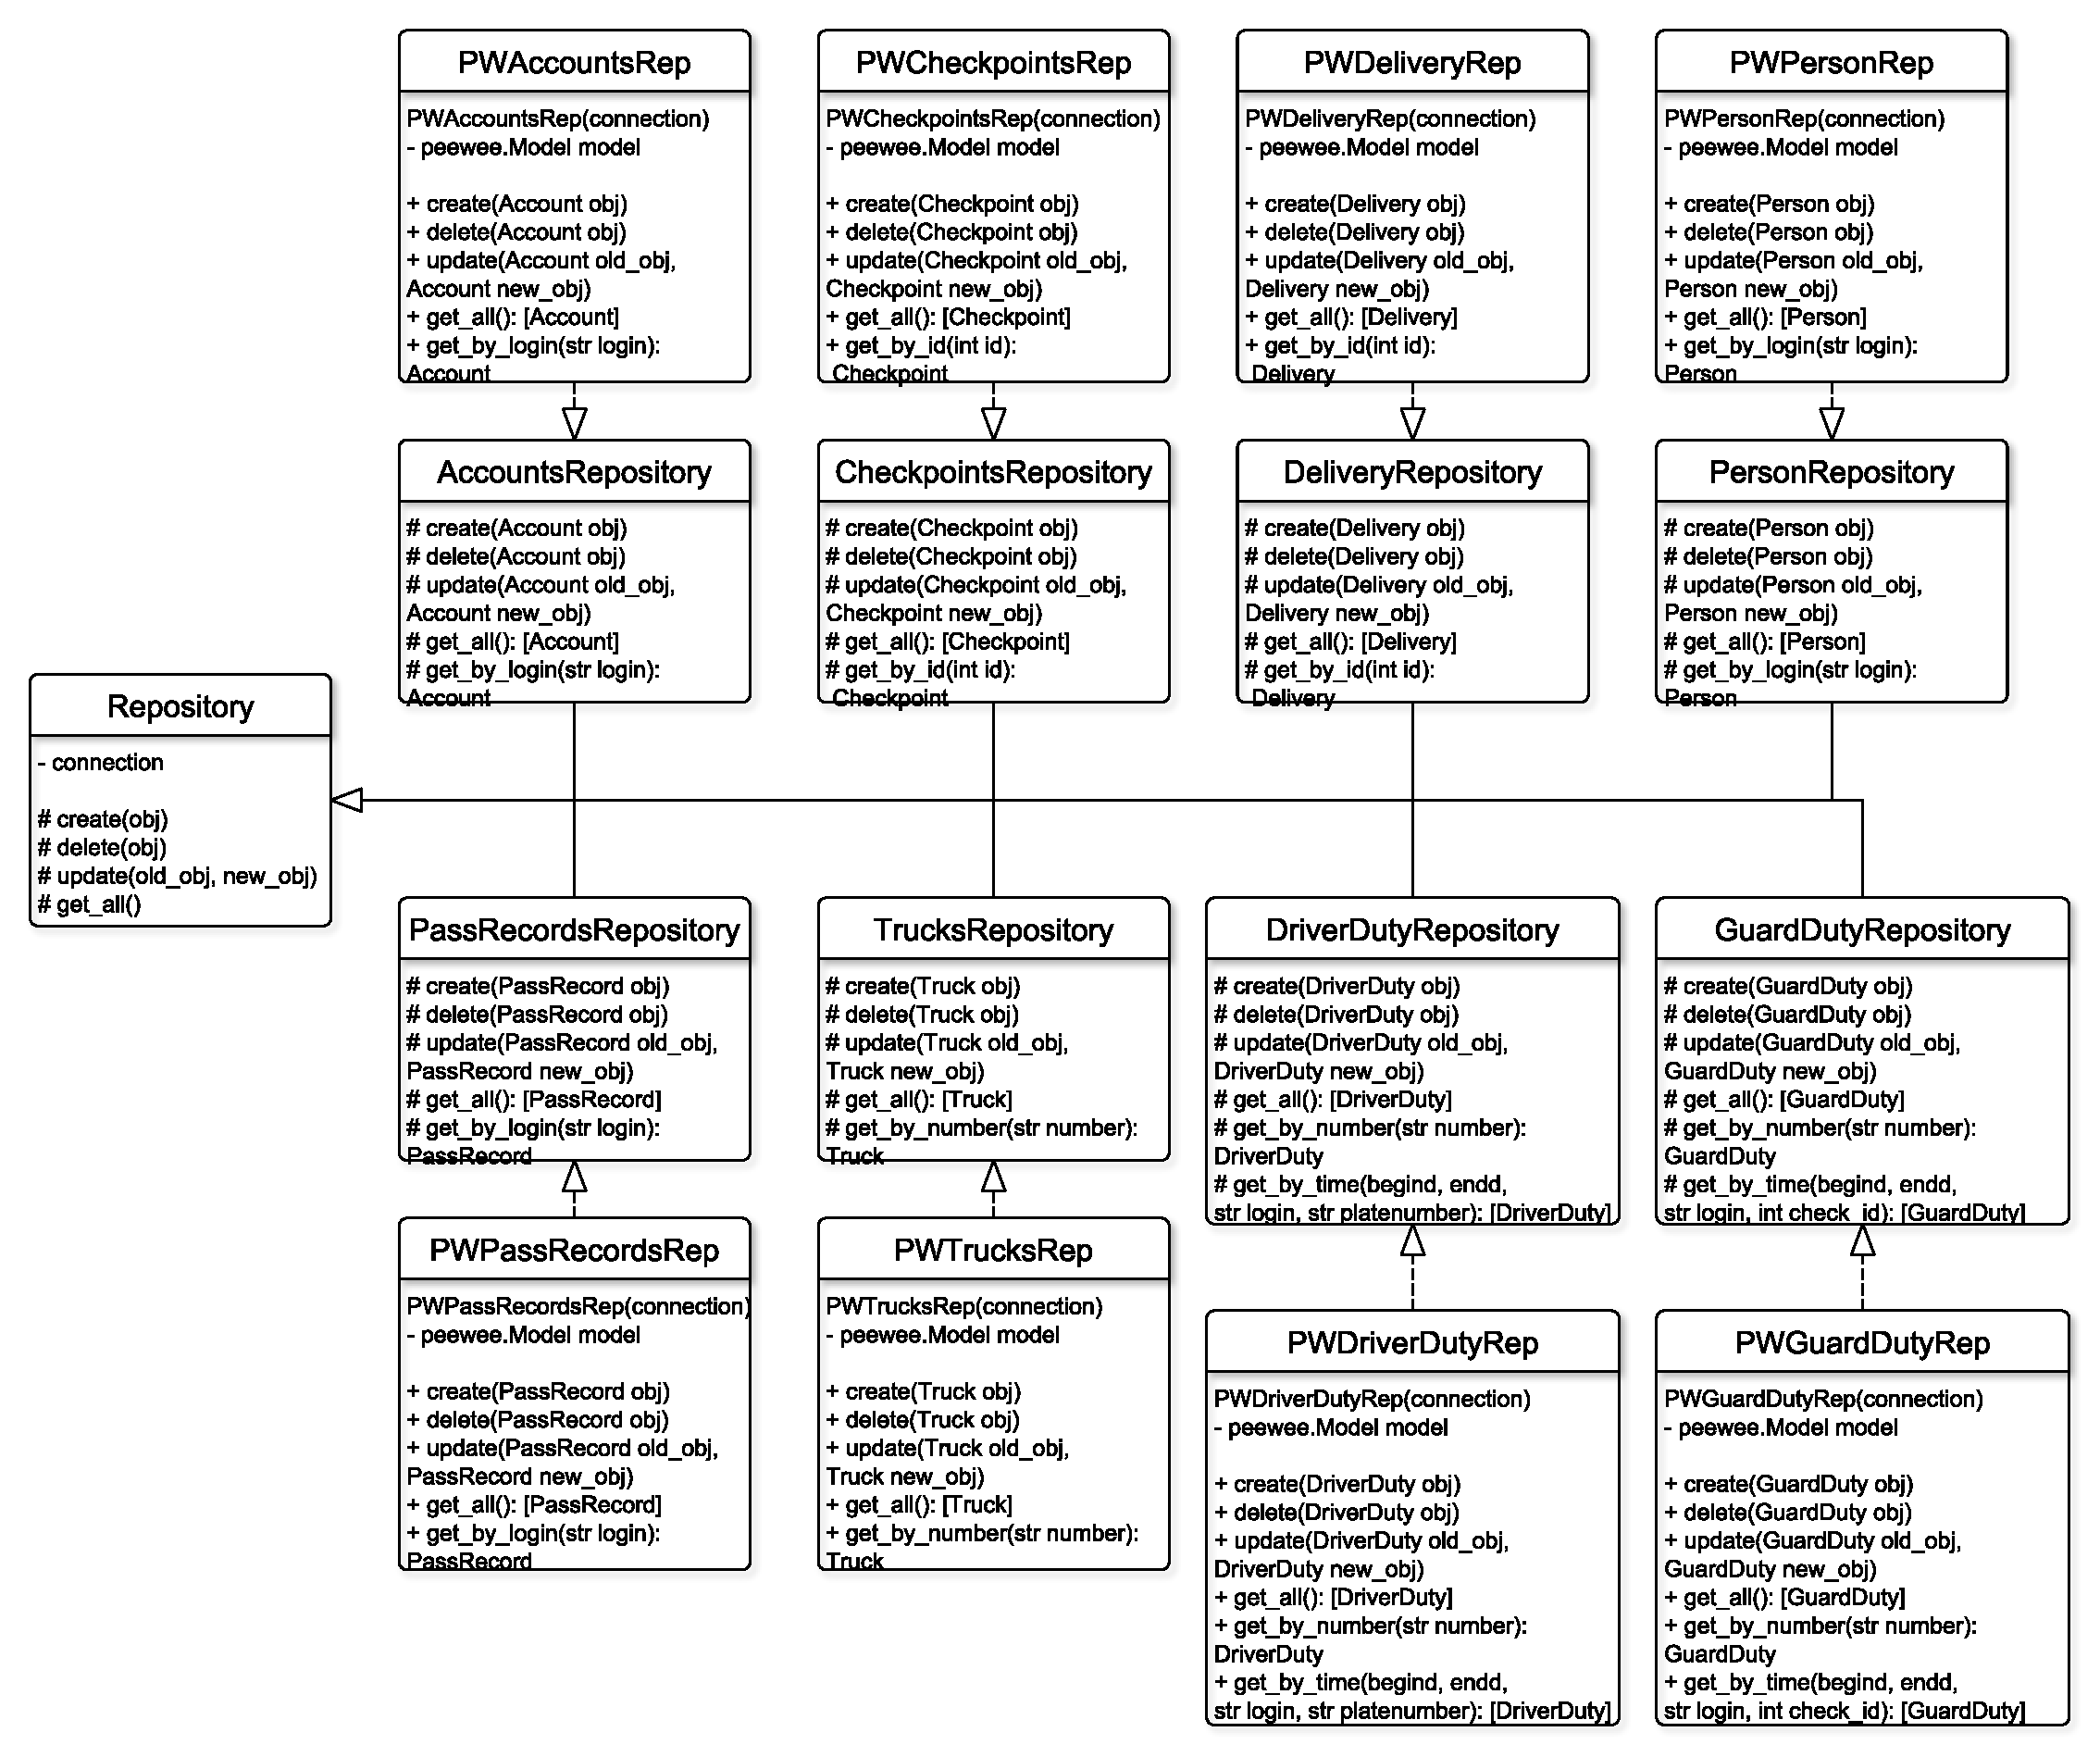
\includegraphics[height=14cm, width = 14cm]{uml/repsoitory.pdf}}
		{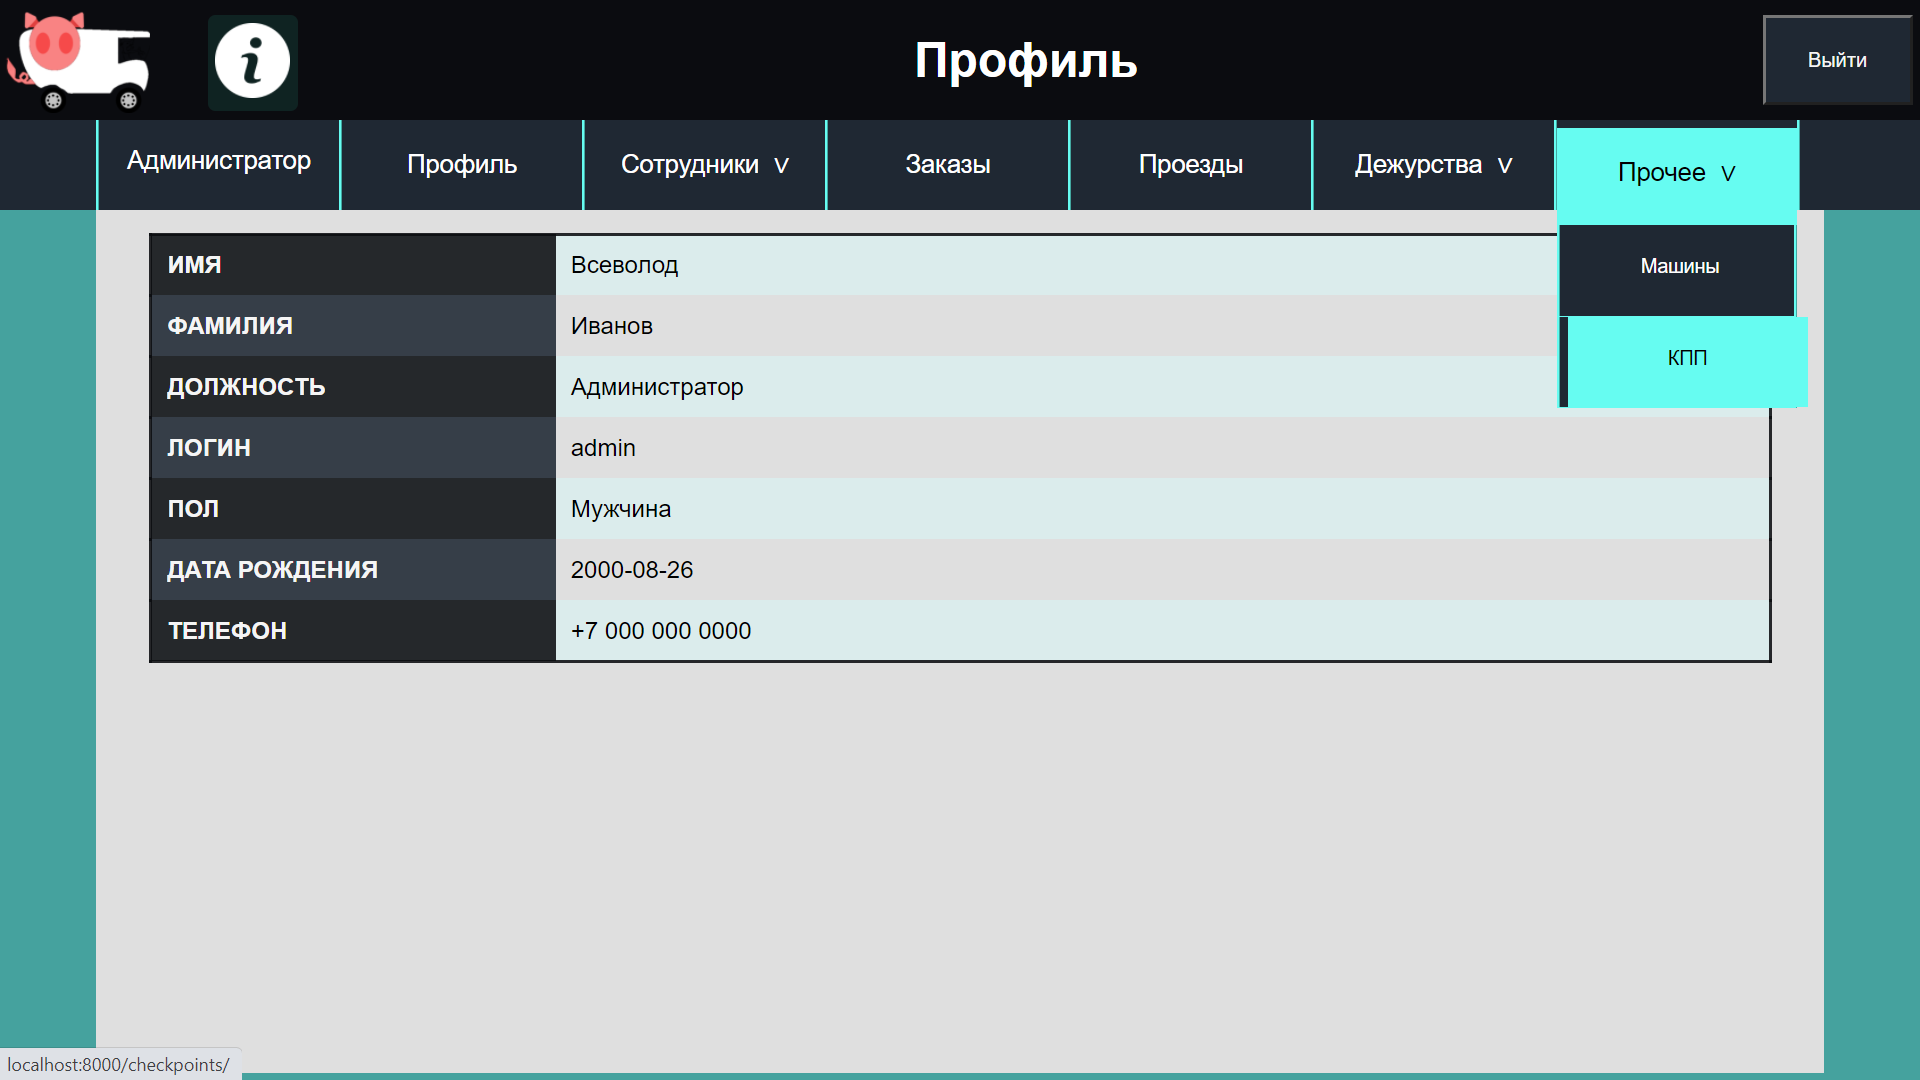
\includegraphics[scale=0.45, angle=0]{sc/admin_profile}}
		\caption{Страница профиля администратора}
		\label{navbar_sc}
	\end{center}
\end{figure}

\begin{figure}[h!] 
	\begin{center}
		%		{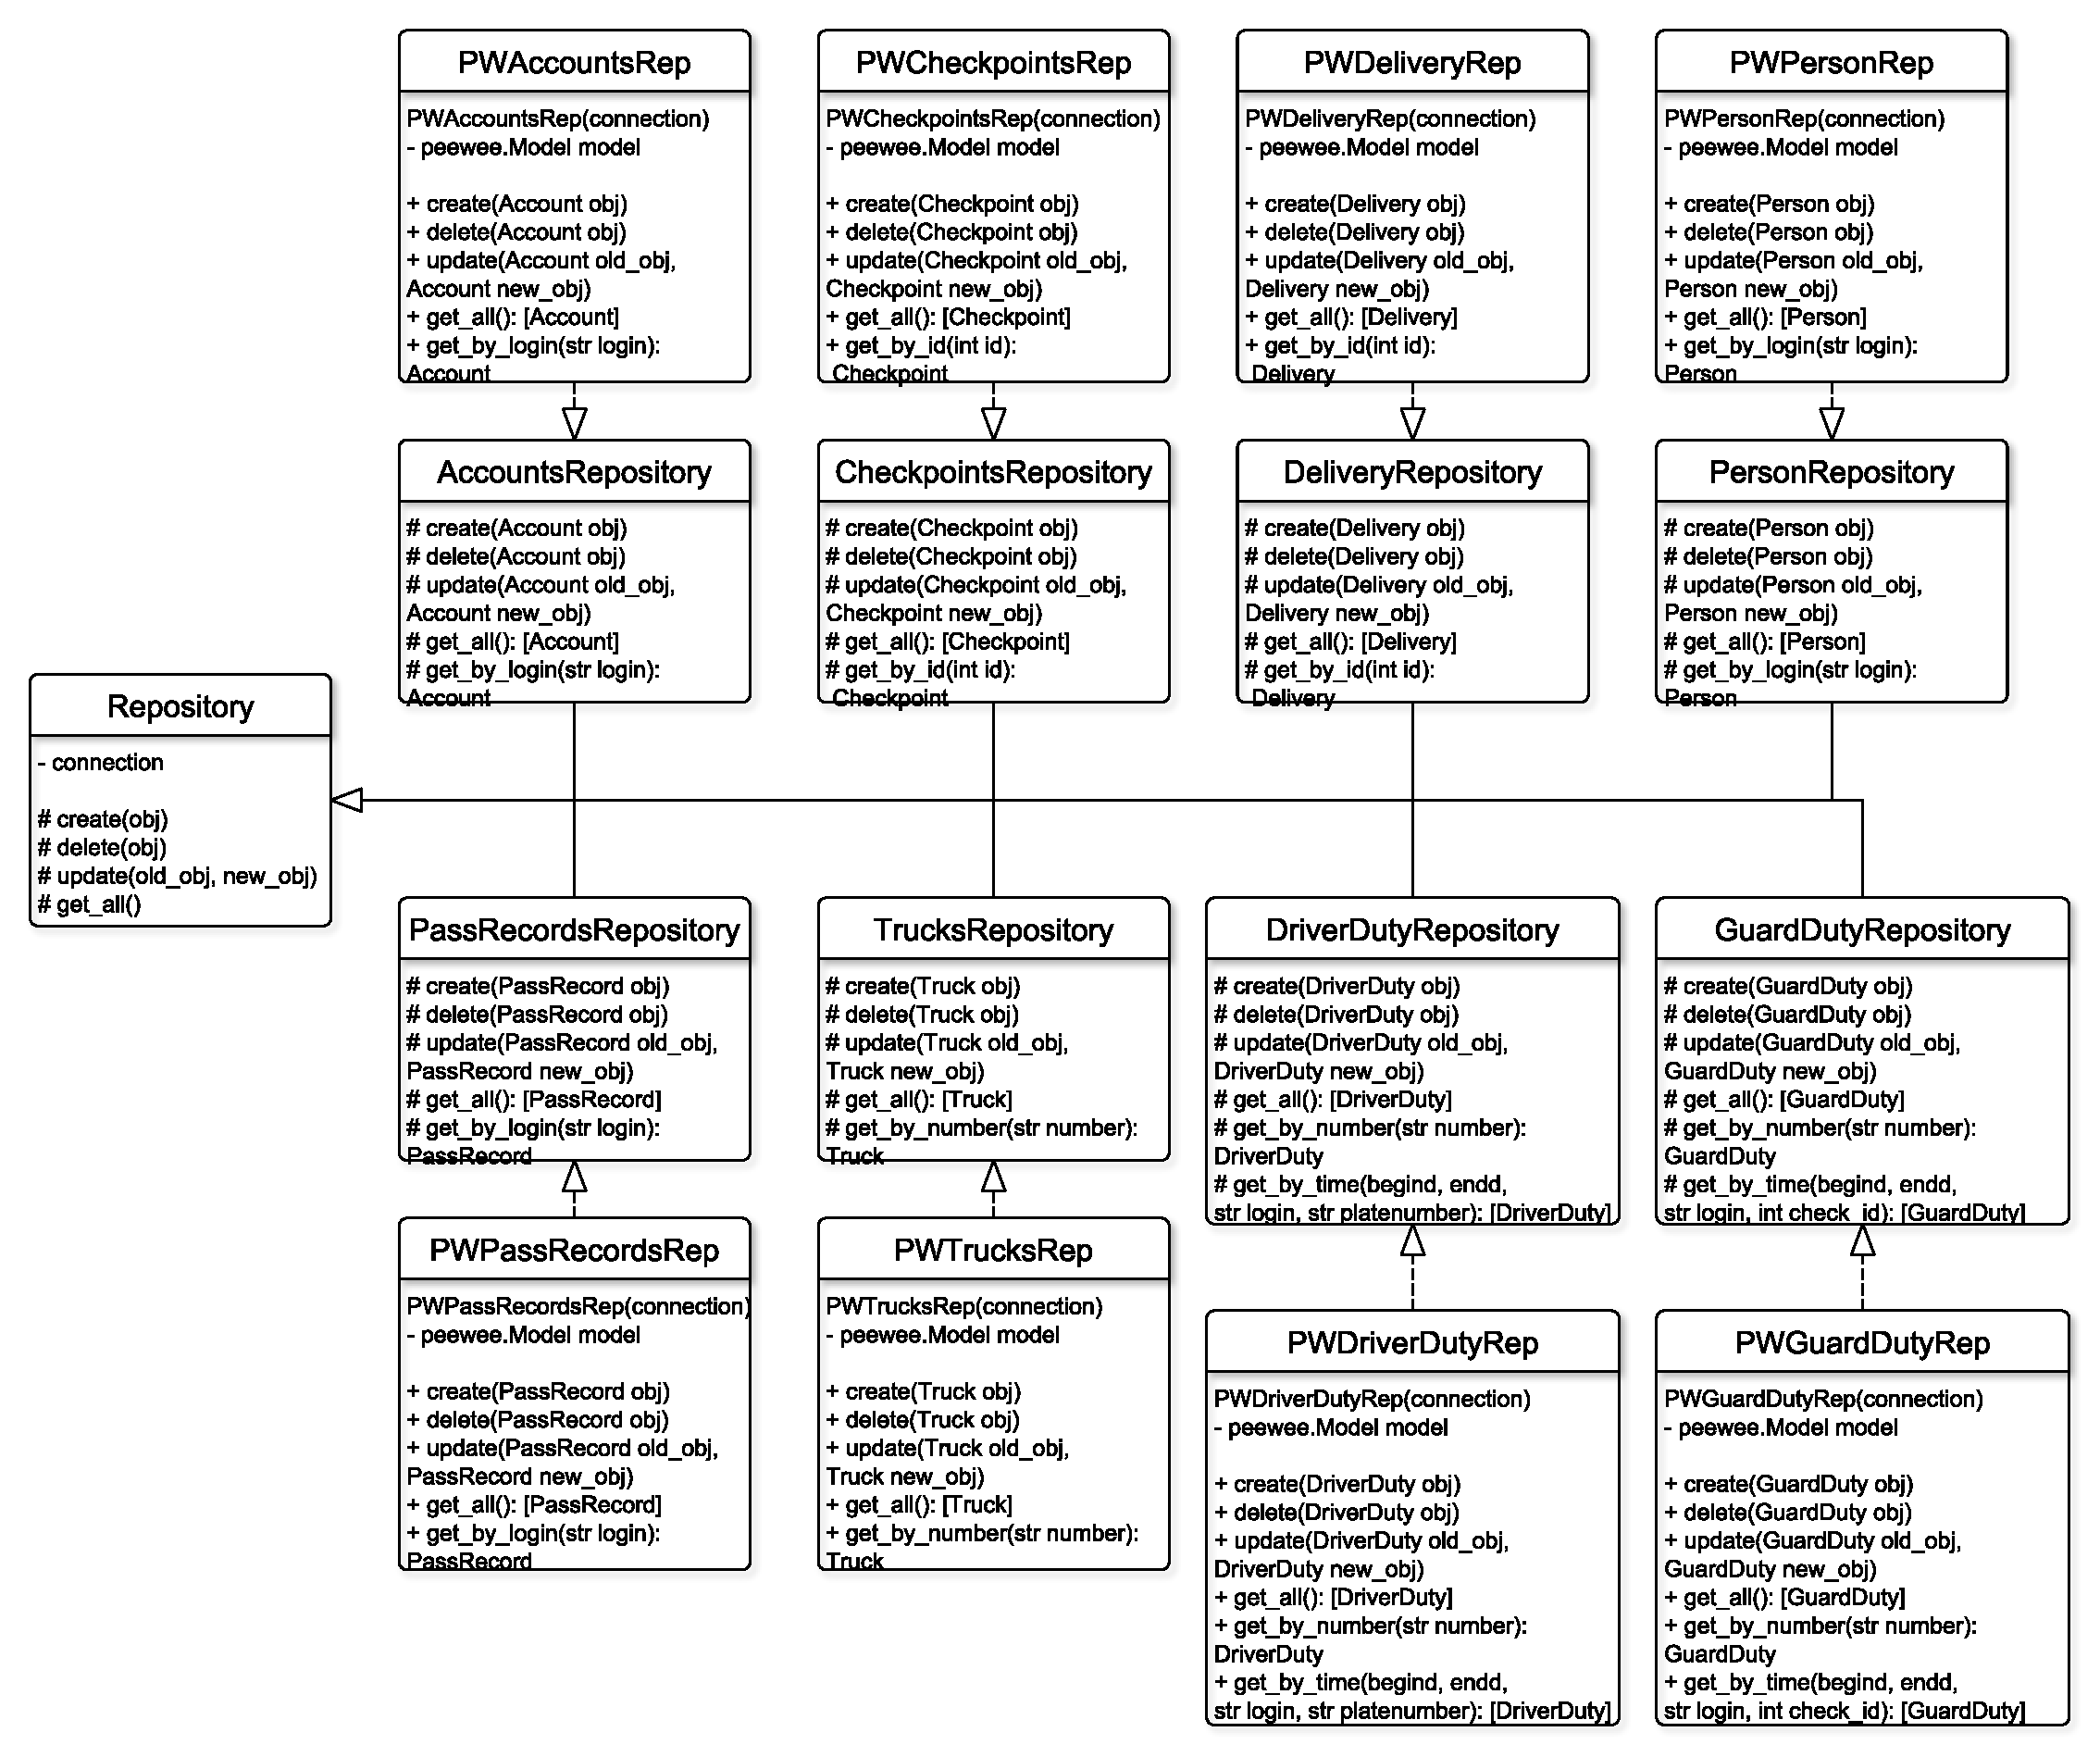
\includegraphics[height=14cm, width = 14cm]{uml/repsoitory.pdf}}
		{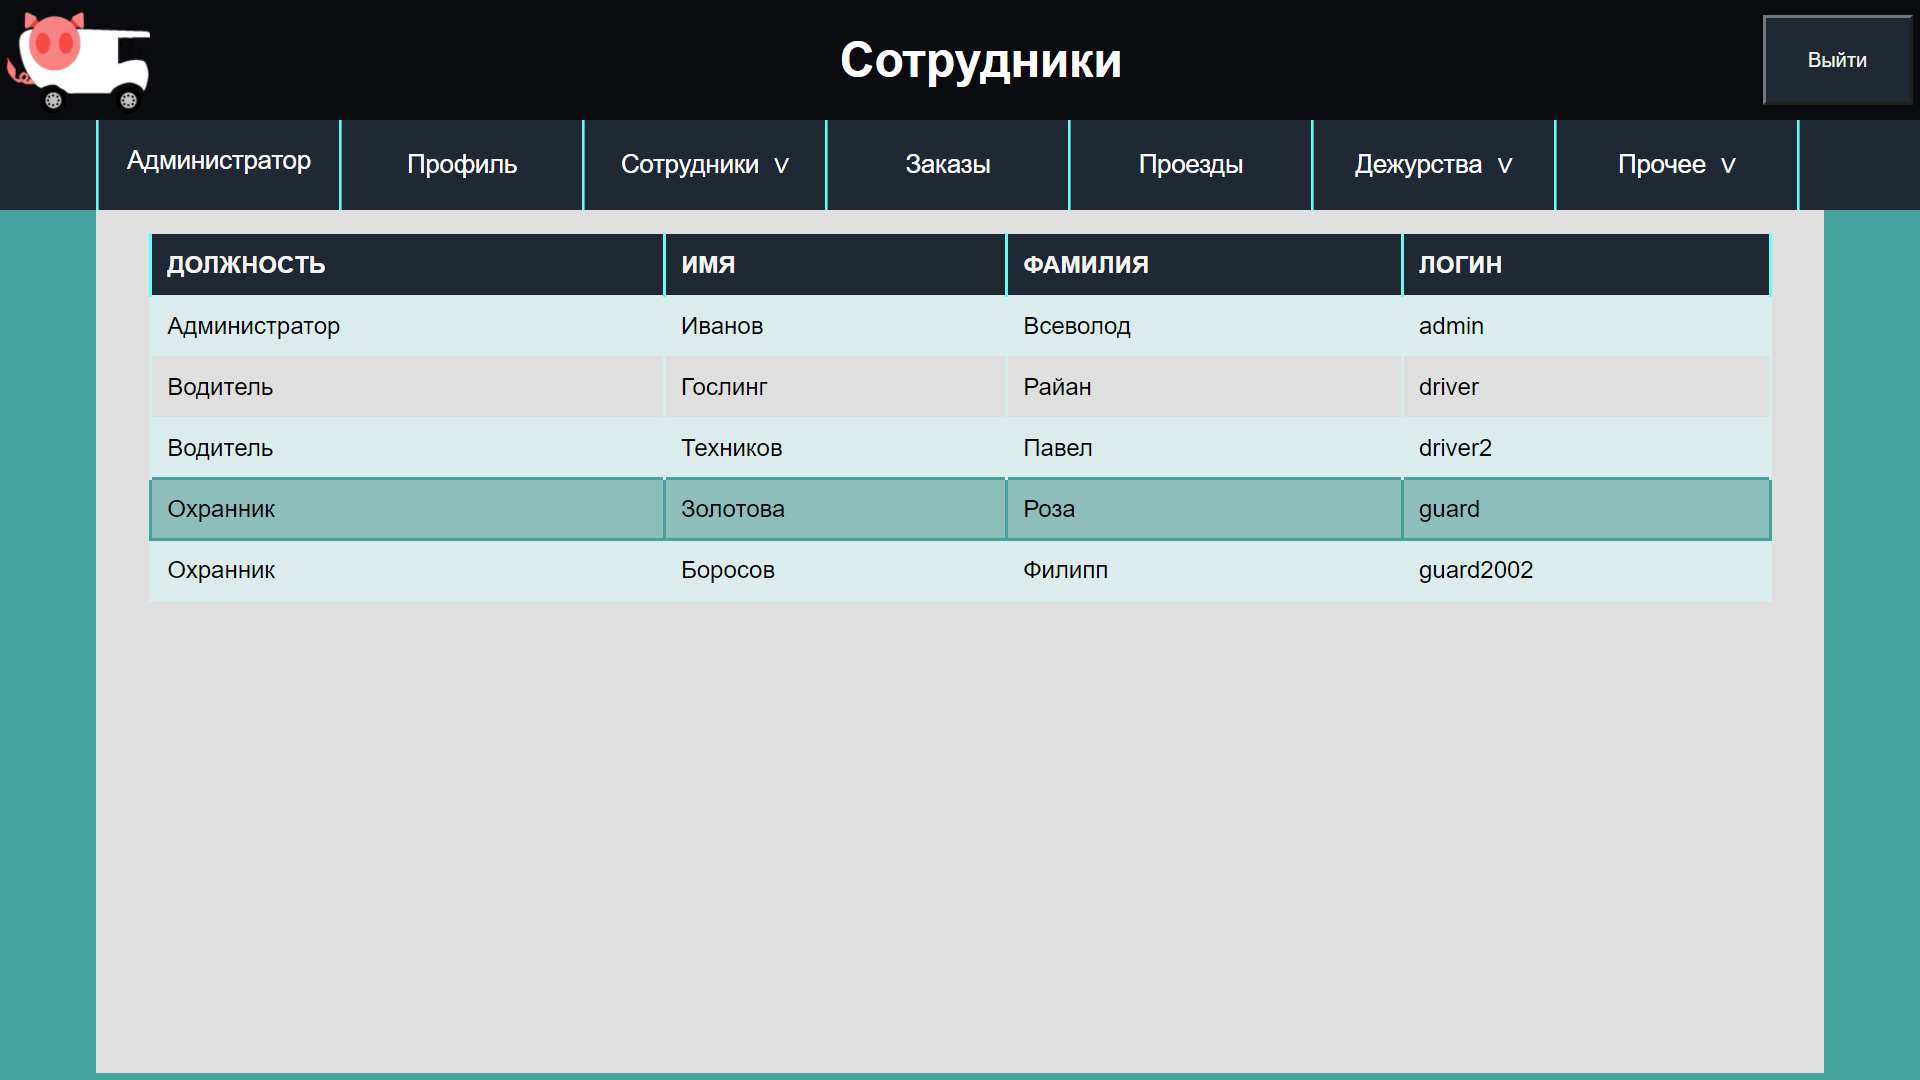
\includegraphics[scale=0.43, angle=0]{sc/all_profiles}}
		\caption{Страница просмотра всех сотрудников}
		\label{all_profiles_sc}
	\end{center}
\end{figure}

\begin{figure}[h!] 
	\begin{center}
		%		{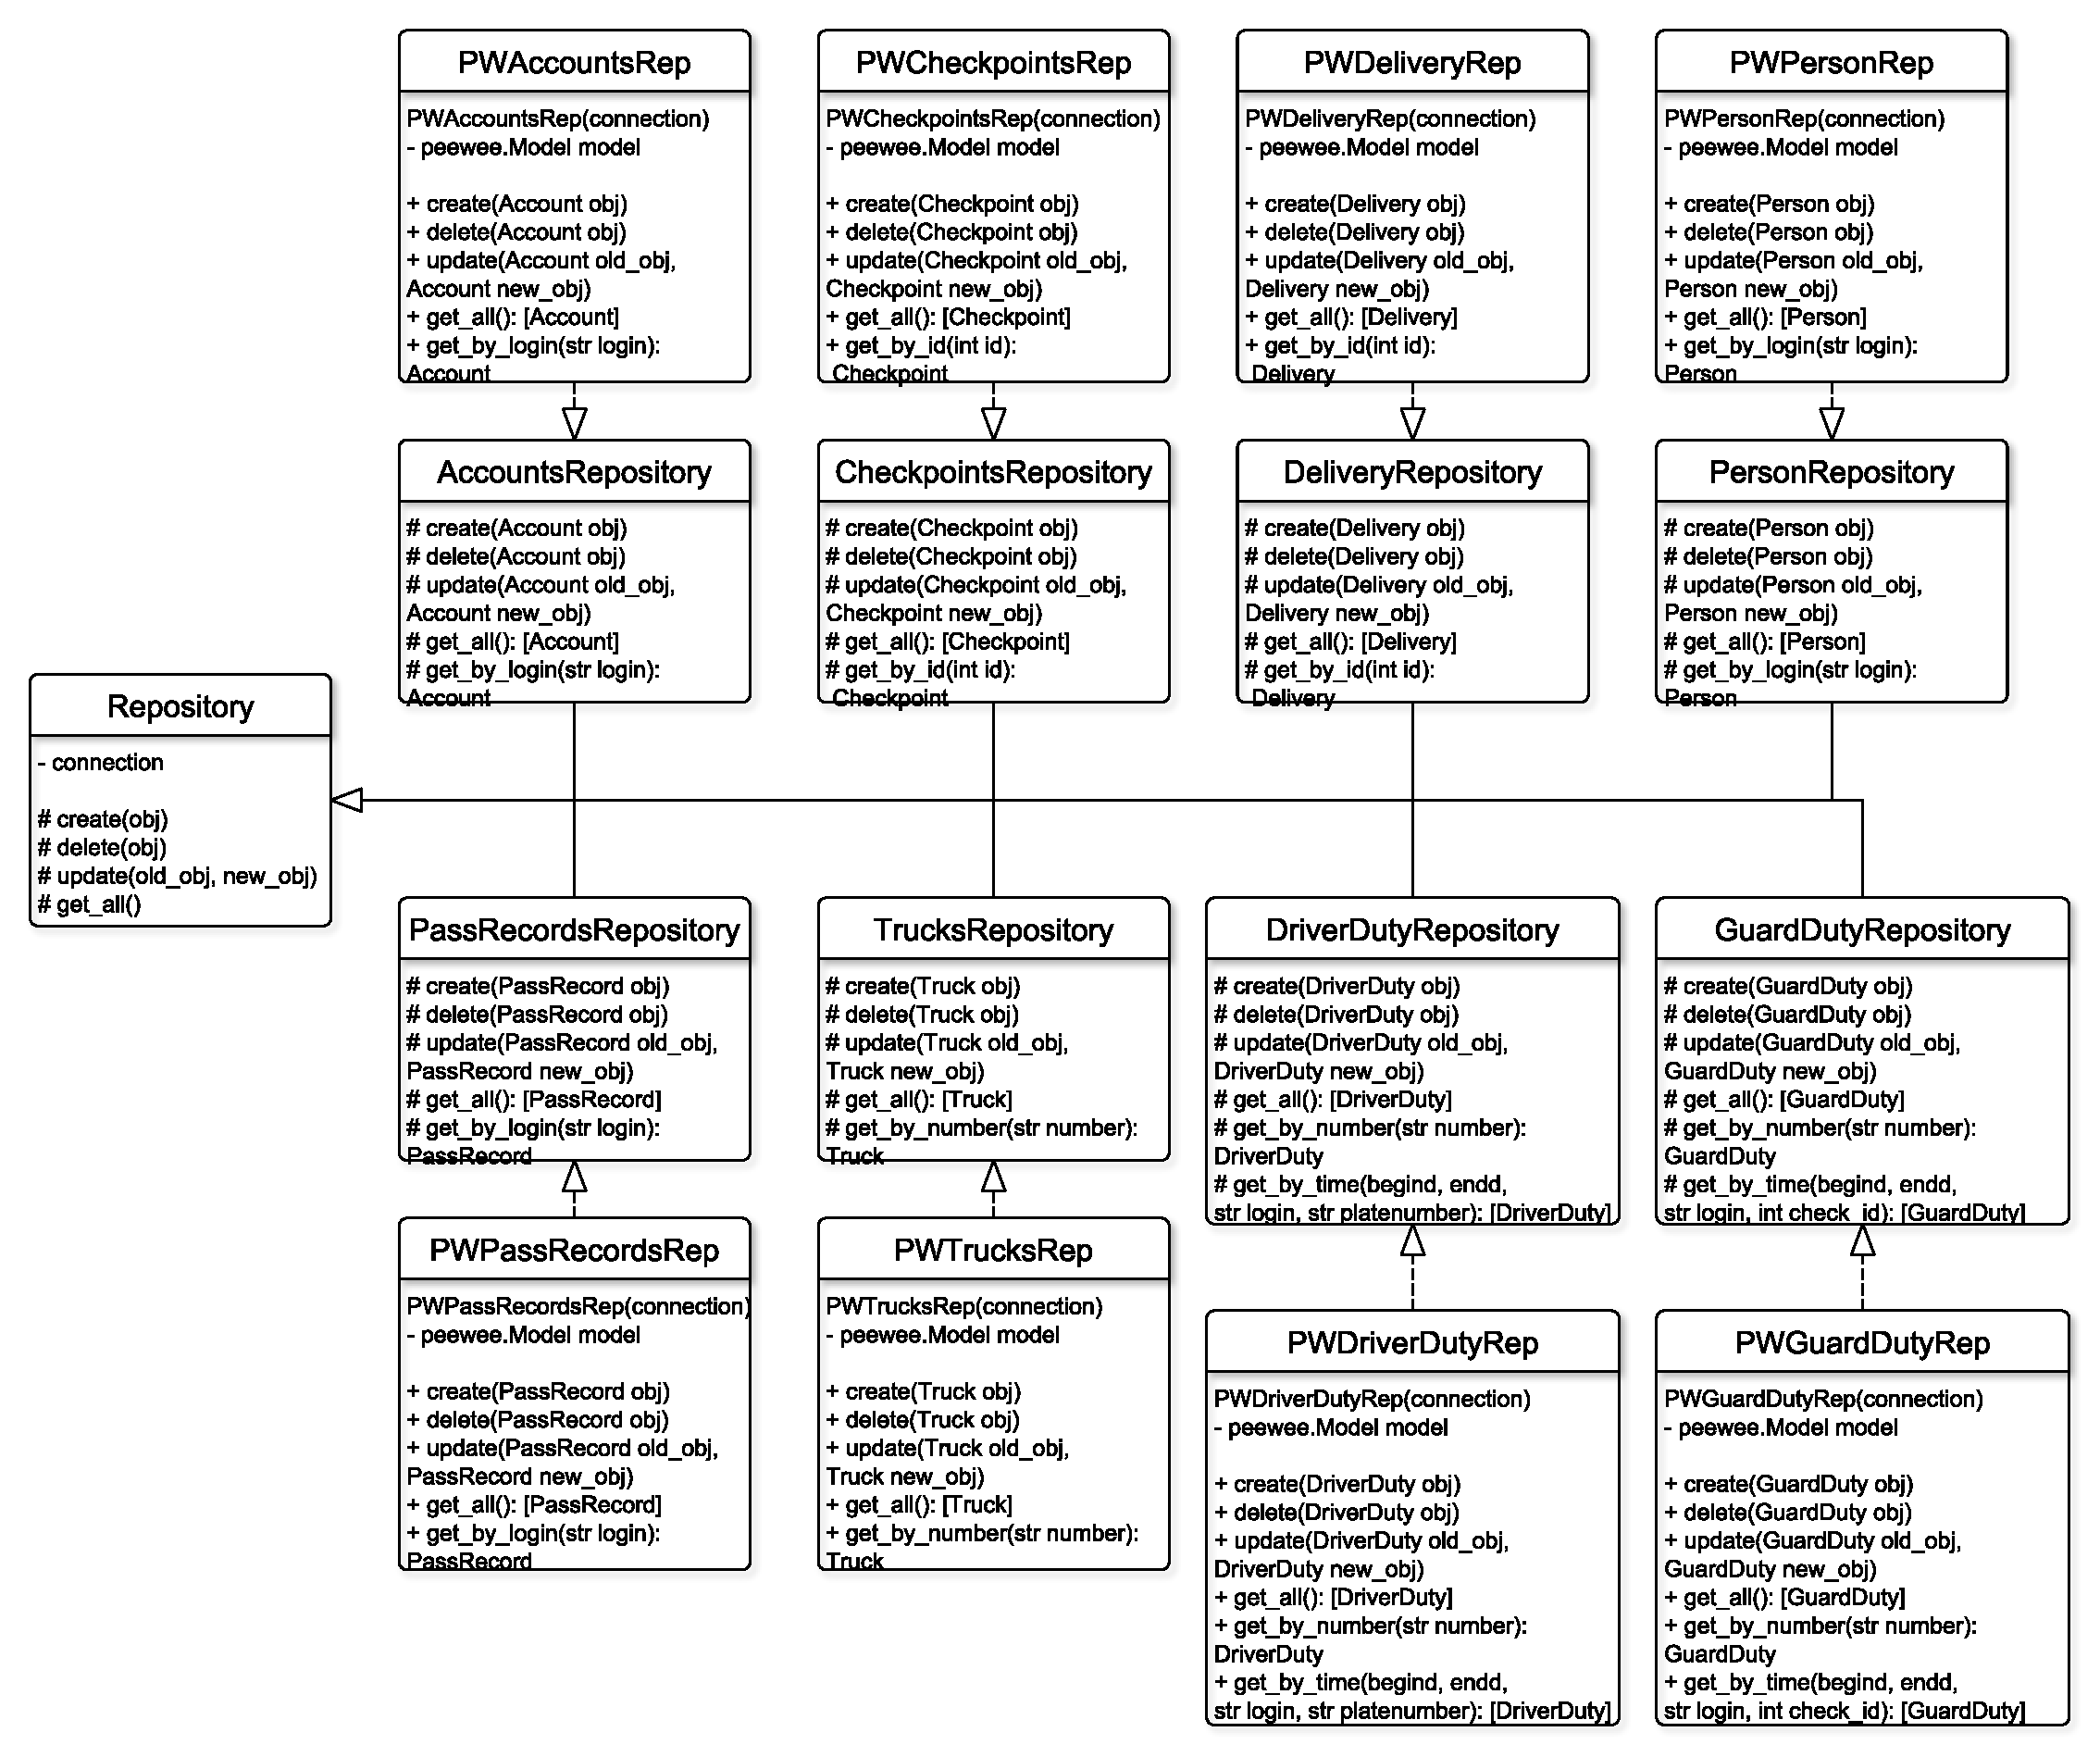
\includegraphics[height=14cm, width = 14cm]{uml/repsoitory.pdf}}
		{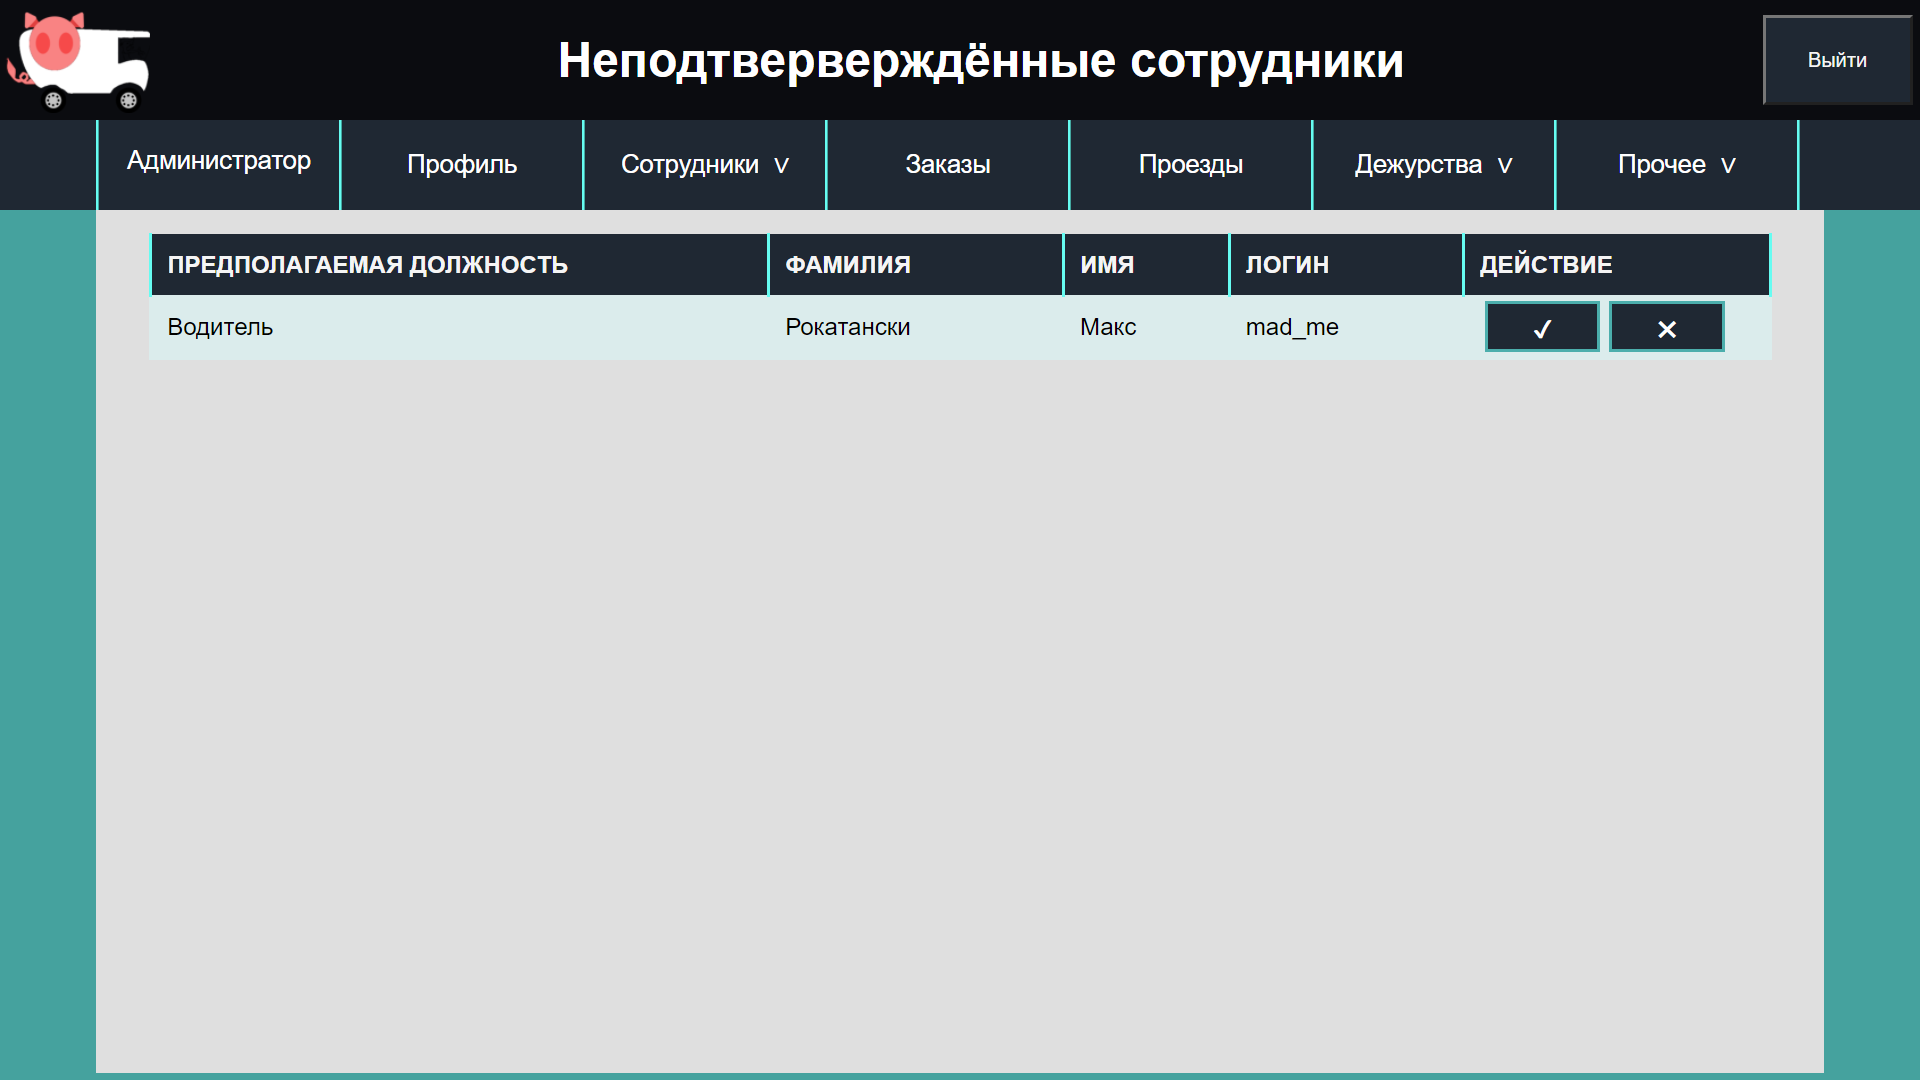
\includegraphics[scale=0.43, angle=0]{sc/unver}}
		\caption{Страница просмотра заявок регистрации}
		\label{unver_sc}
	\end{center}
\end{figure}

\begin{figure}[h!] 
	\begin{center}
		%		{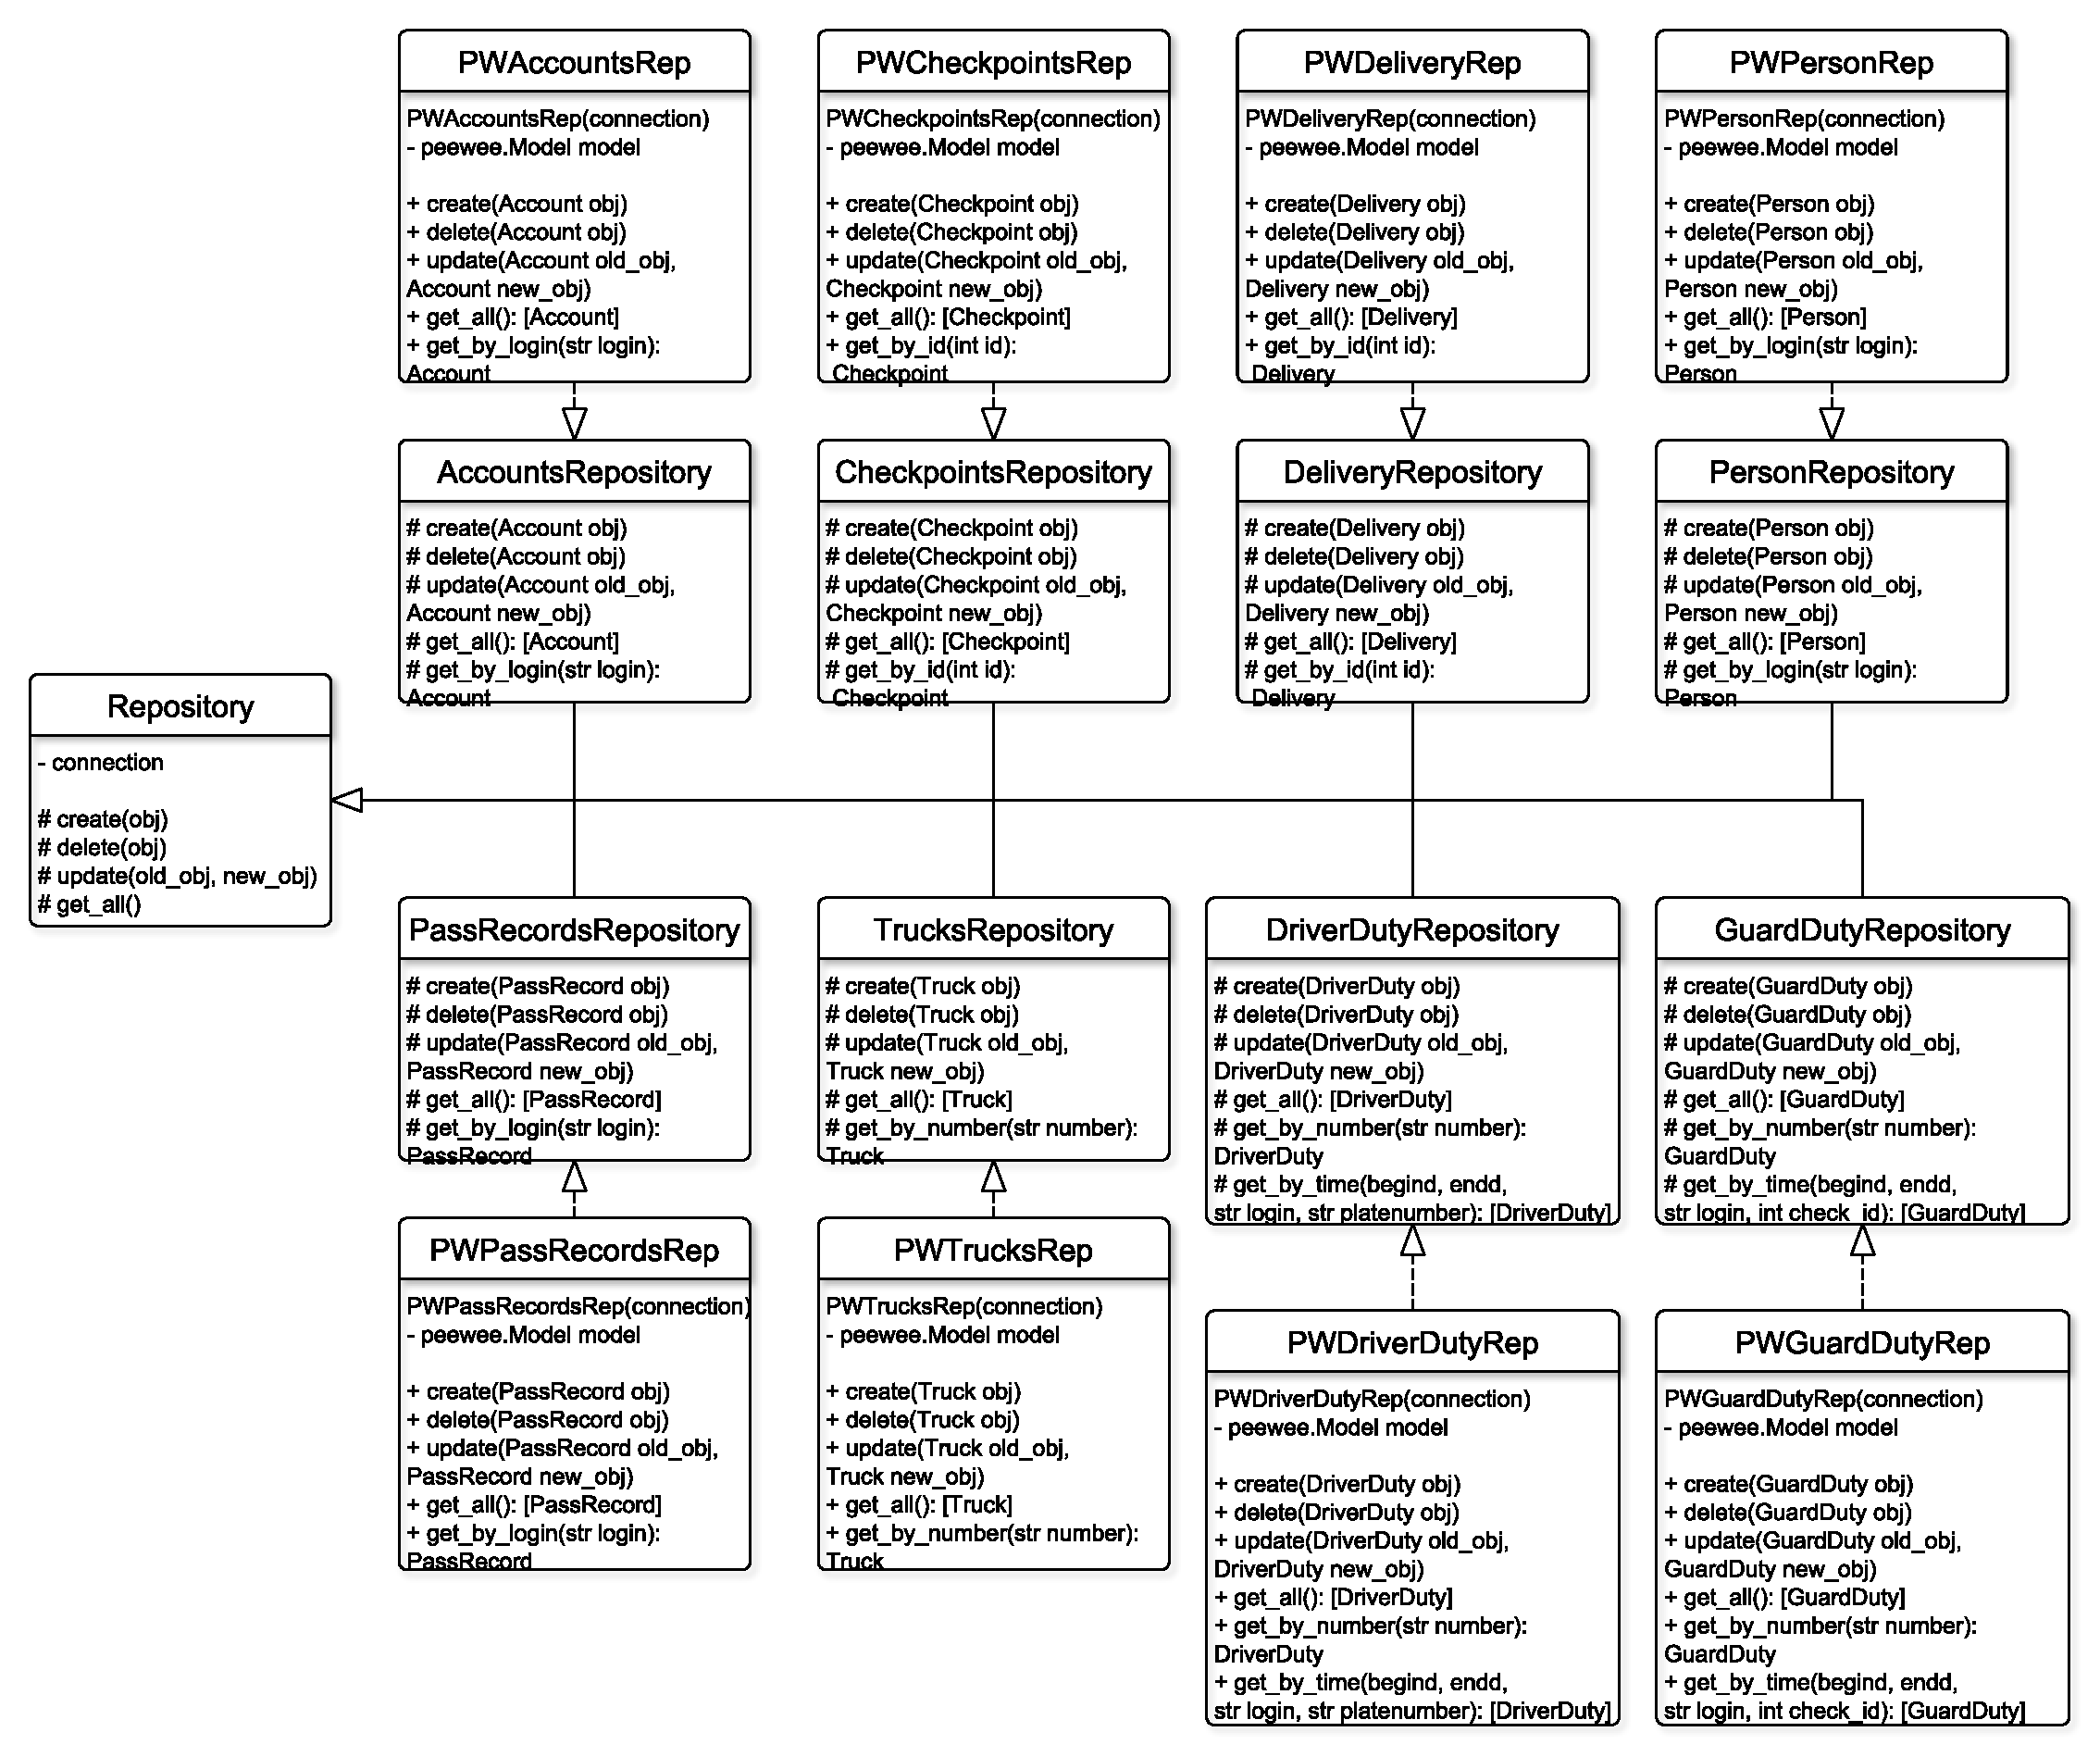
\includegraphics[height=14cm, width = 14cm]{uml/repsoitory.pdf}}
		{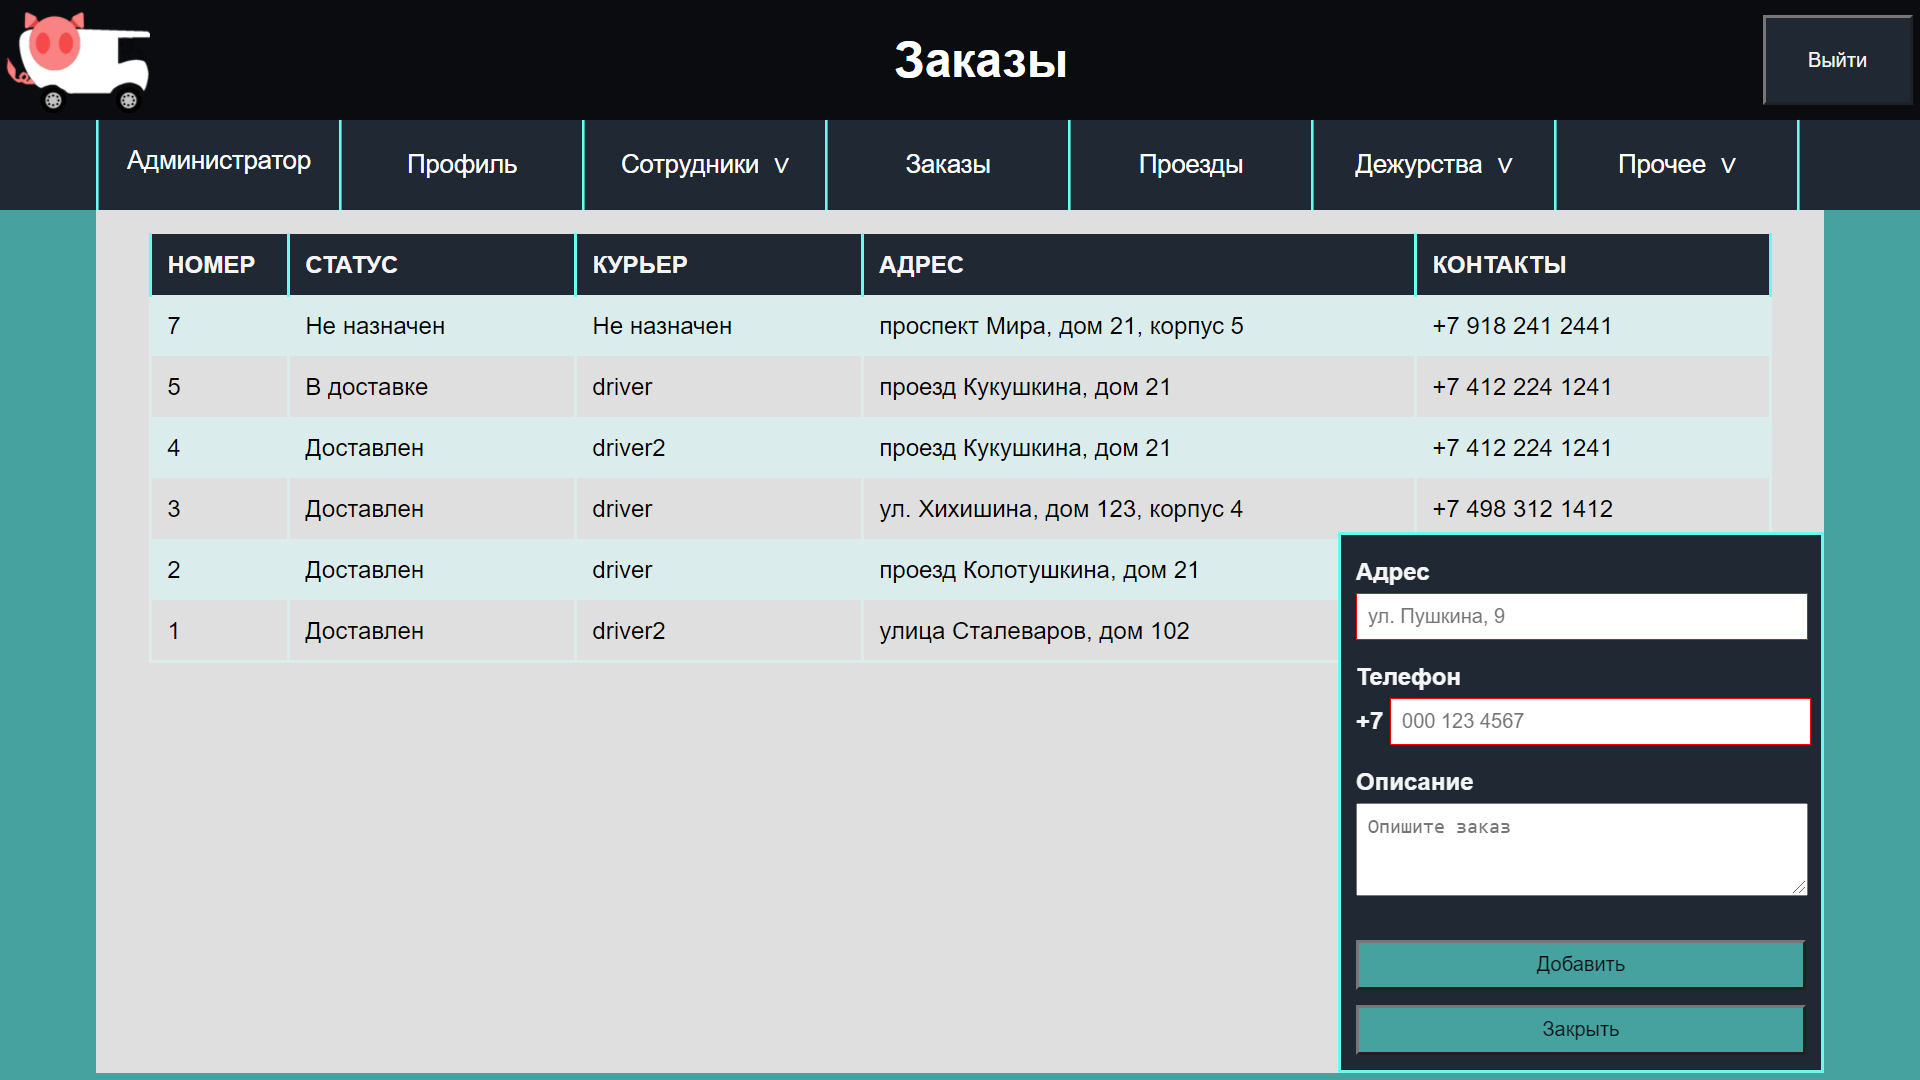
\includegraphics[scale=0.43, angle=0]{sc/all_delivery}}
		\caption{Страница просмотра и создания заказов}
		\label{all_delivery_sc}
	\end{center}
\end{figure}

\begin{figure}[h!] 
	\begin{center}
		%		{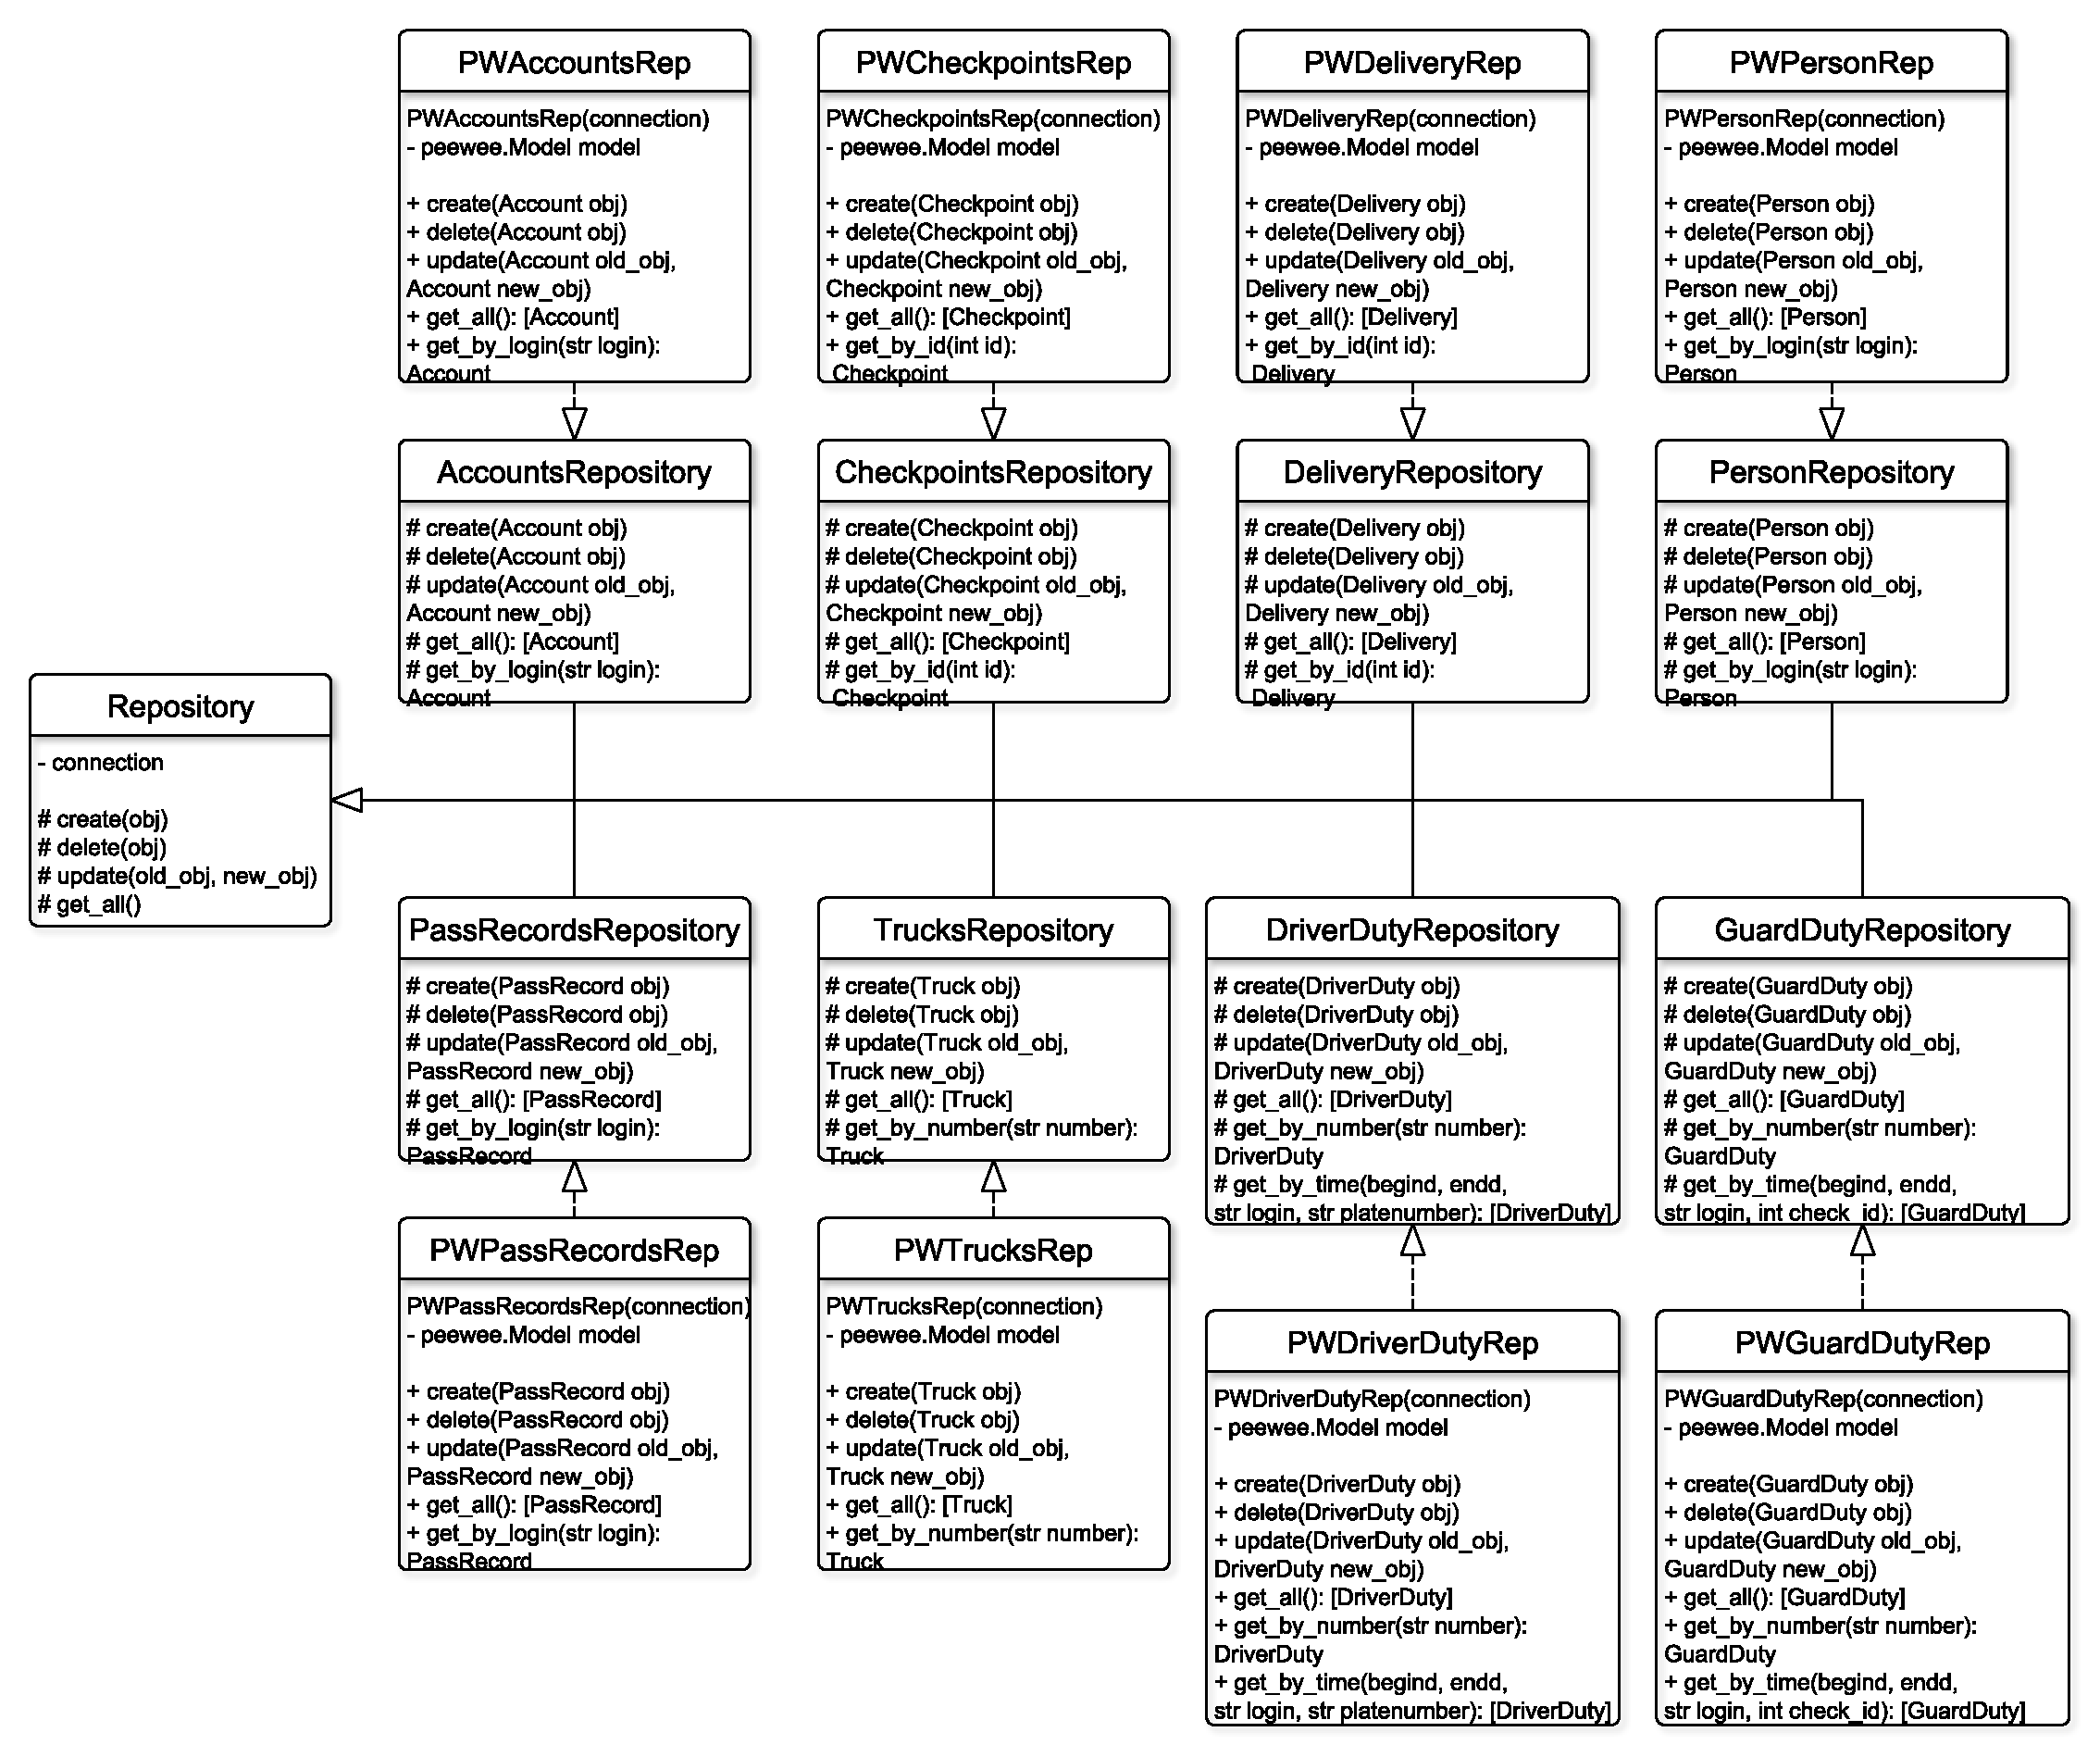
\includegraphics[height=14cm, width = 14cm]{uml/repsoitory.pdf}}
		{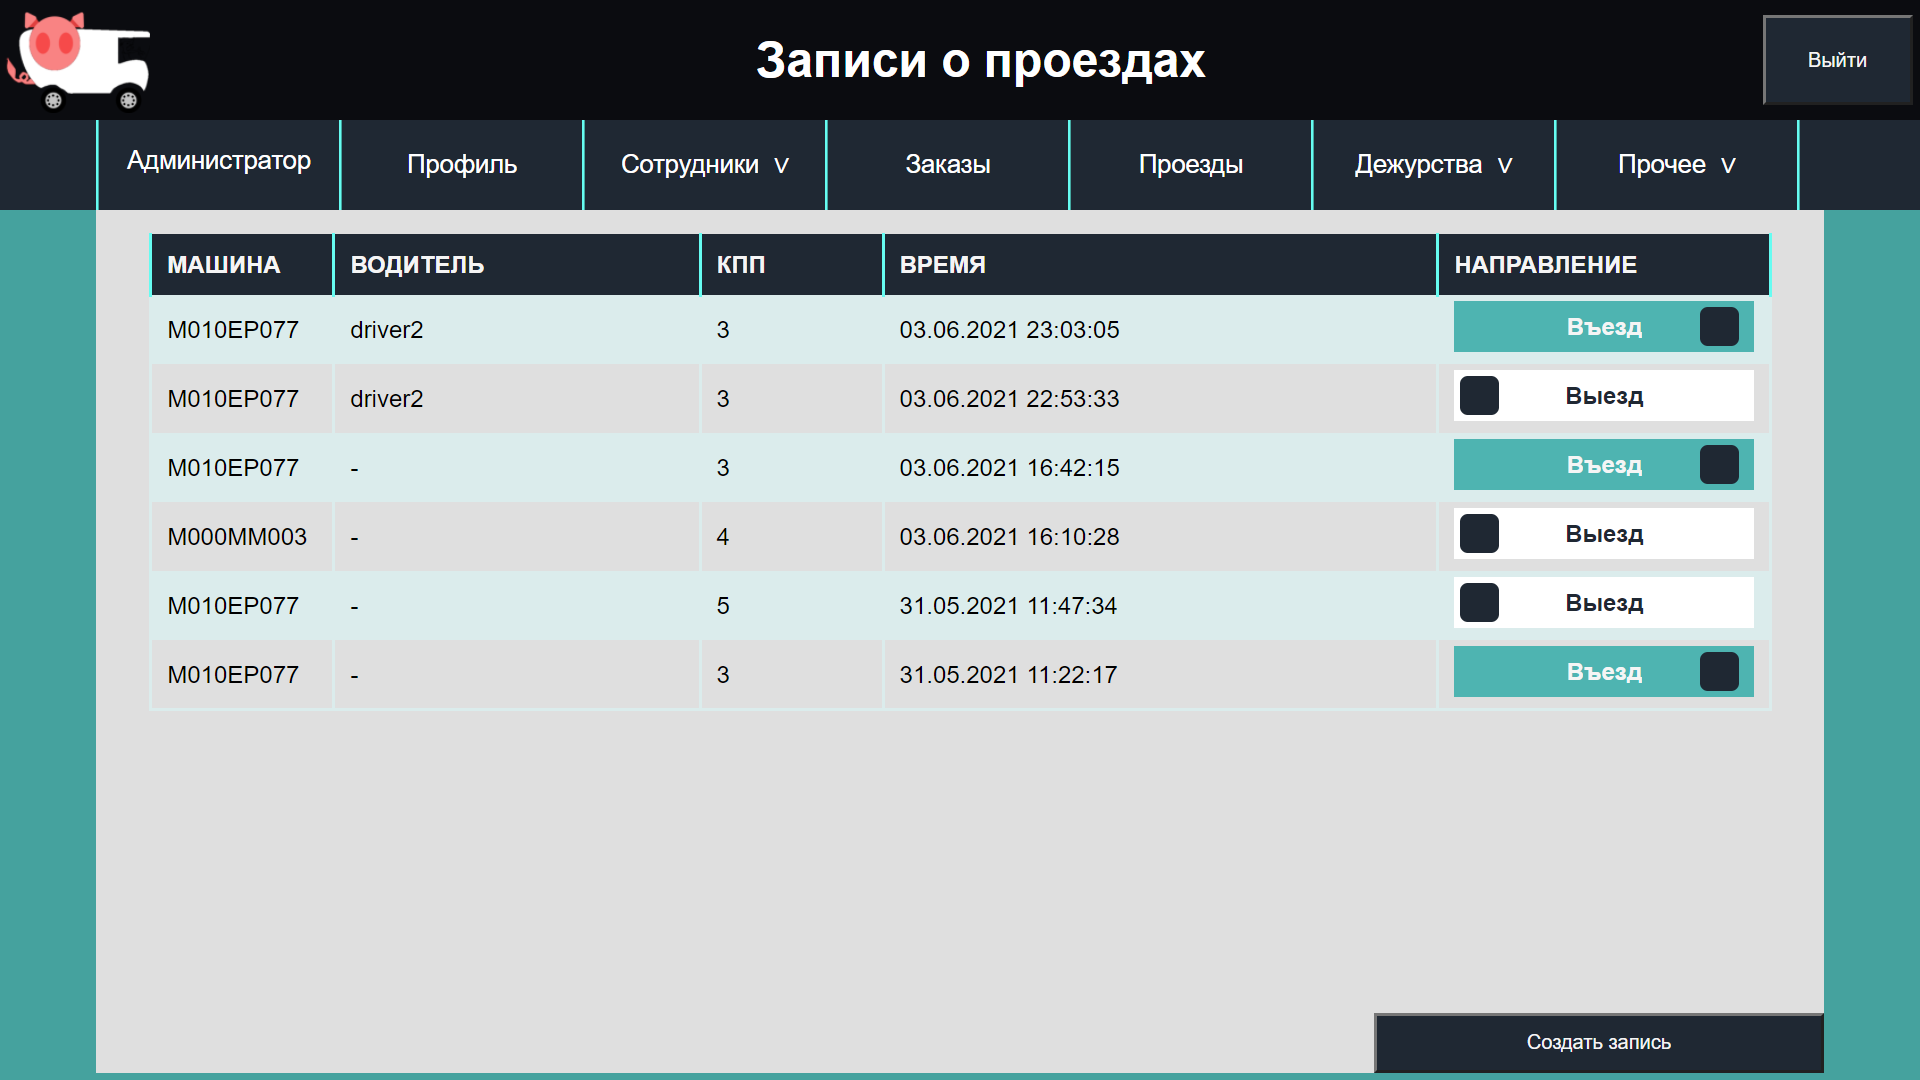
\includegraphics[scale=0.43, angle=0]{sc/all_pass}}
		\caption{Страница просмотра и регистрации записей о проездах}
		\label{all_pass_sc}
	\end{center}
\end{figure}

\begin{figure}[h!] 
	\begin{center}
		%		{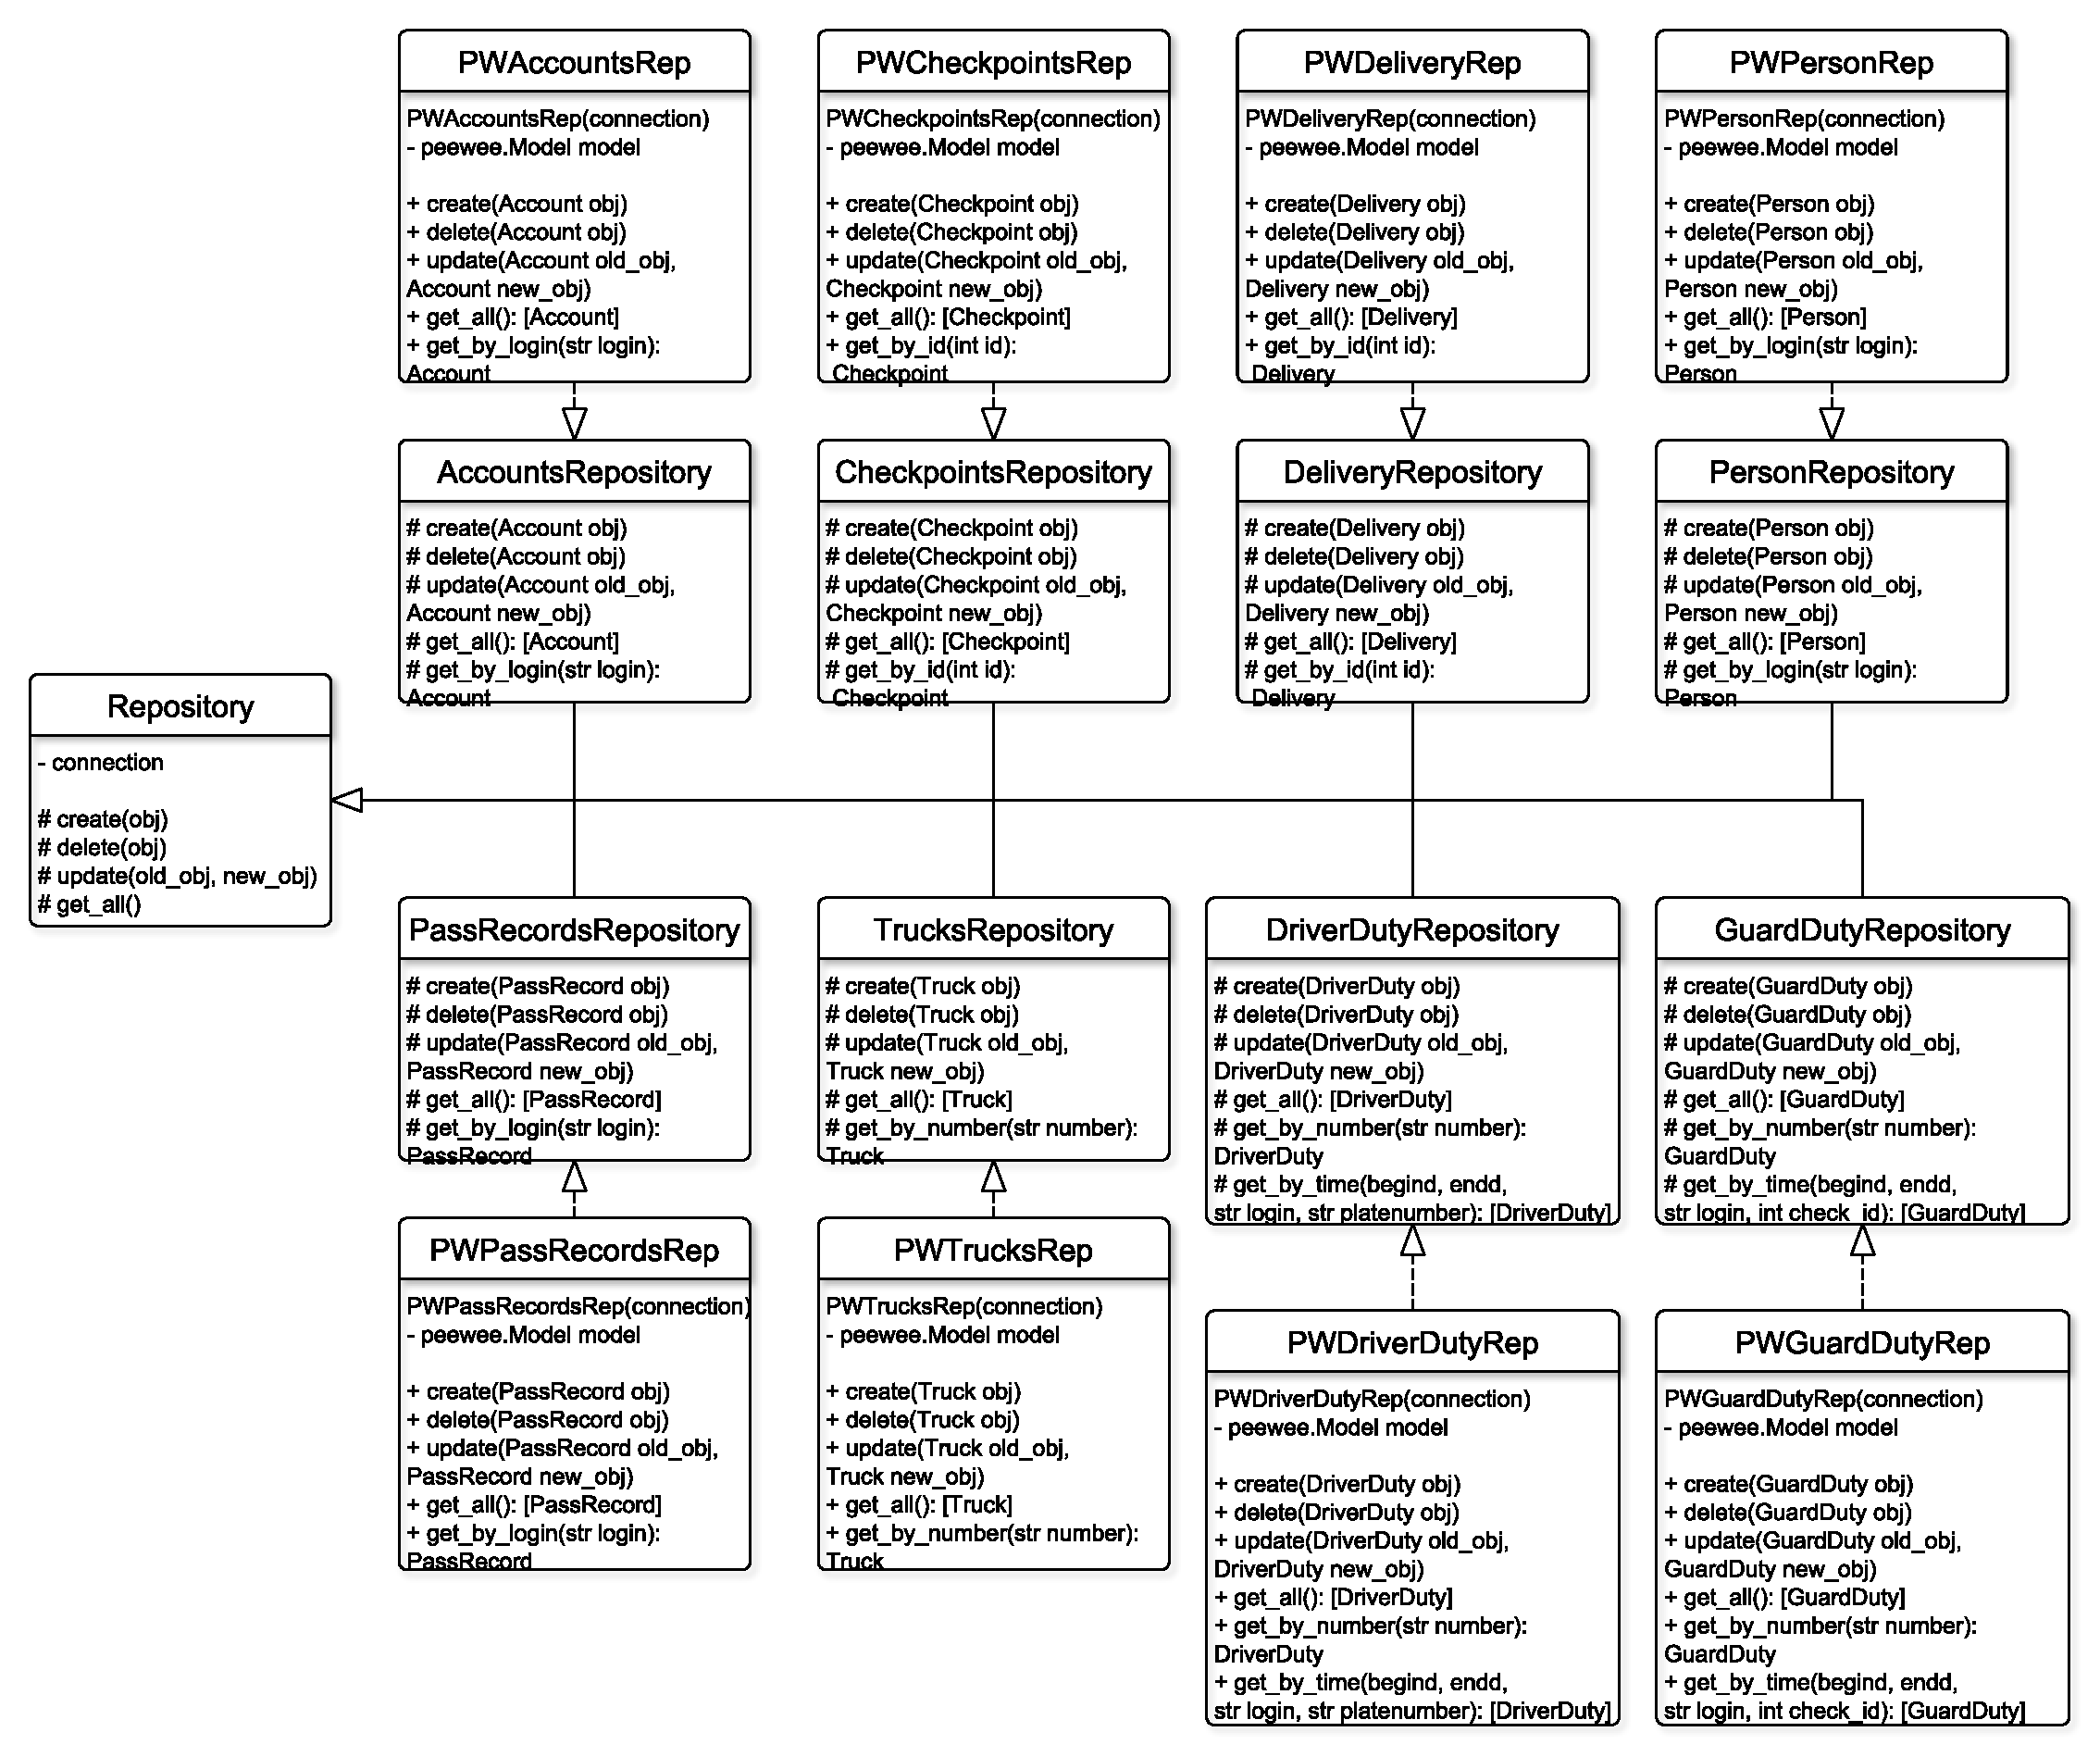
\includegraphics[height=14cm, width = 14cm]{uml/repsoitory.pdf}}
		{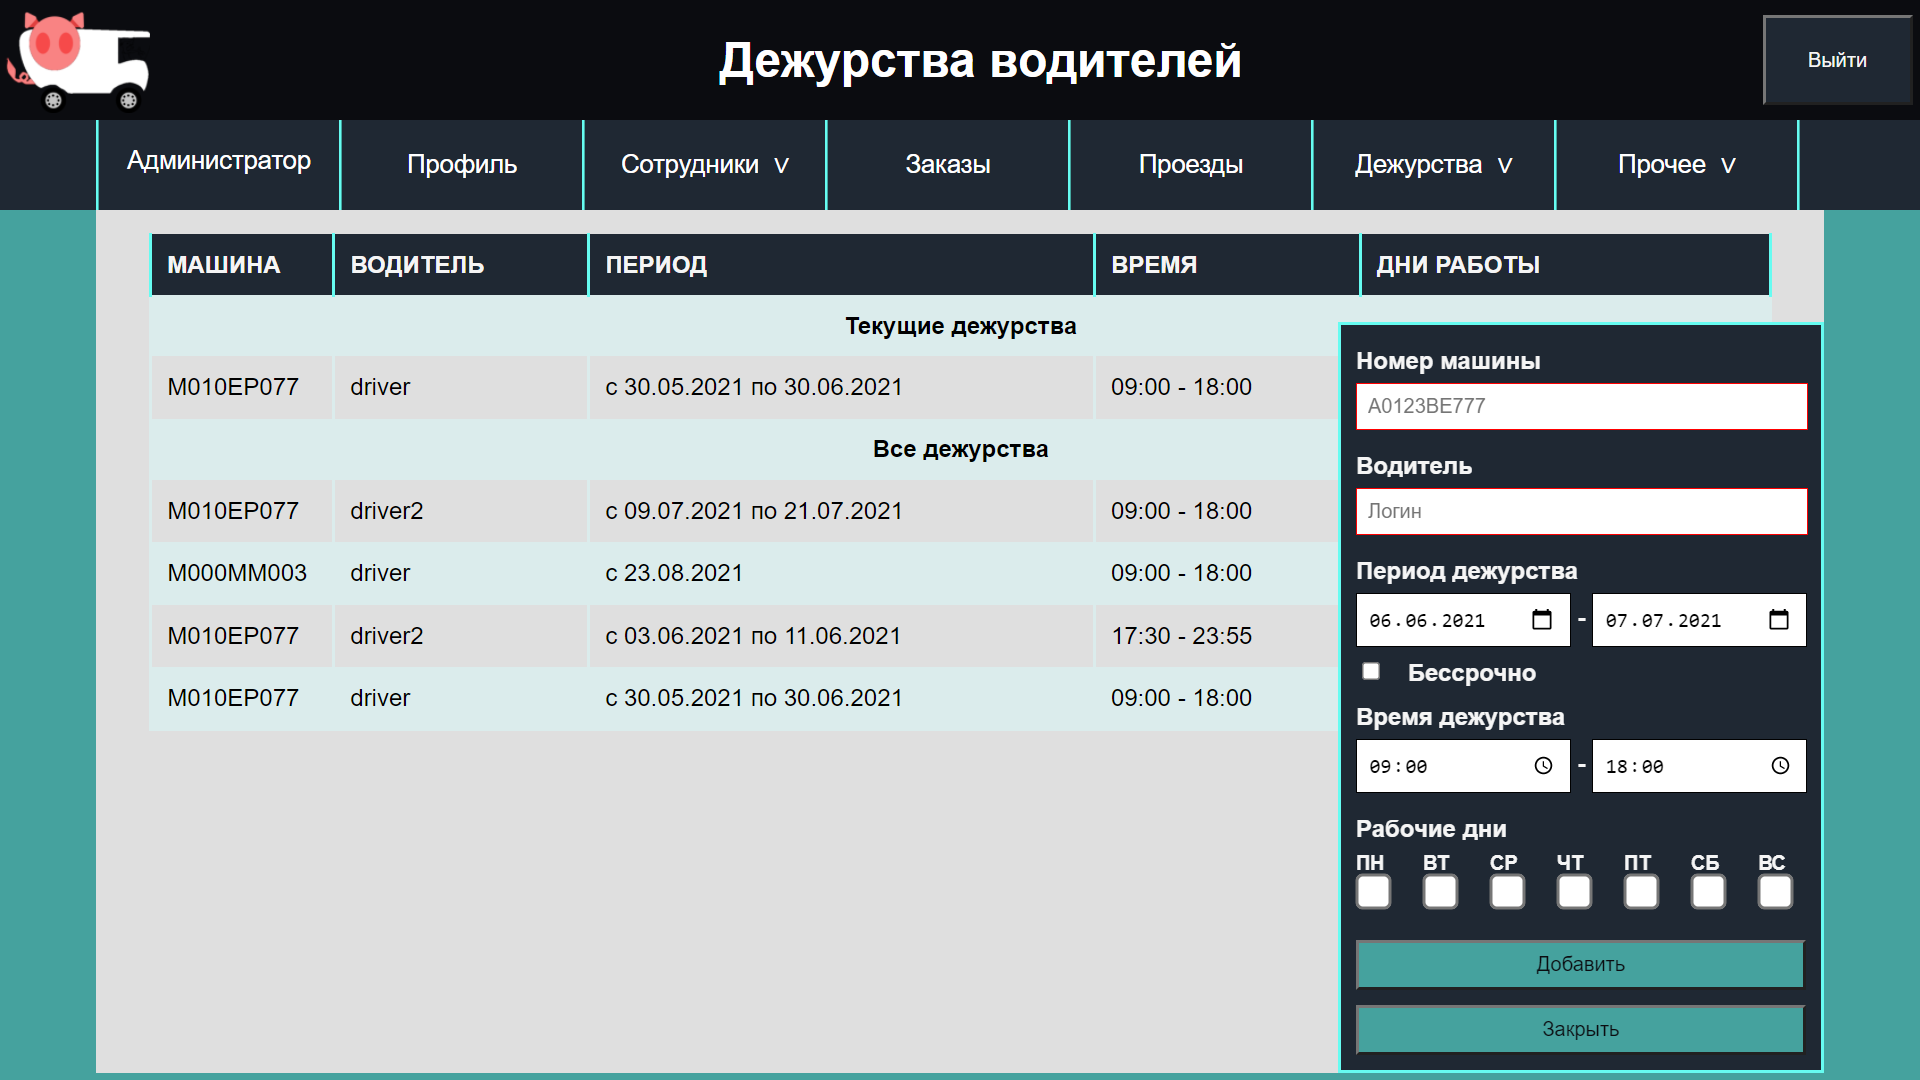
\includegraphics[scale=0.43, angle=0]{sc/driver_duty}}
		\caption{Страница просмотра и назначения дежурств водителей}
		\label{driver_duty_sc}
	\end{center}
\end{figure}

\begin{figure}[h!] 
	\begin{center}
		%		{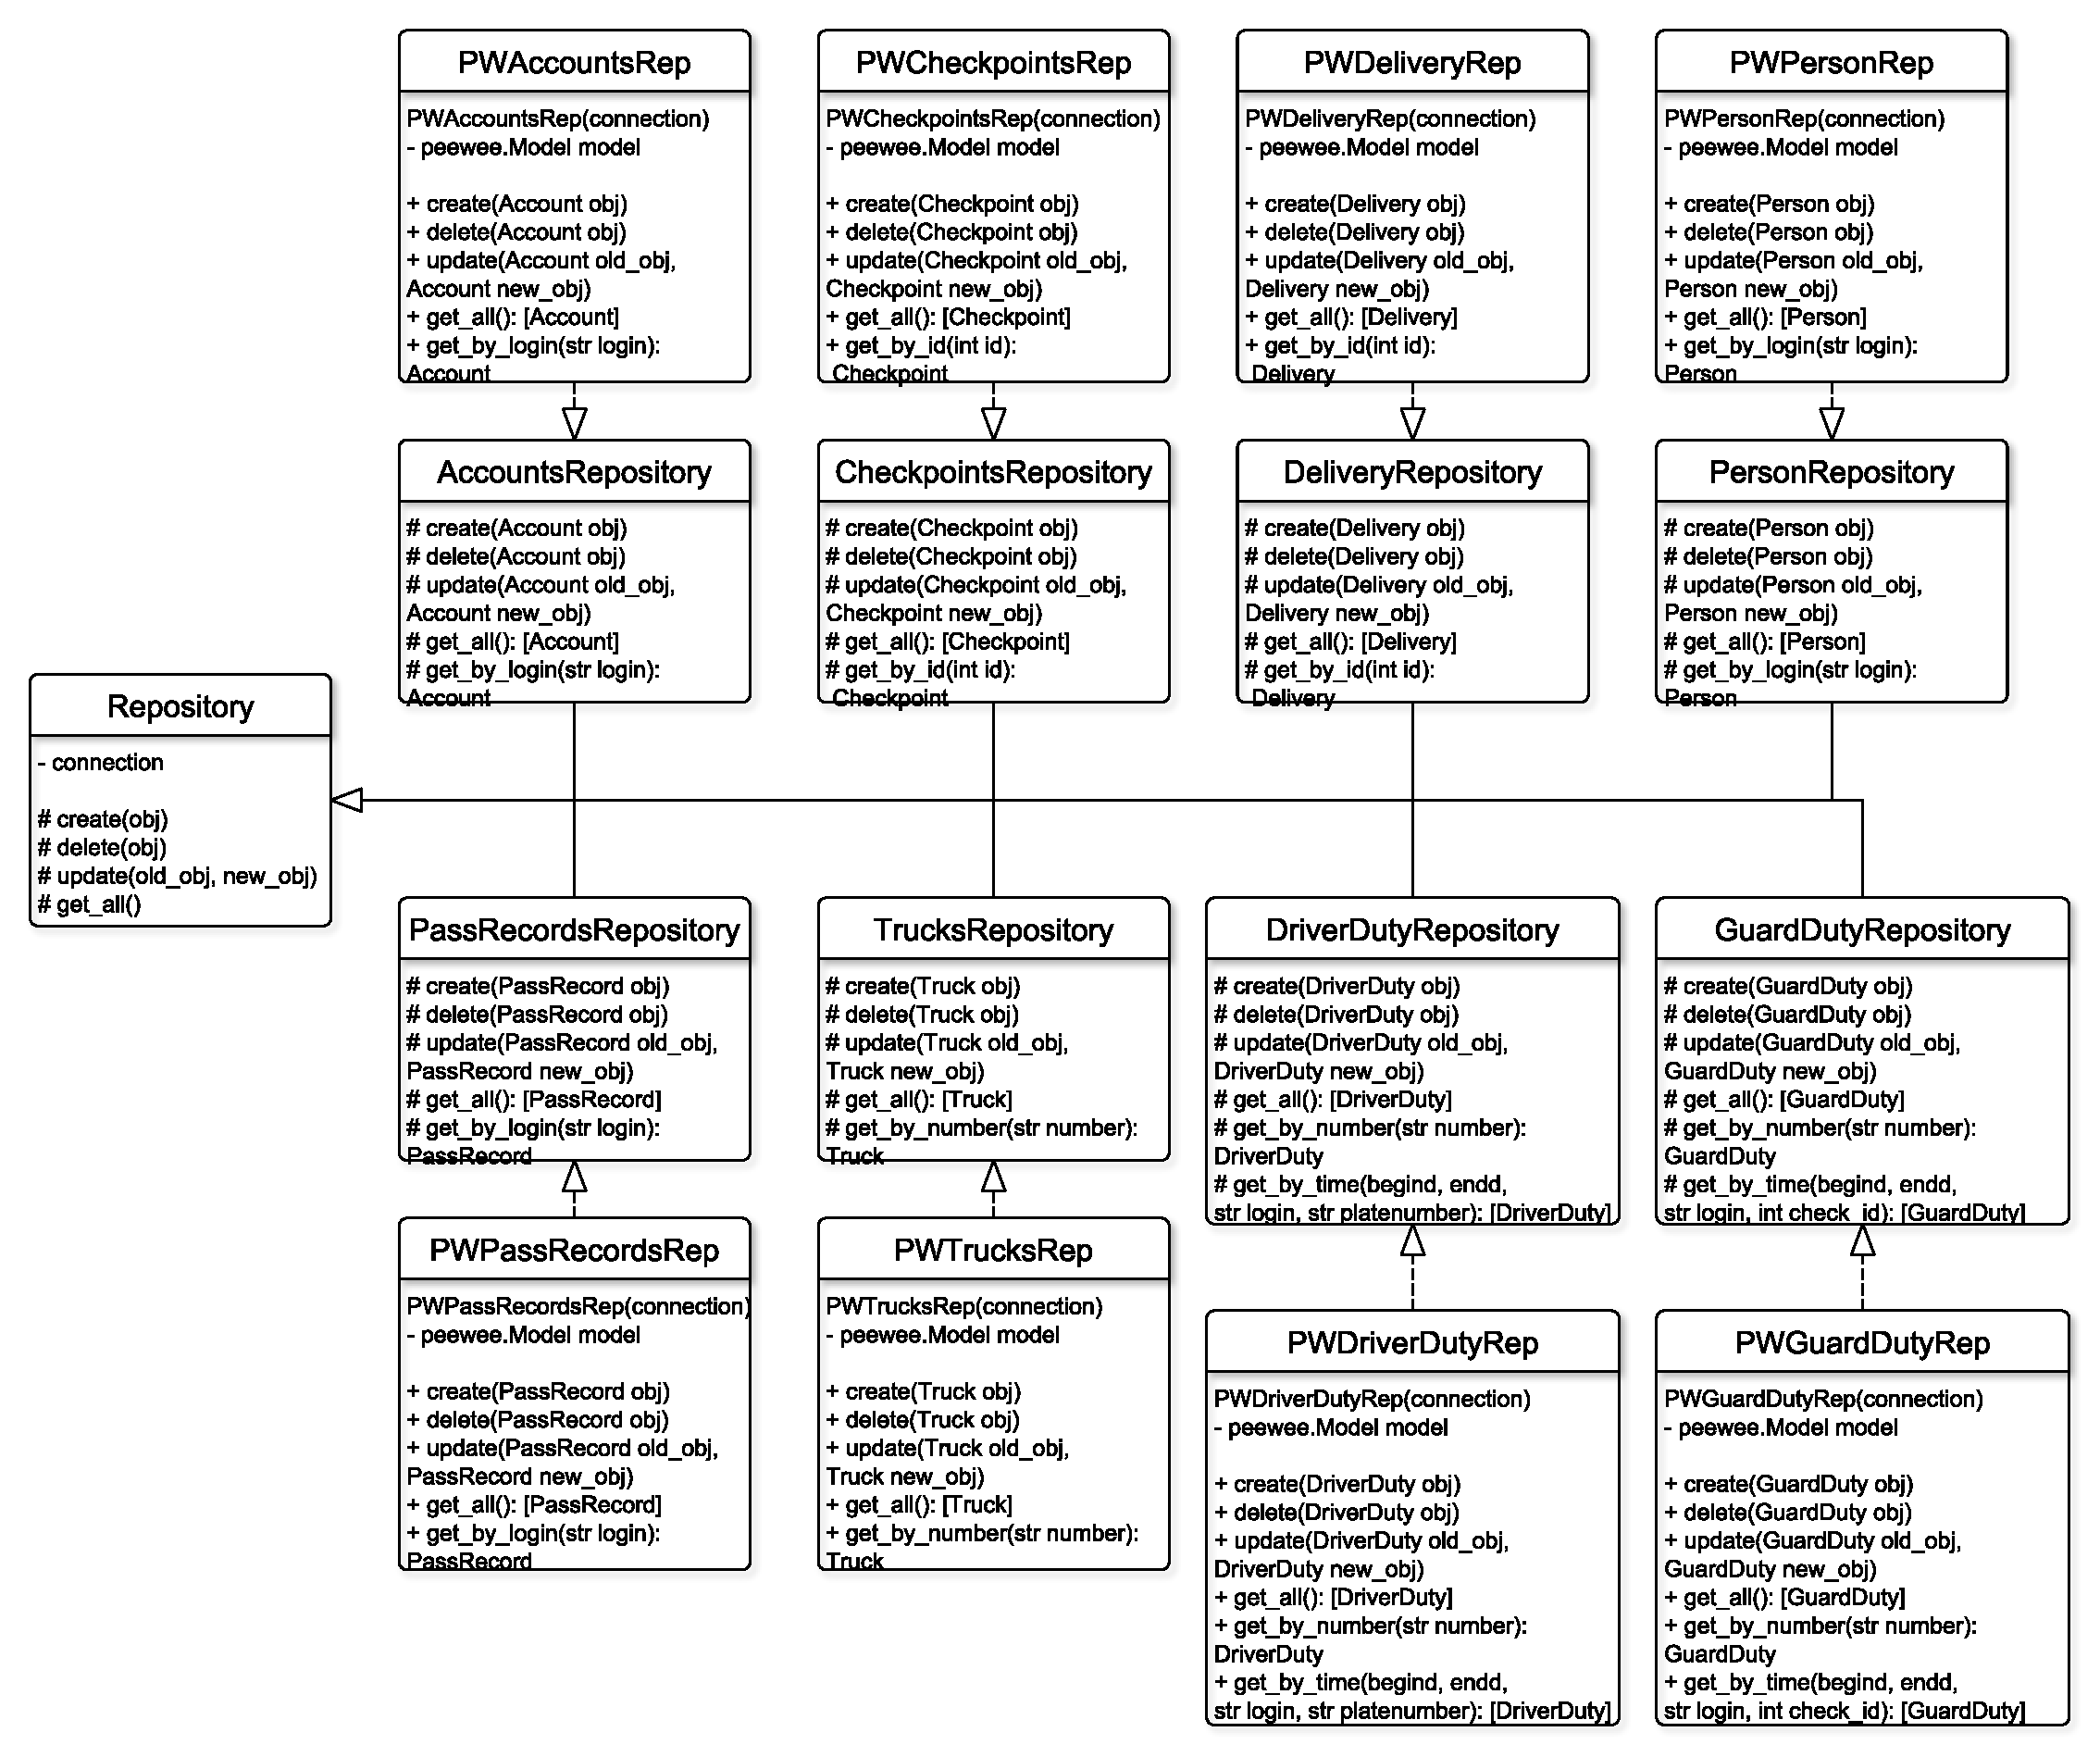
\includegraphics[height=14cm, width = 14cm]{uml/repsoitory.pdf}}
		{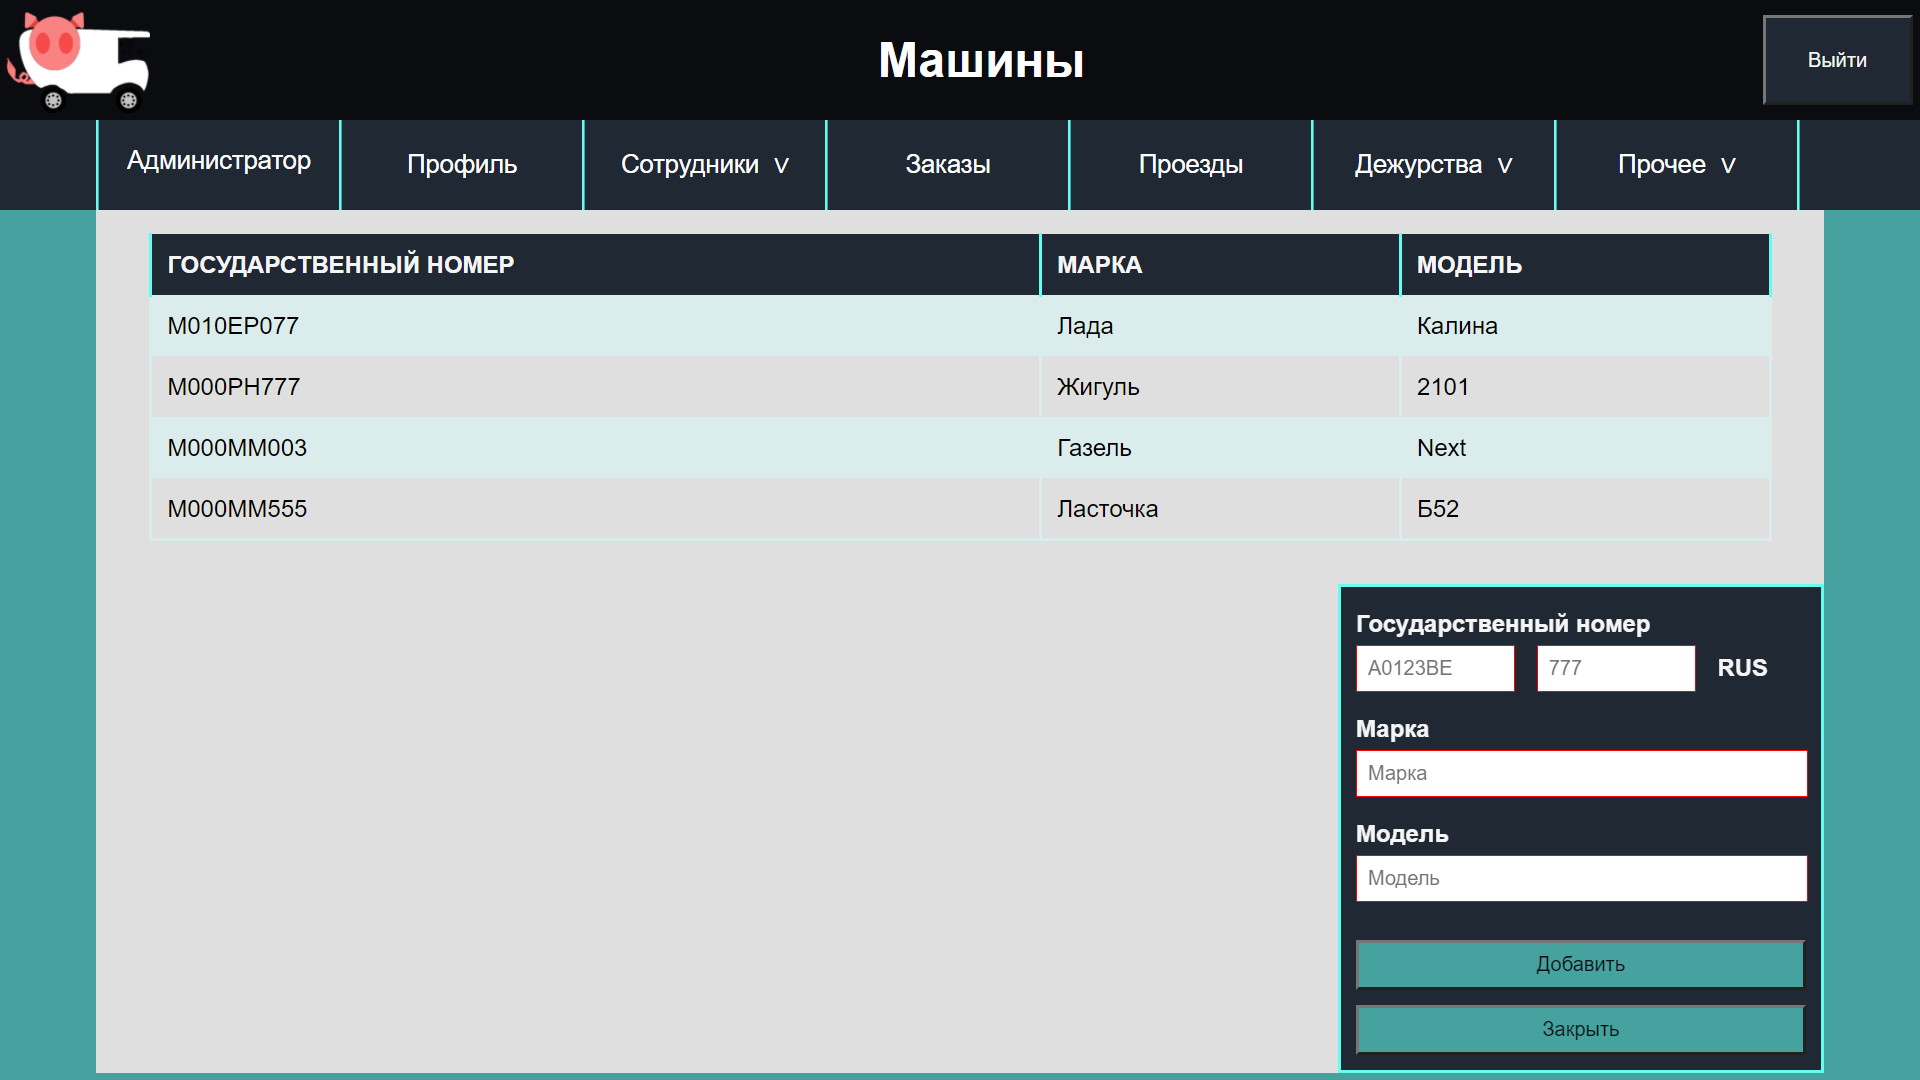
\includegraphics[scale=0.43, angle=0]{sc/trucks}}
		\caption{Страница просмотра и регистрации машин}
		\label{trucks_sc}
	\end{center}
\end{figure}

\begin{figure}[h!] 
	\begin{center}
		%		{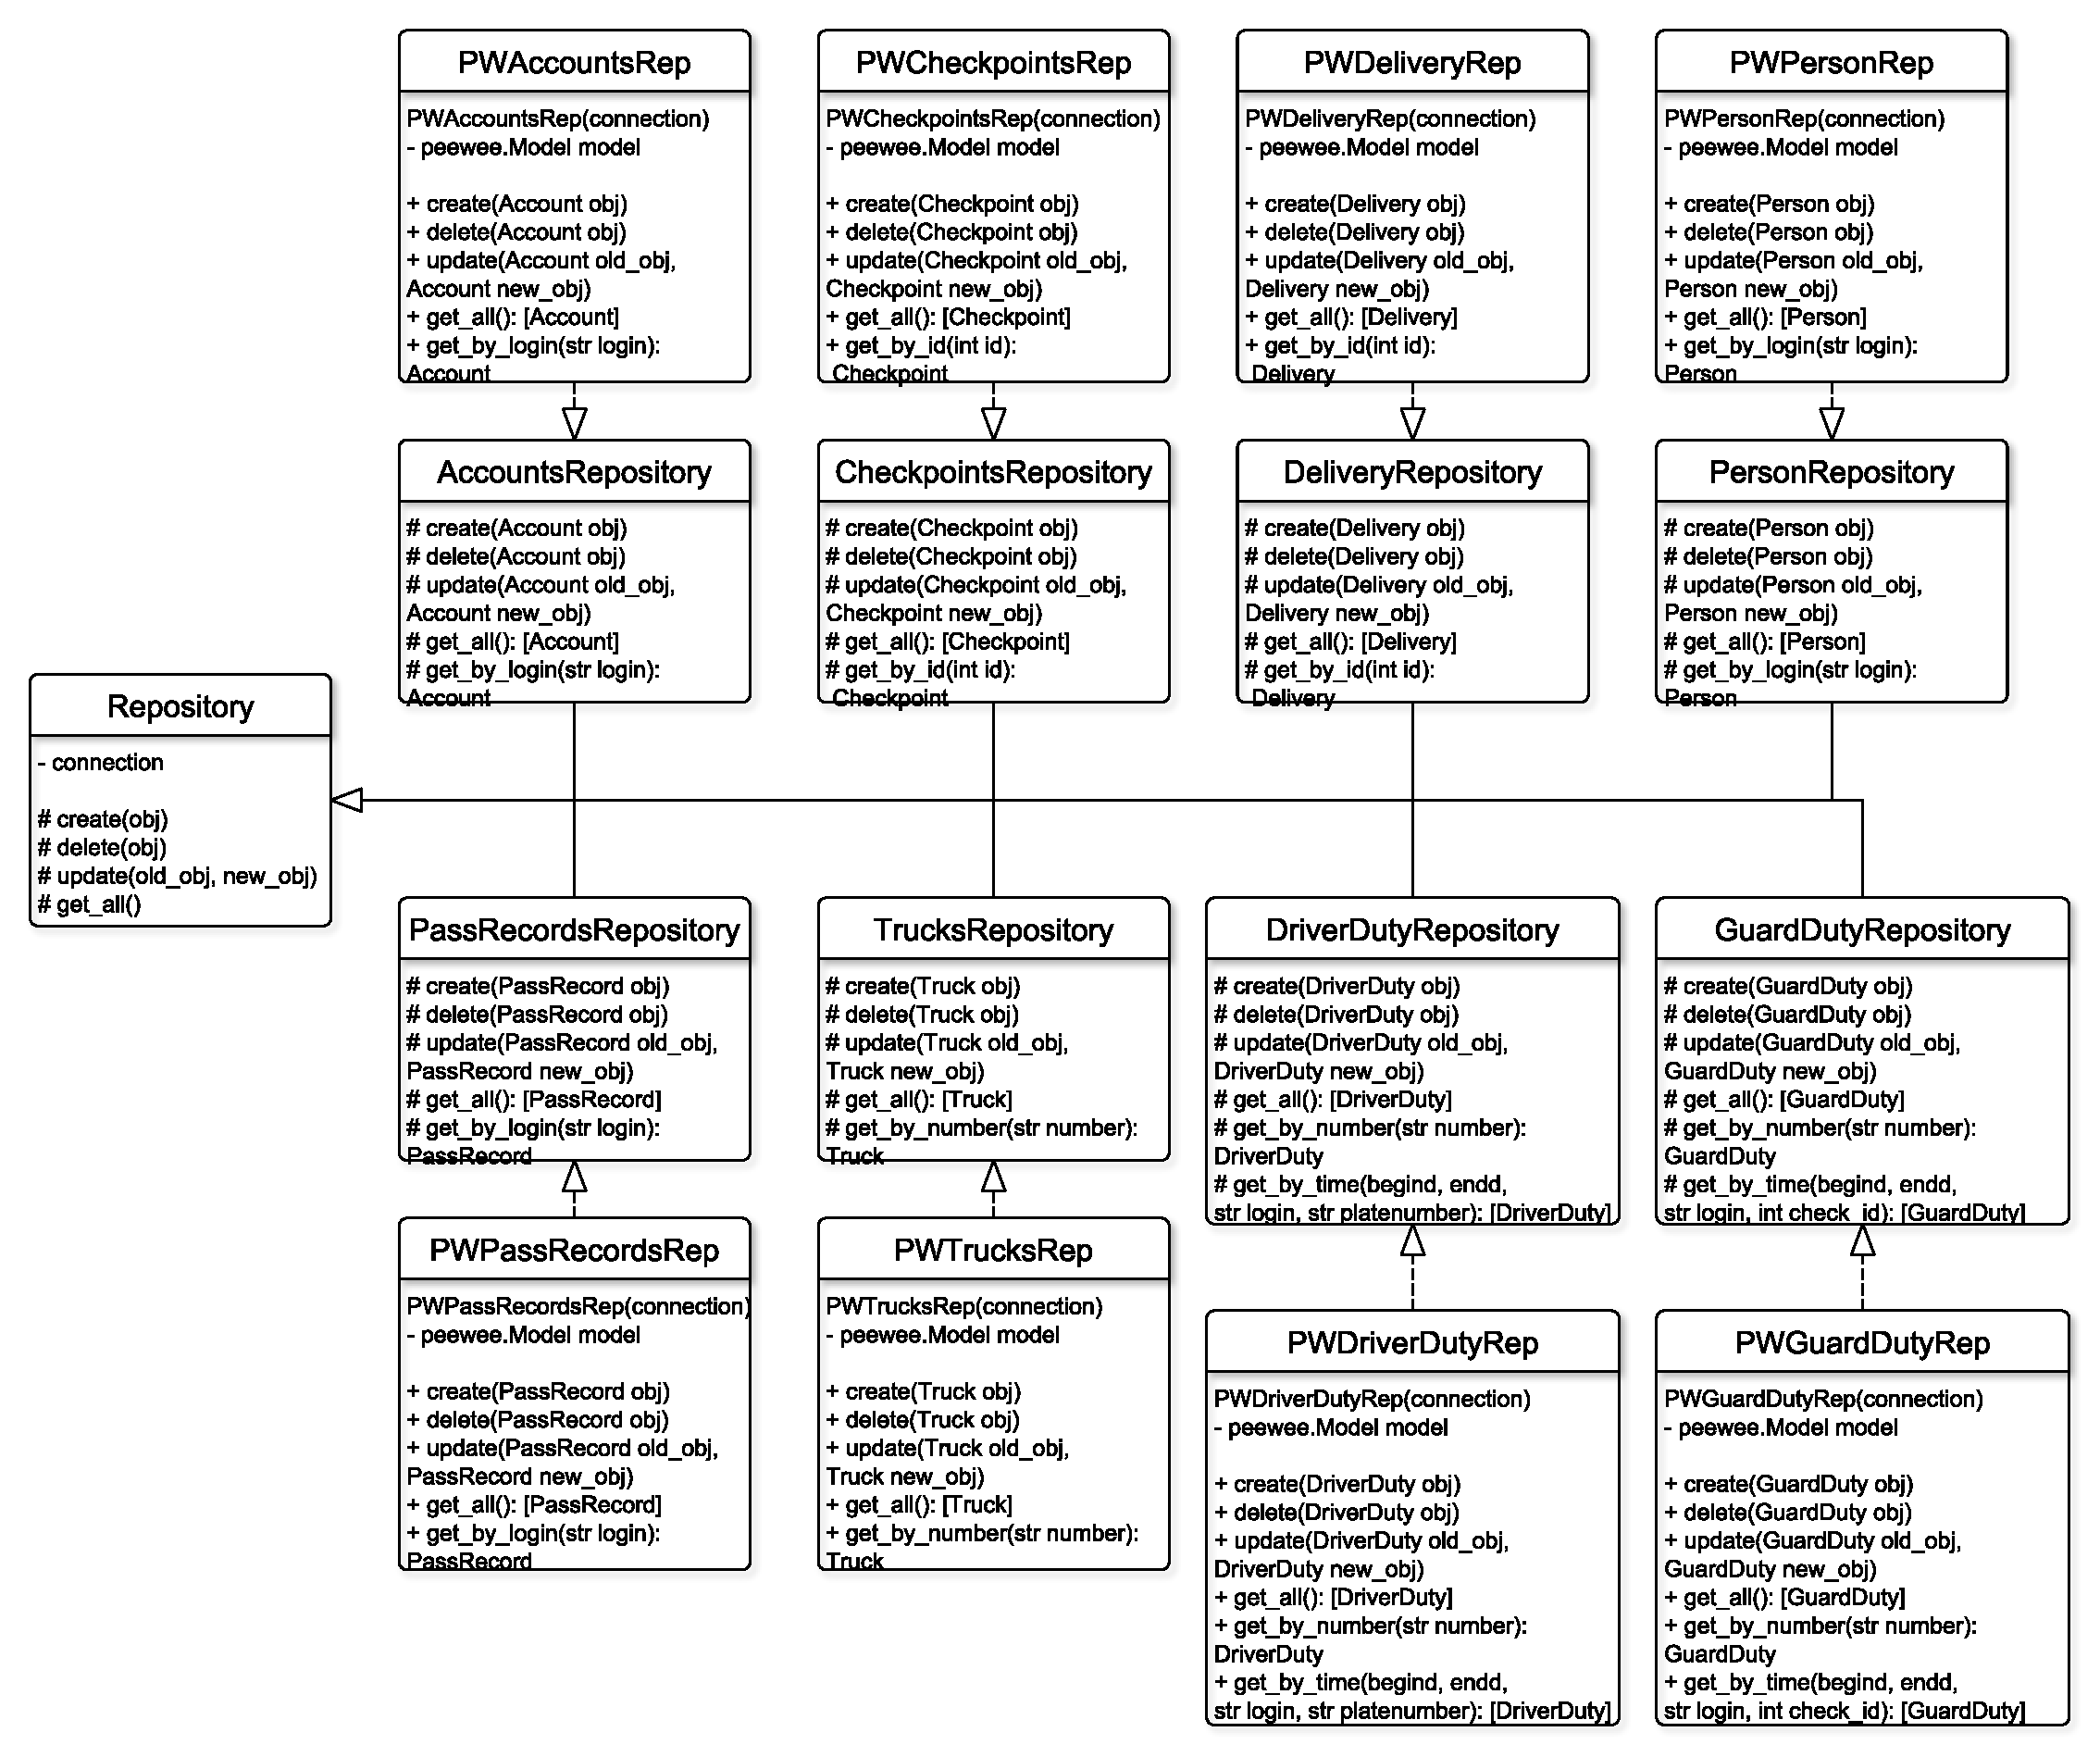
\includegraphics[height=14cm, width = 14cm]{uml/repsoitory.pdf}}
		{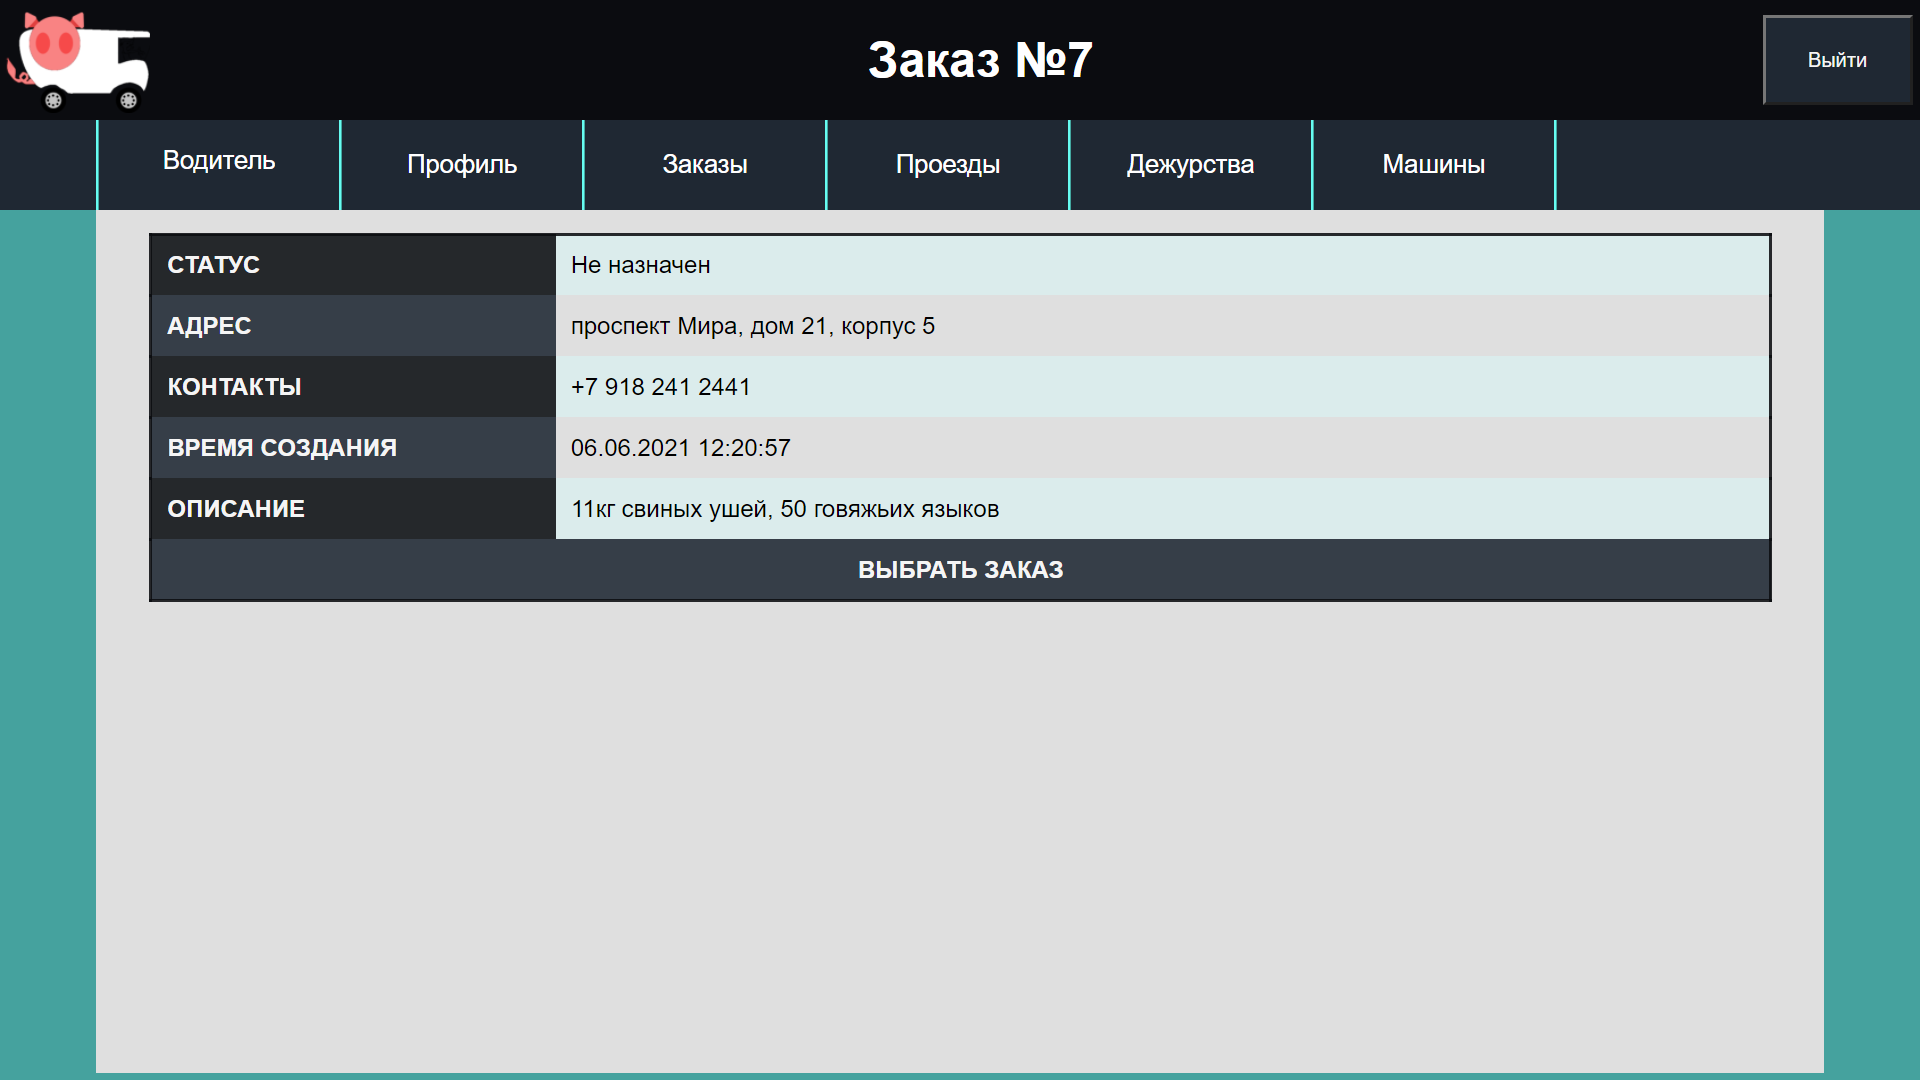
\includegraphics[scale=0.4, angle=0]{sc/pick_delivery}}
		\caption{Страница просмотра и выбора заказа (для роли водителя)}
		\label{pick_delivery_sc}
	\end{center}
\end{figure}

\begin{figure}[h!] 
	\begin{center}
		%		{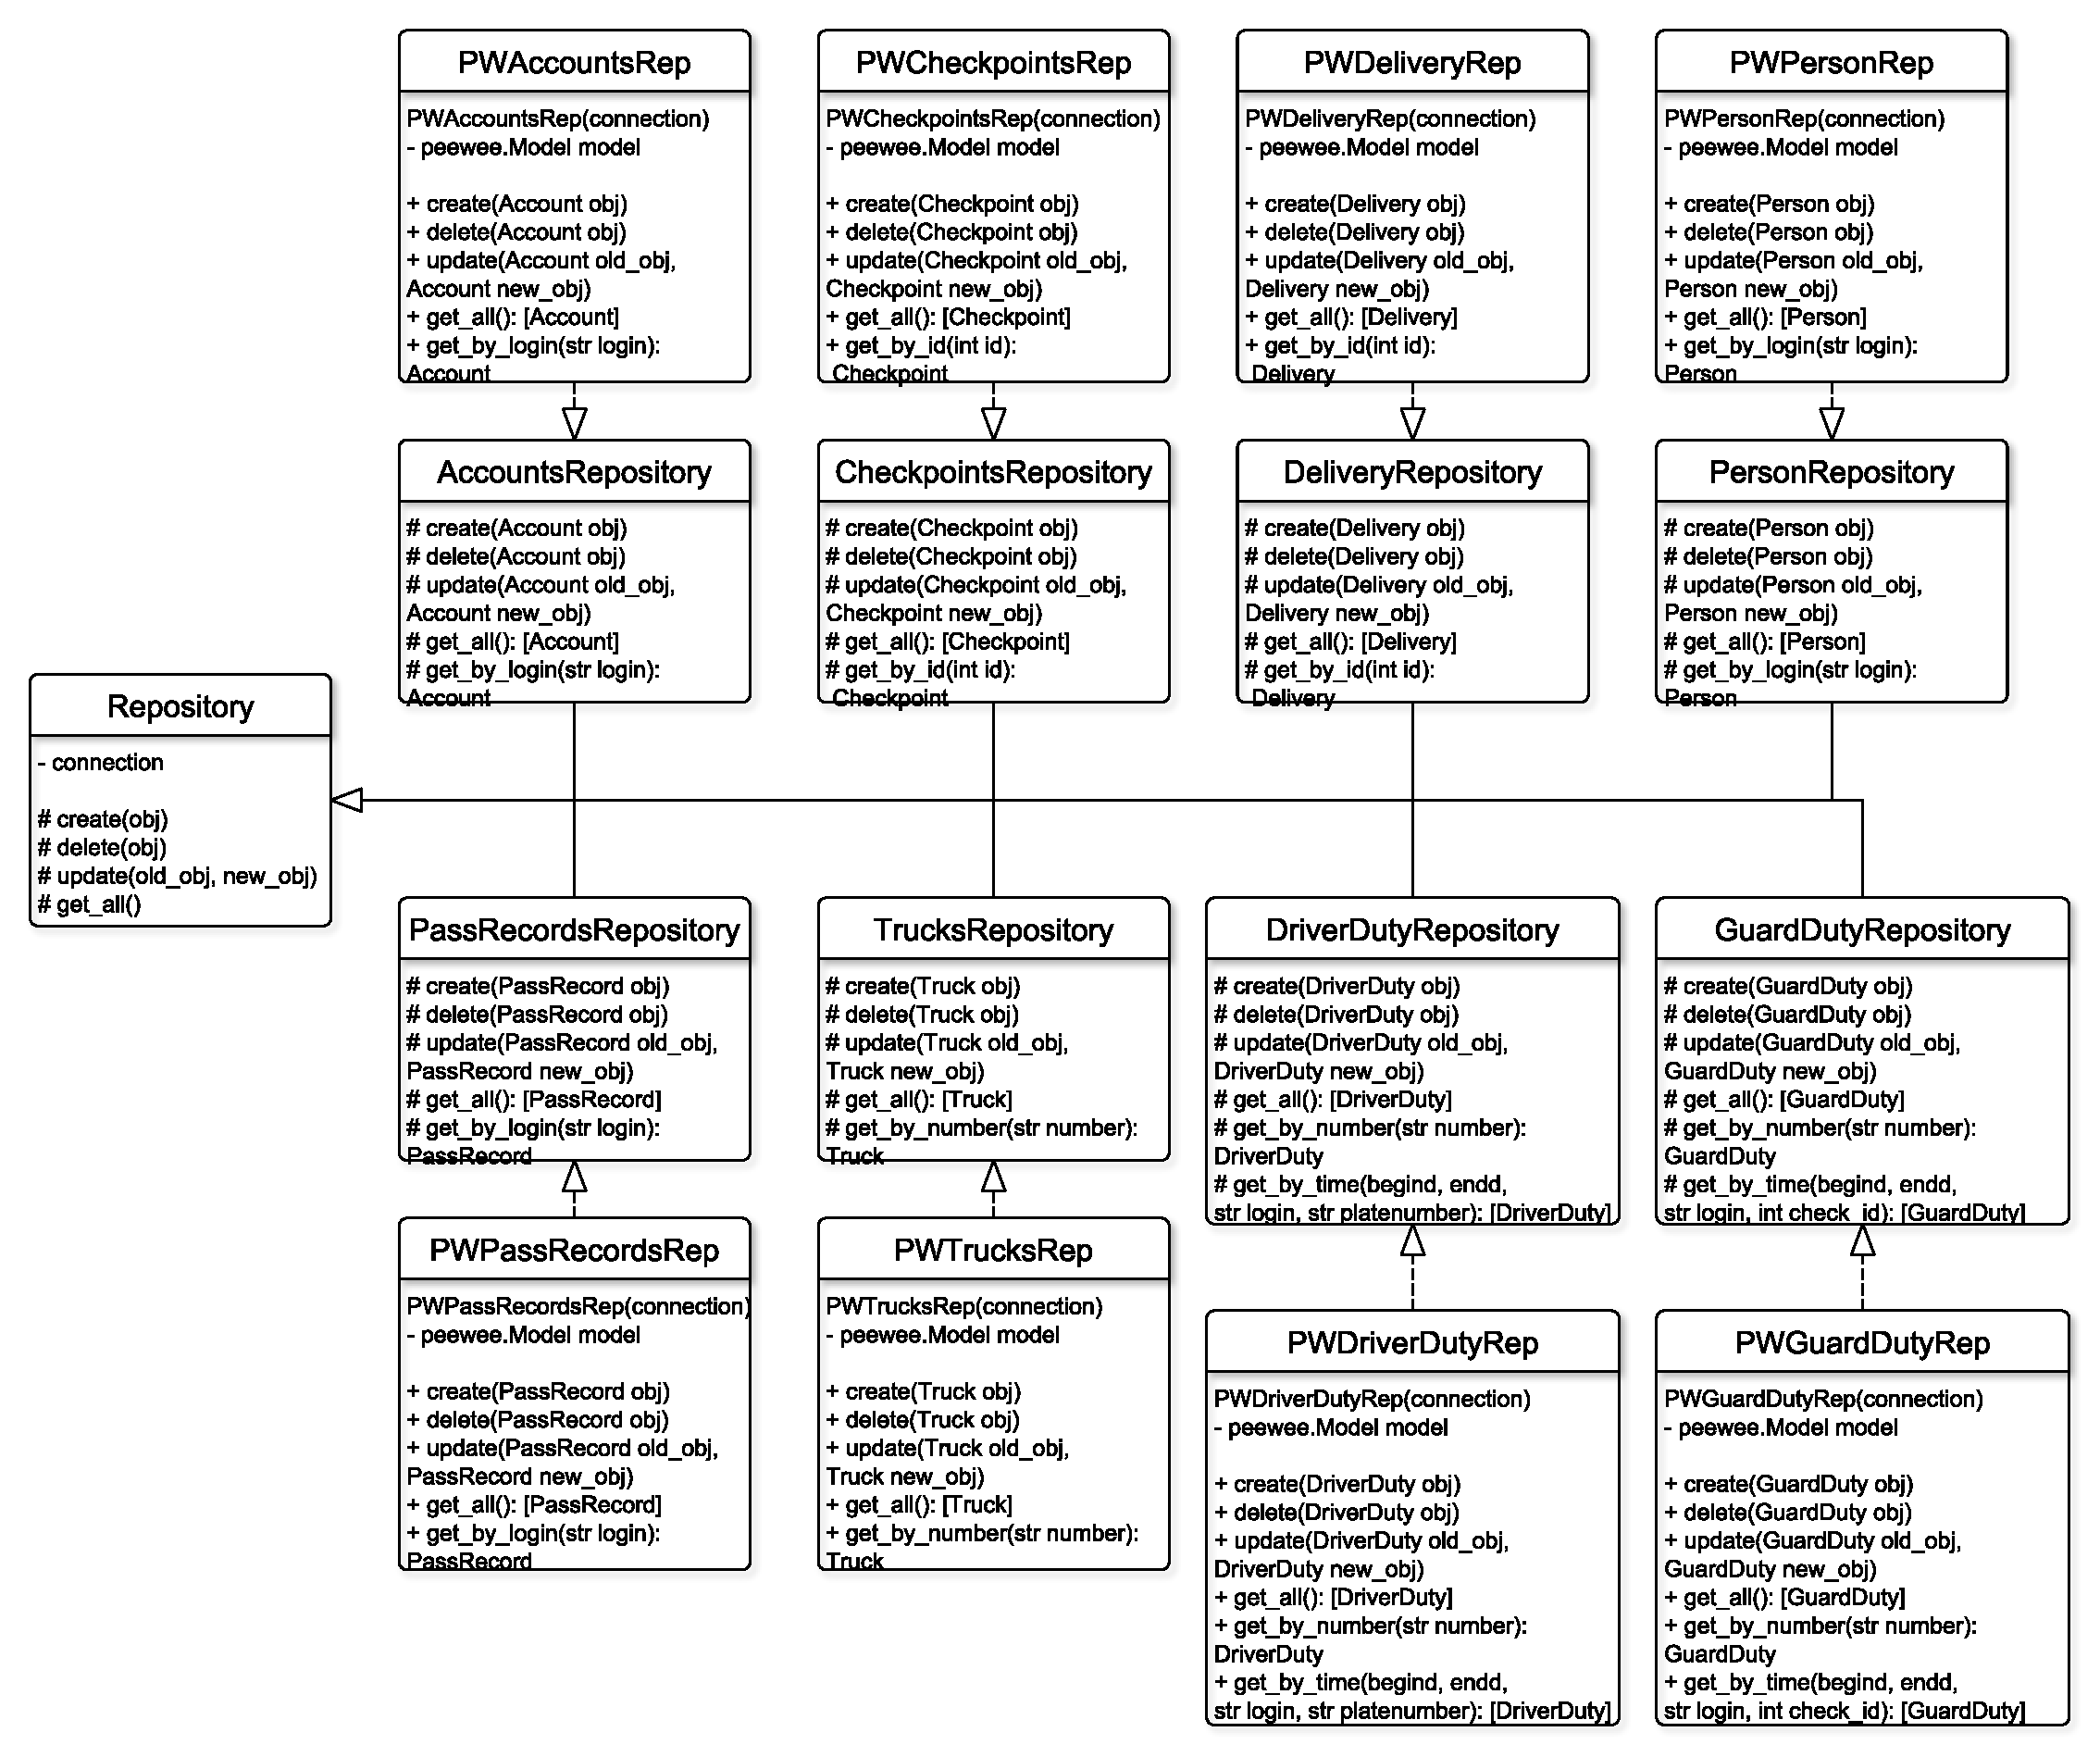
\includegraphics[height=14cm, width = 14cm]{uml/repsoitory.pdf}}
		{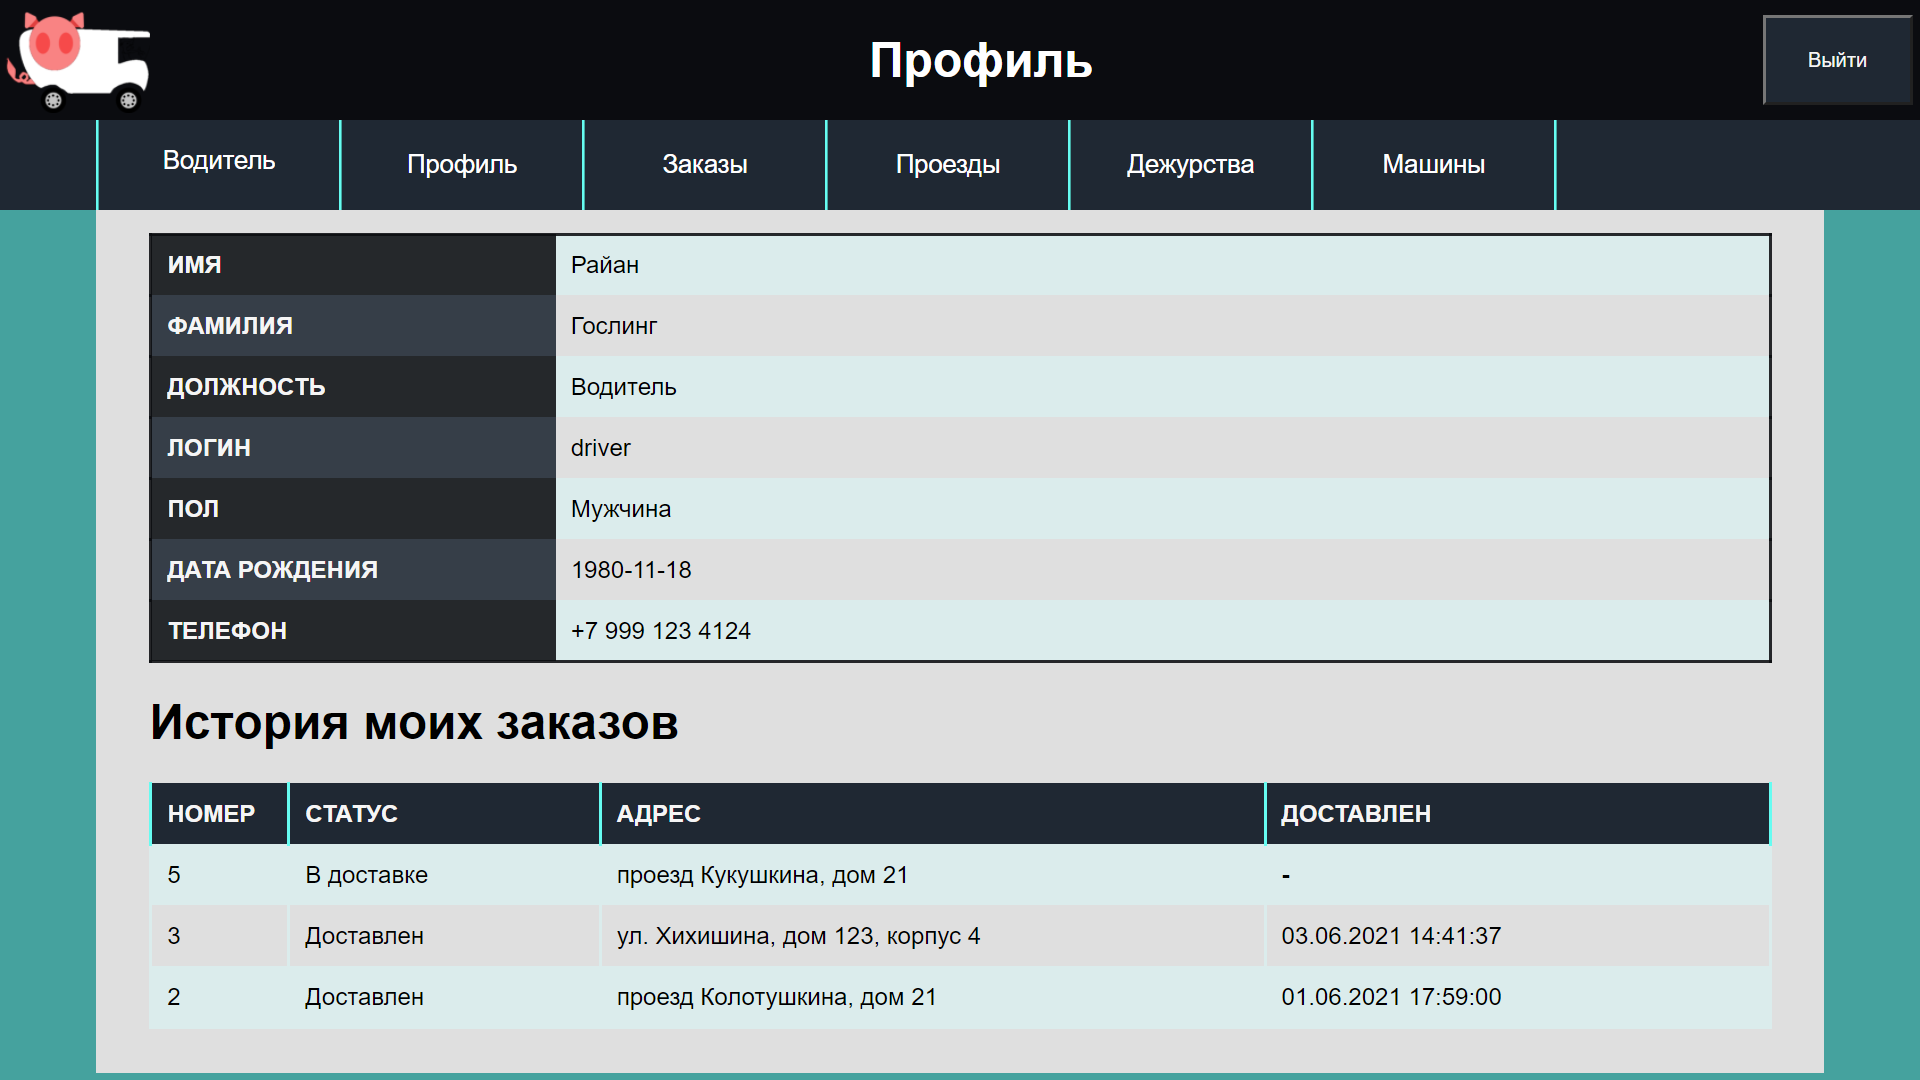
\includegraphics[scale=0.4, angle=0]{sc/driver_profile}}
		\caption{Личная страница (для роли водителя)}
		\label{driver_profile_sc}
	\end{center}
\end{figure}

\begin{figure}[h!] 
	\begin{center}
		%		{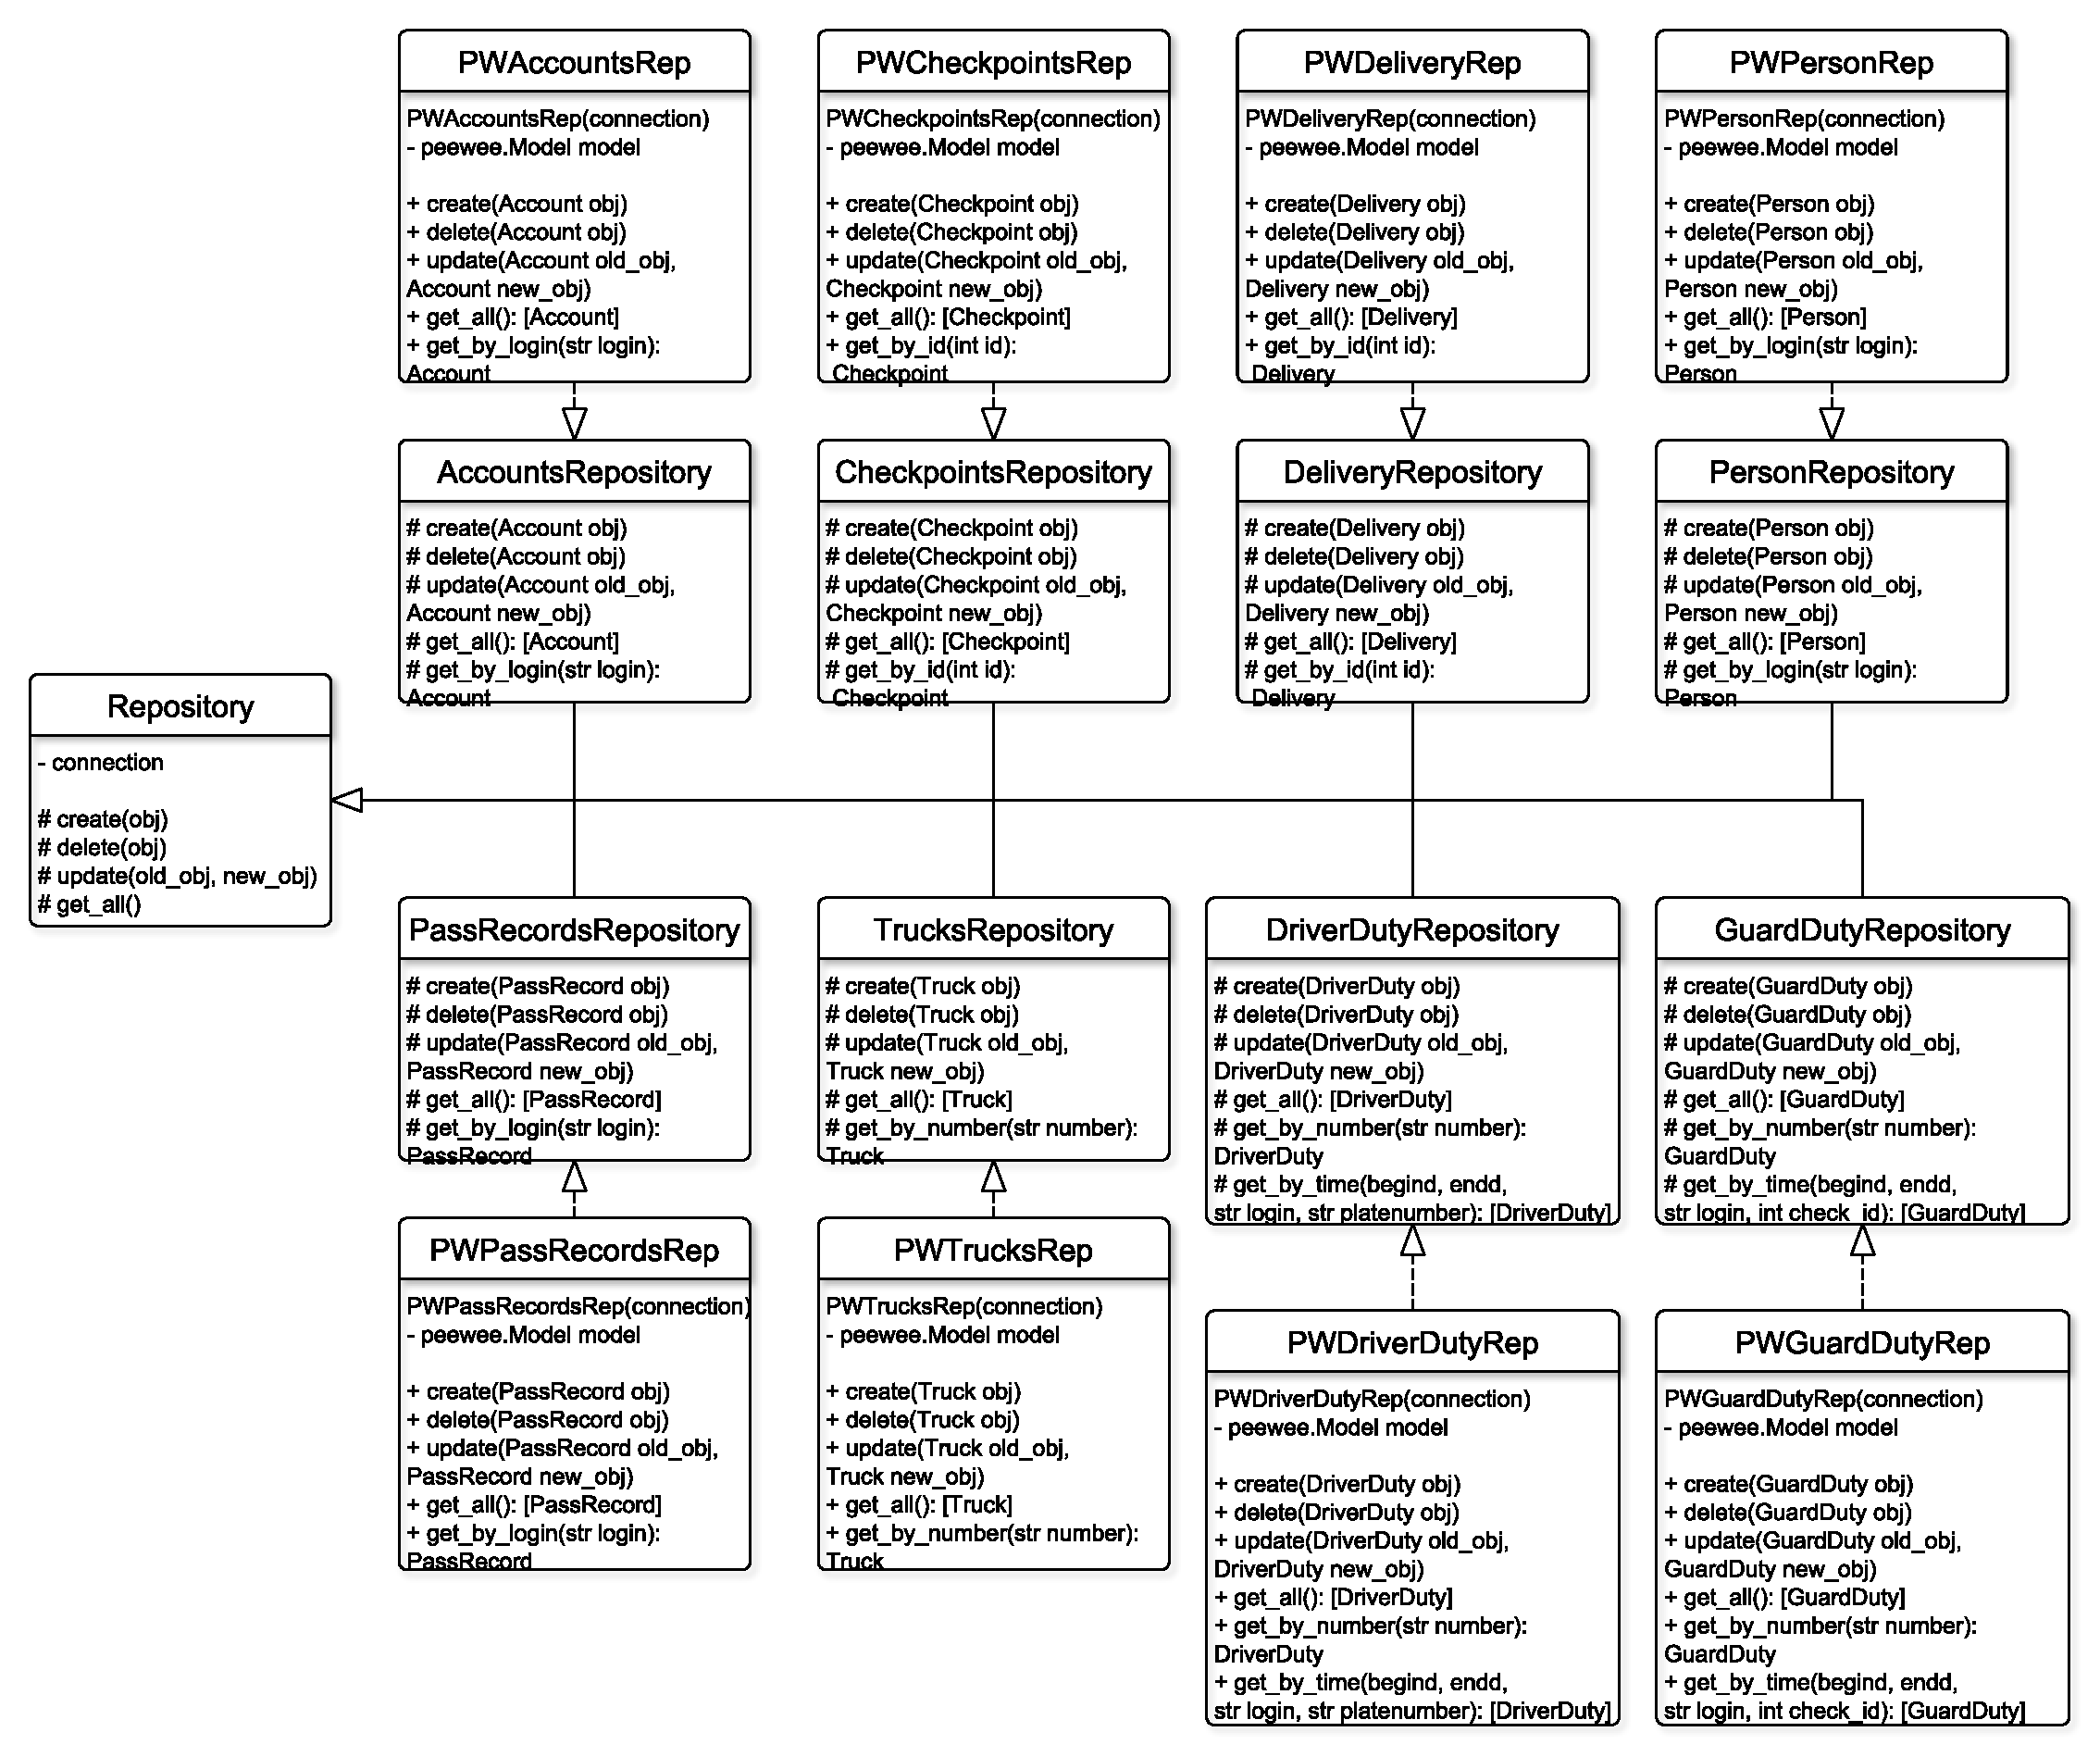
\includegraphics[height=14cm, width = 14cm]{uml/repsoitory.pdf}}
		{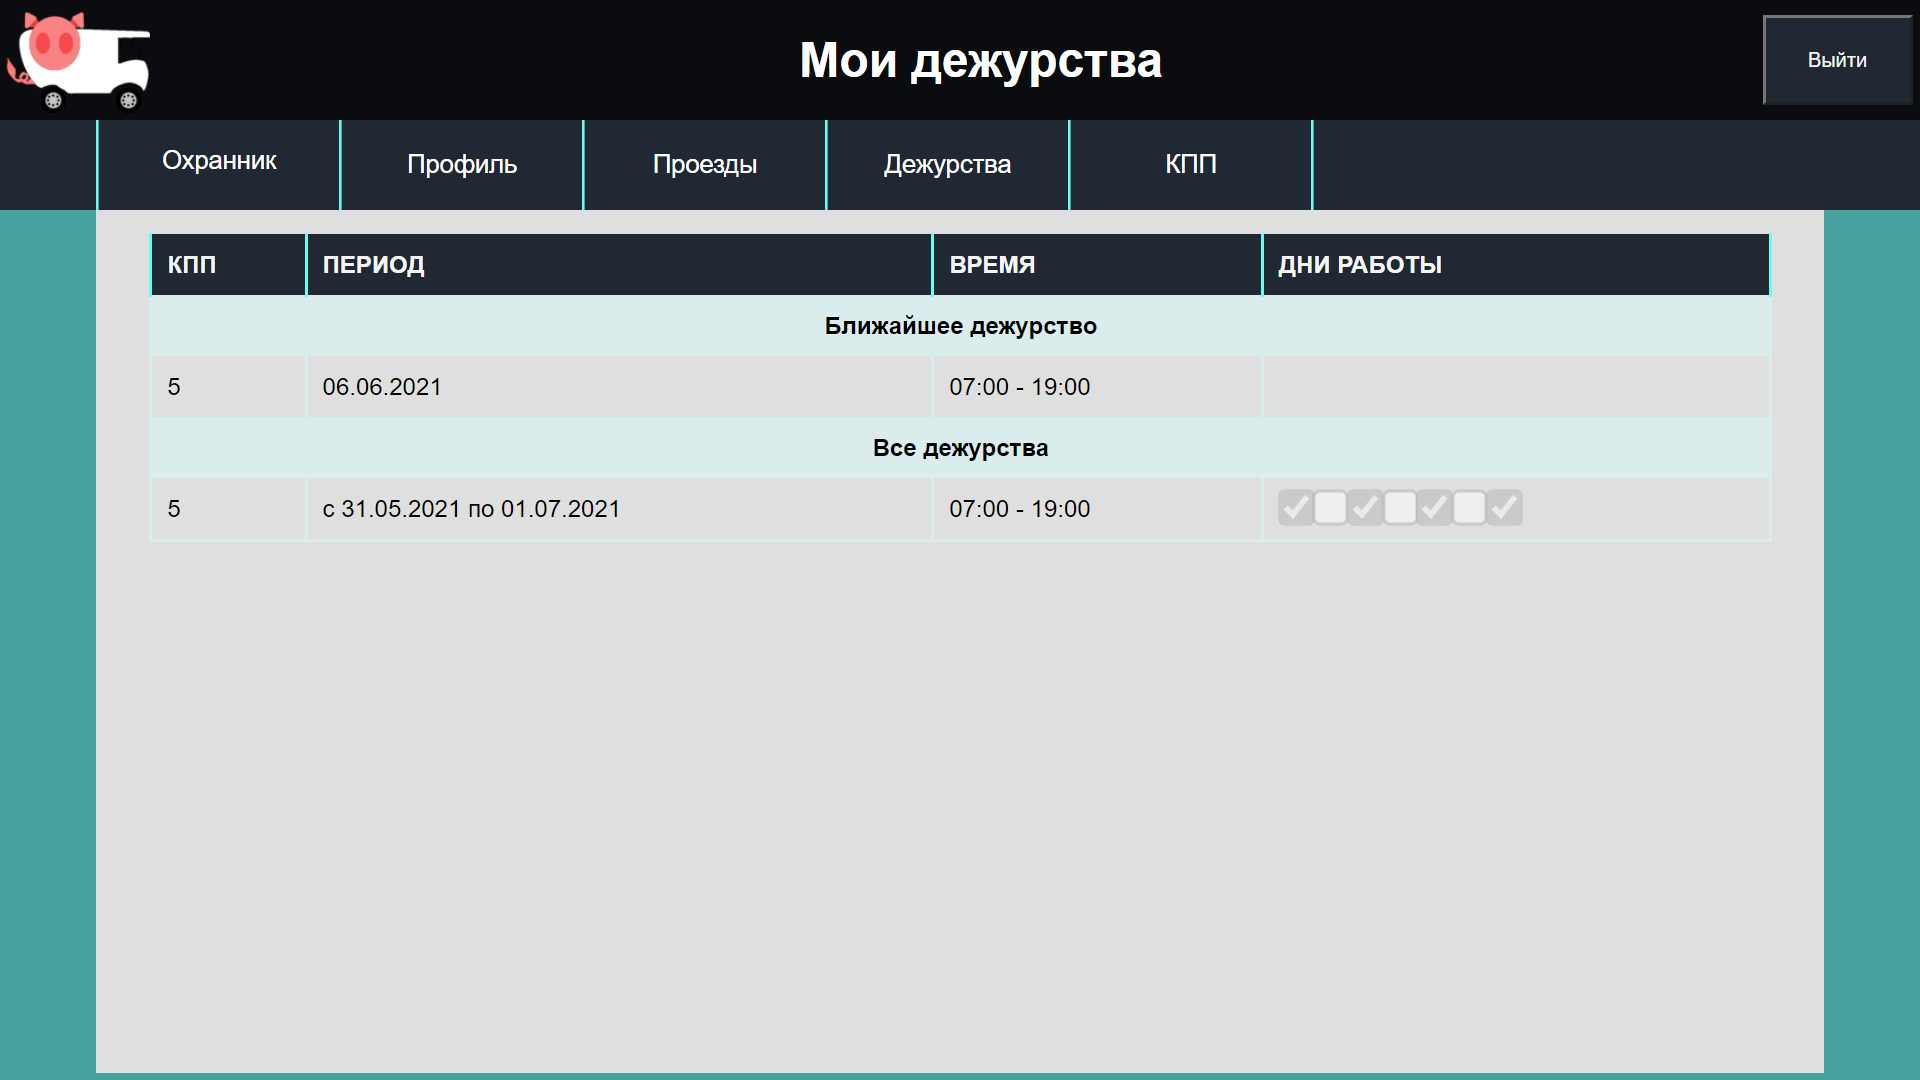
\includegraphics[scale=0.4, angle=0]{sc/guard_duty}}
		\caption{Страница просмотра дежурств (для роли охранника)}
		\label{guard_duty_sc}
	\end{center}
\end{figure}

\begin{figure}[h!] 
	\begin{center}
		%		{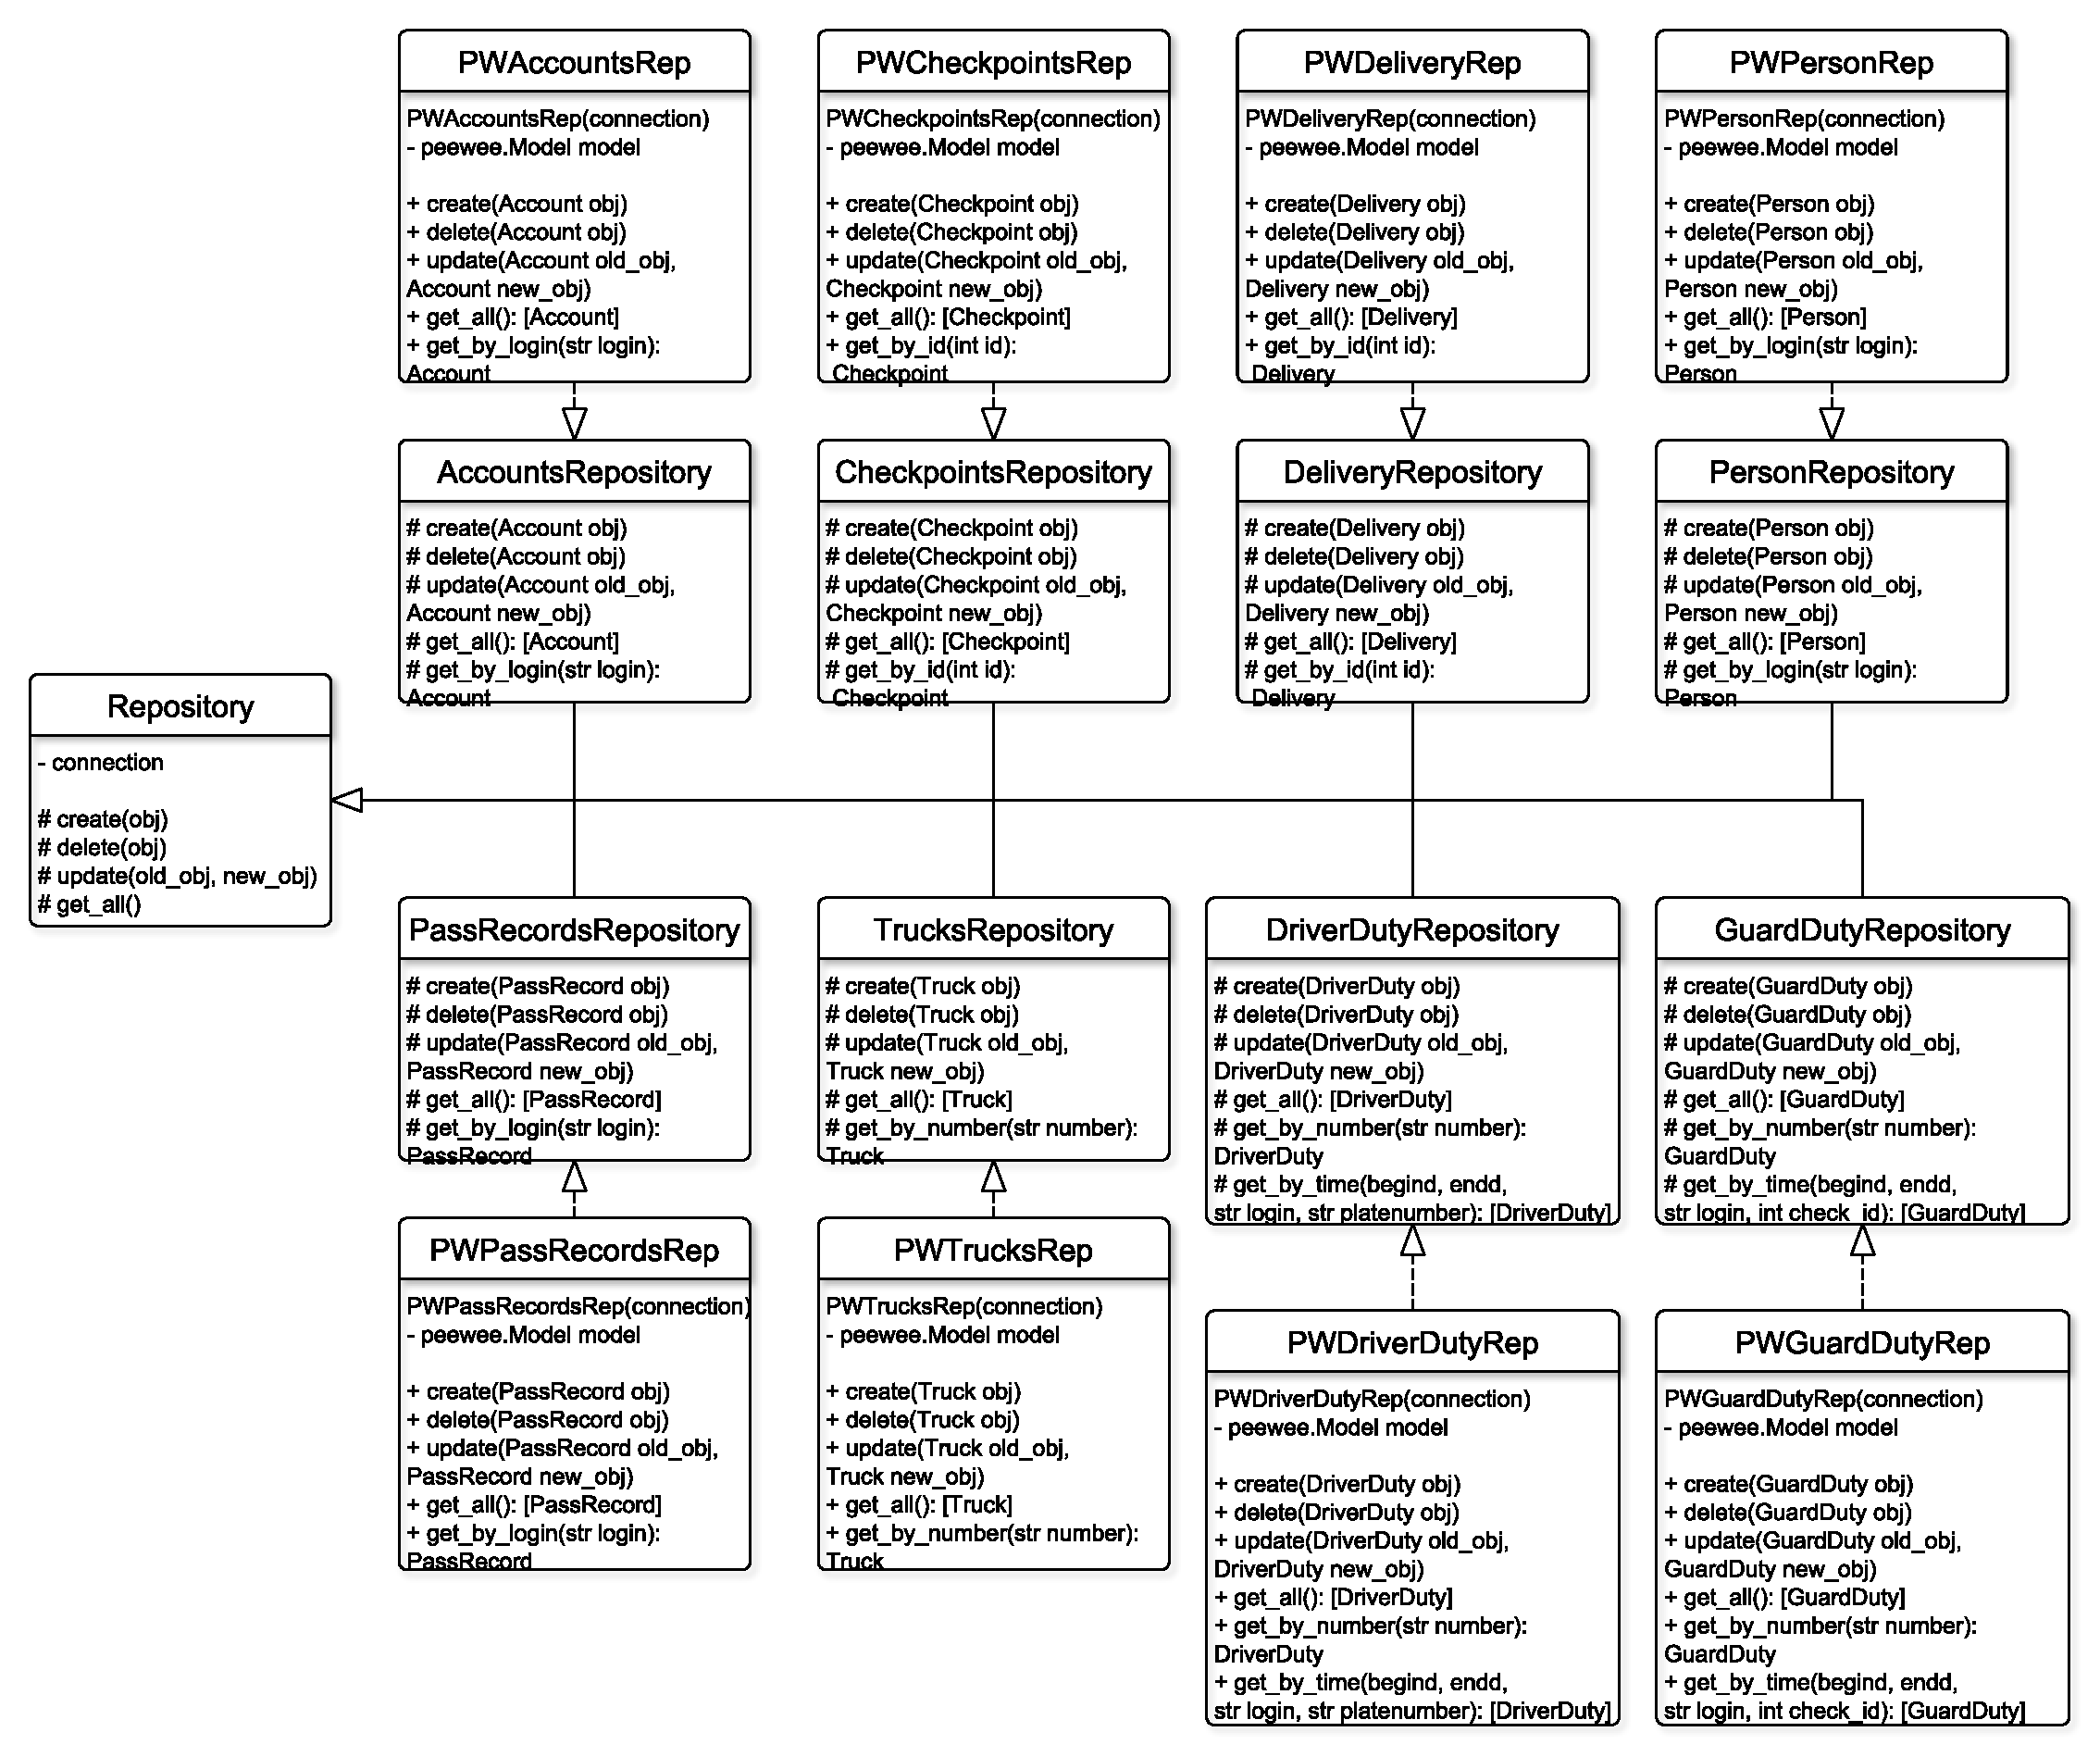
\includegraphics[height=14cm, width = 14cm]{uml/repsoitory.pdf}}
		{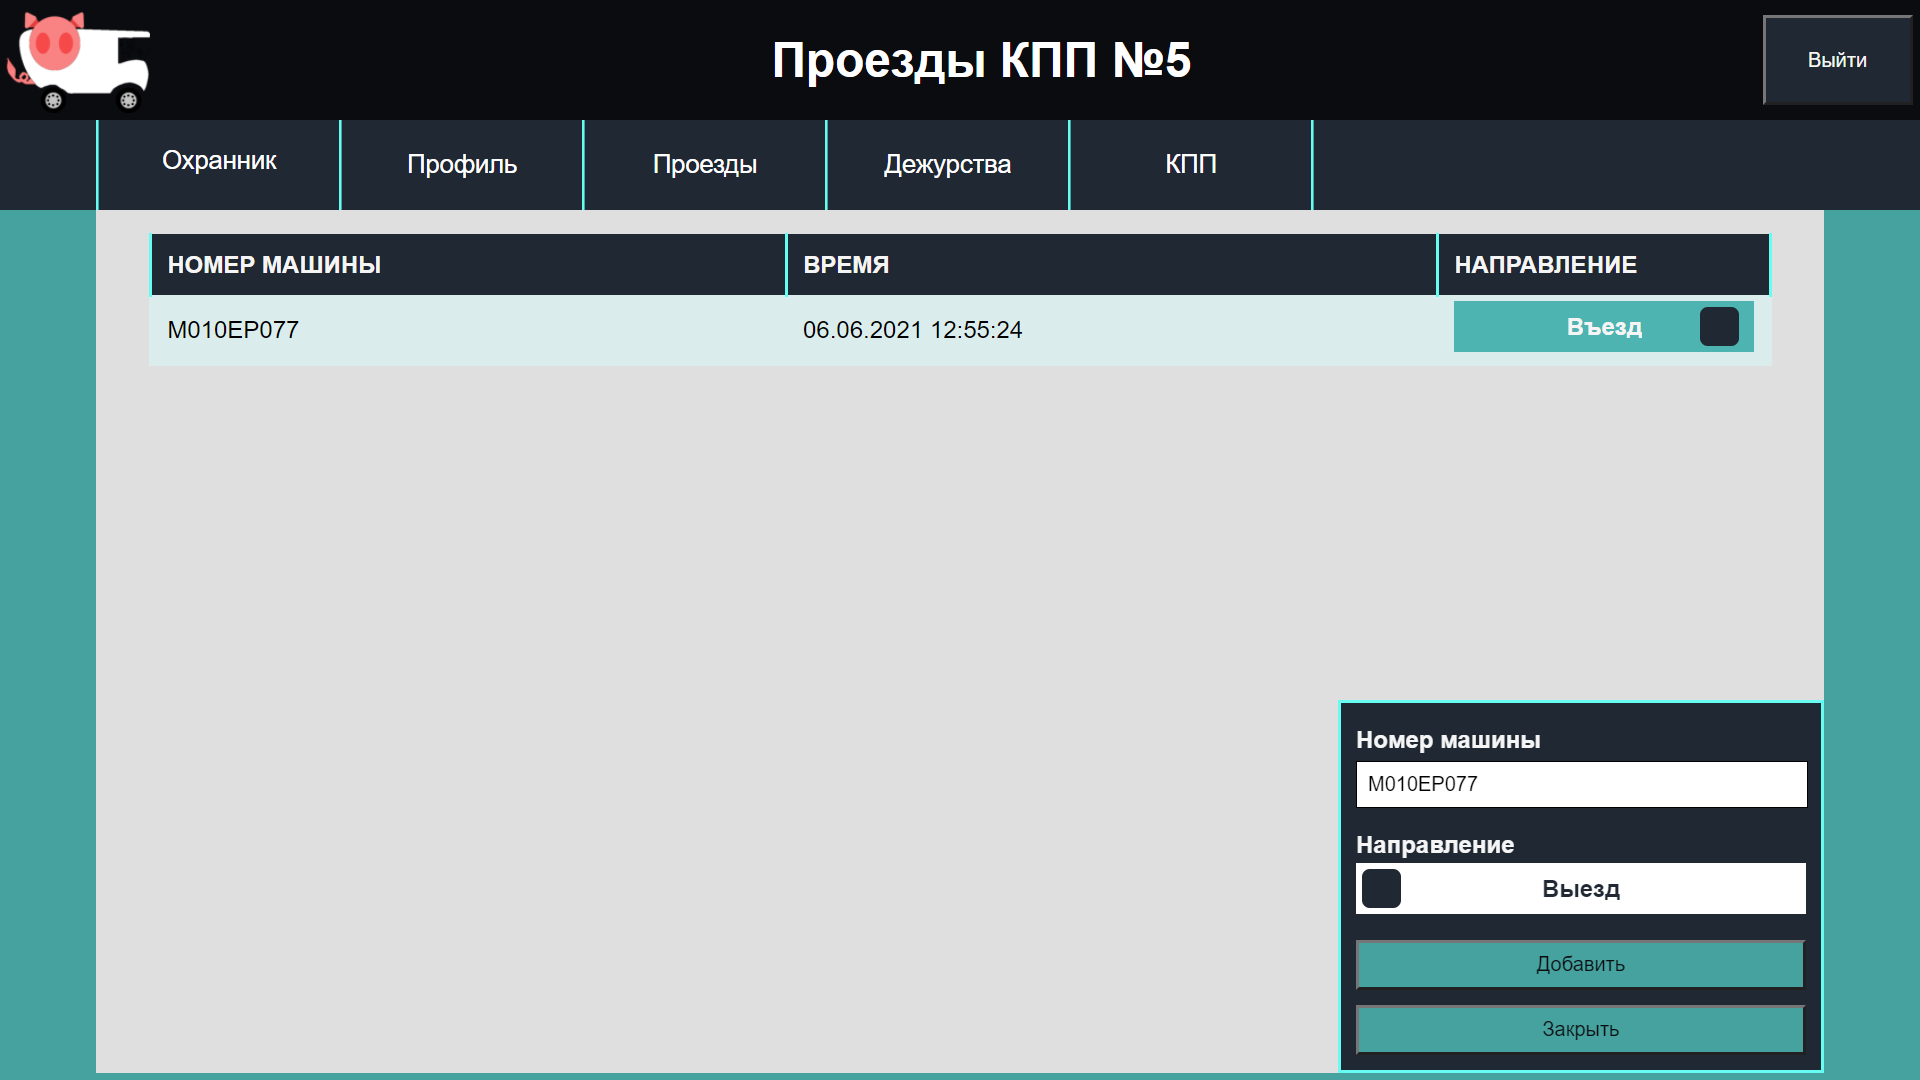
\includegraphics[scale=0.4, angle=0]{sc/pass_guard}}
		\caption{Страница просмотра и добавления записей проездов (для роли охранника)}
		\label{pass_guard_sc}
	\end{center}
\end{figure}

\newpage
Для неавторизованного пользователя доступны страницы входа в аккаунт и регистрации (рисунок \ref{login_sc} и \ref{signup_sc}) 

\begin{figure}[h!] 
	\begin{center}
		%		{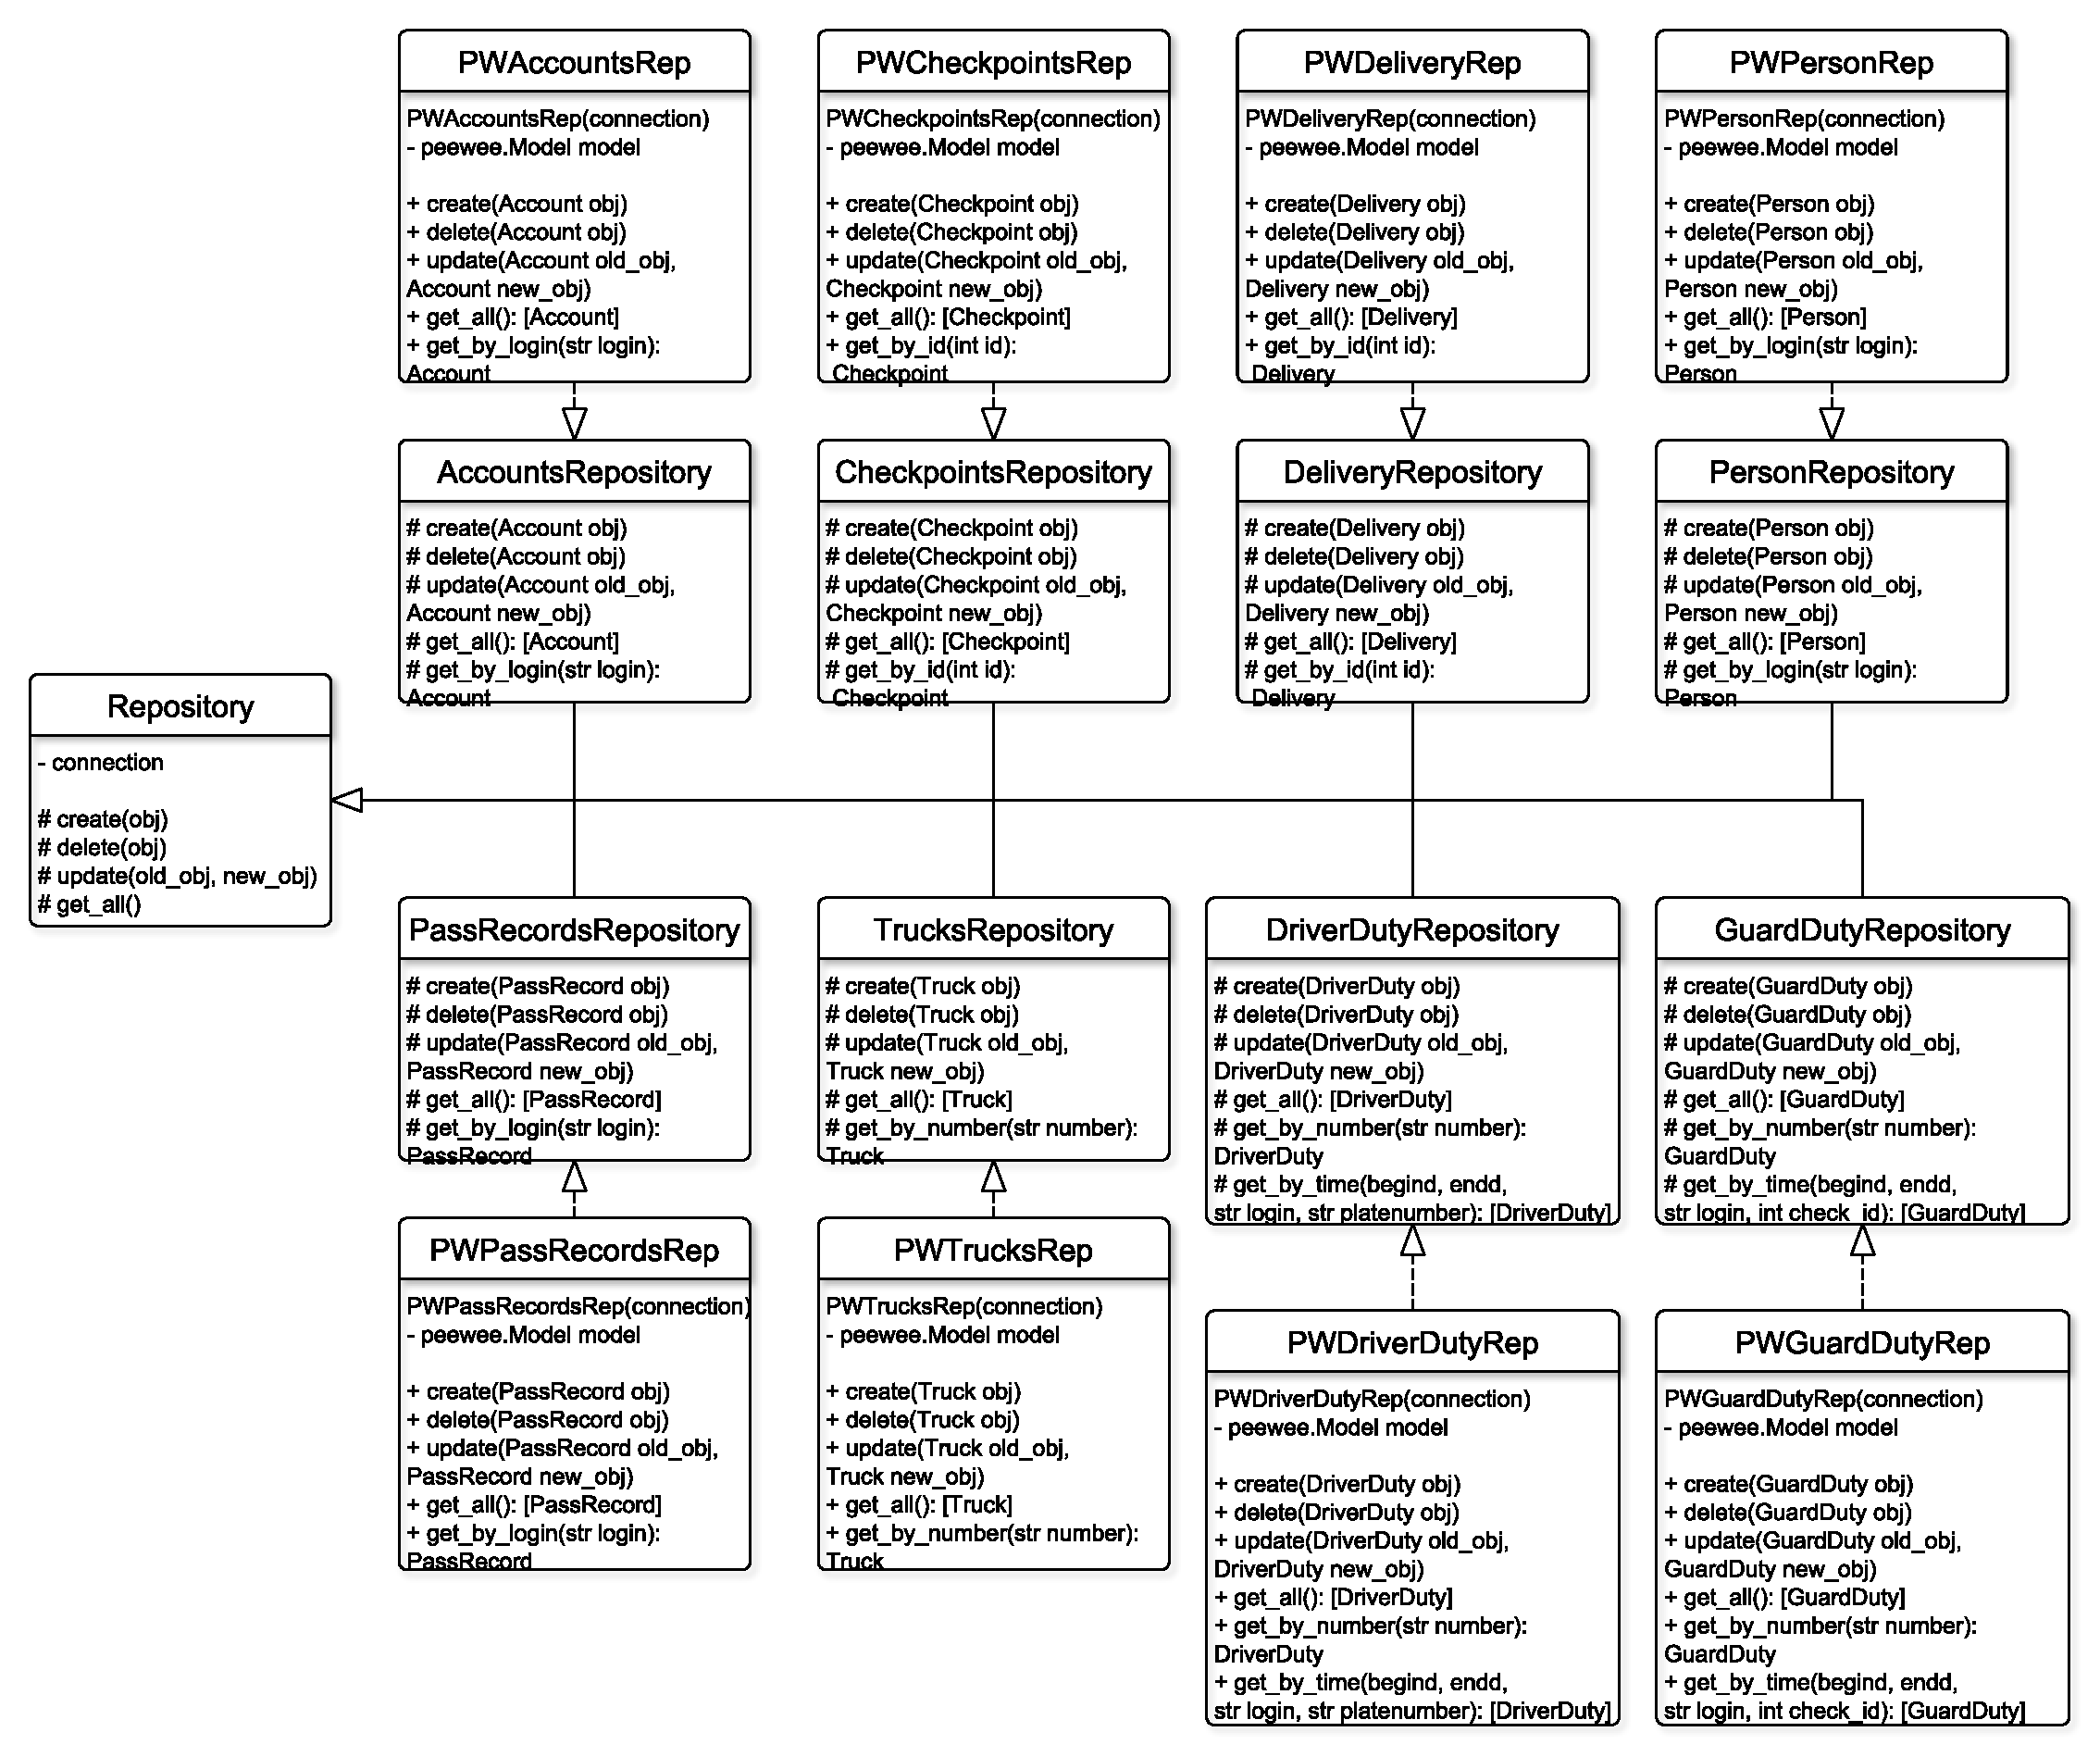
\includegraphics[height=14cm, width = 14cm]{uml/repsoitory.pdf}}
		{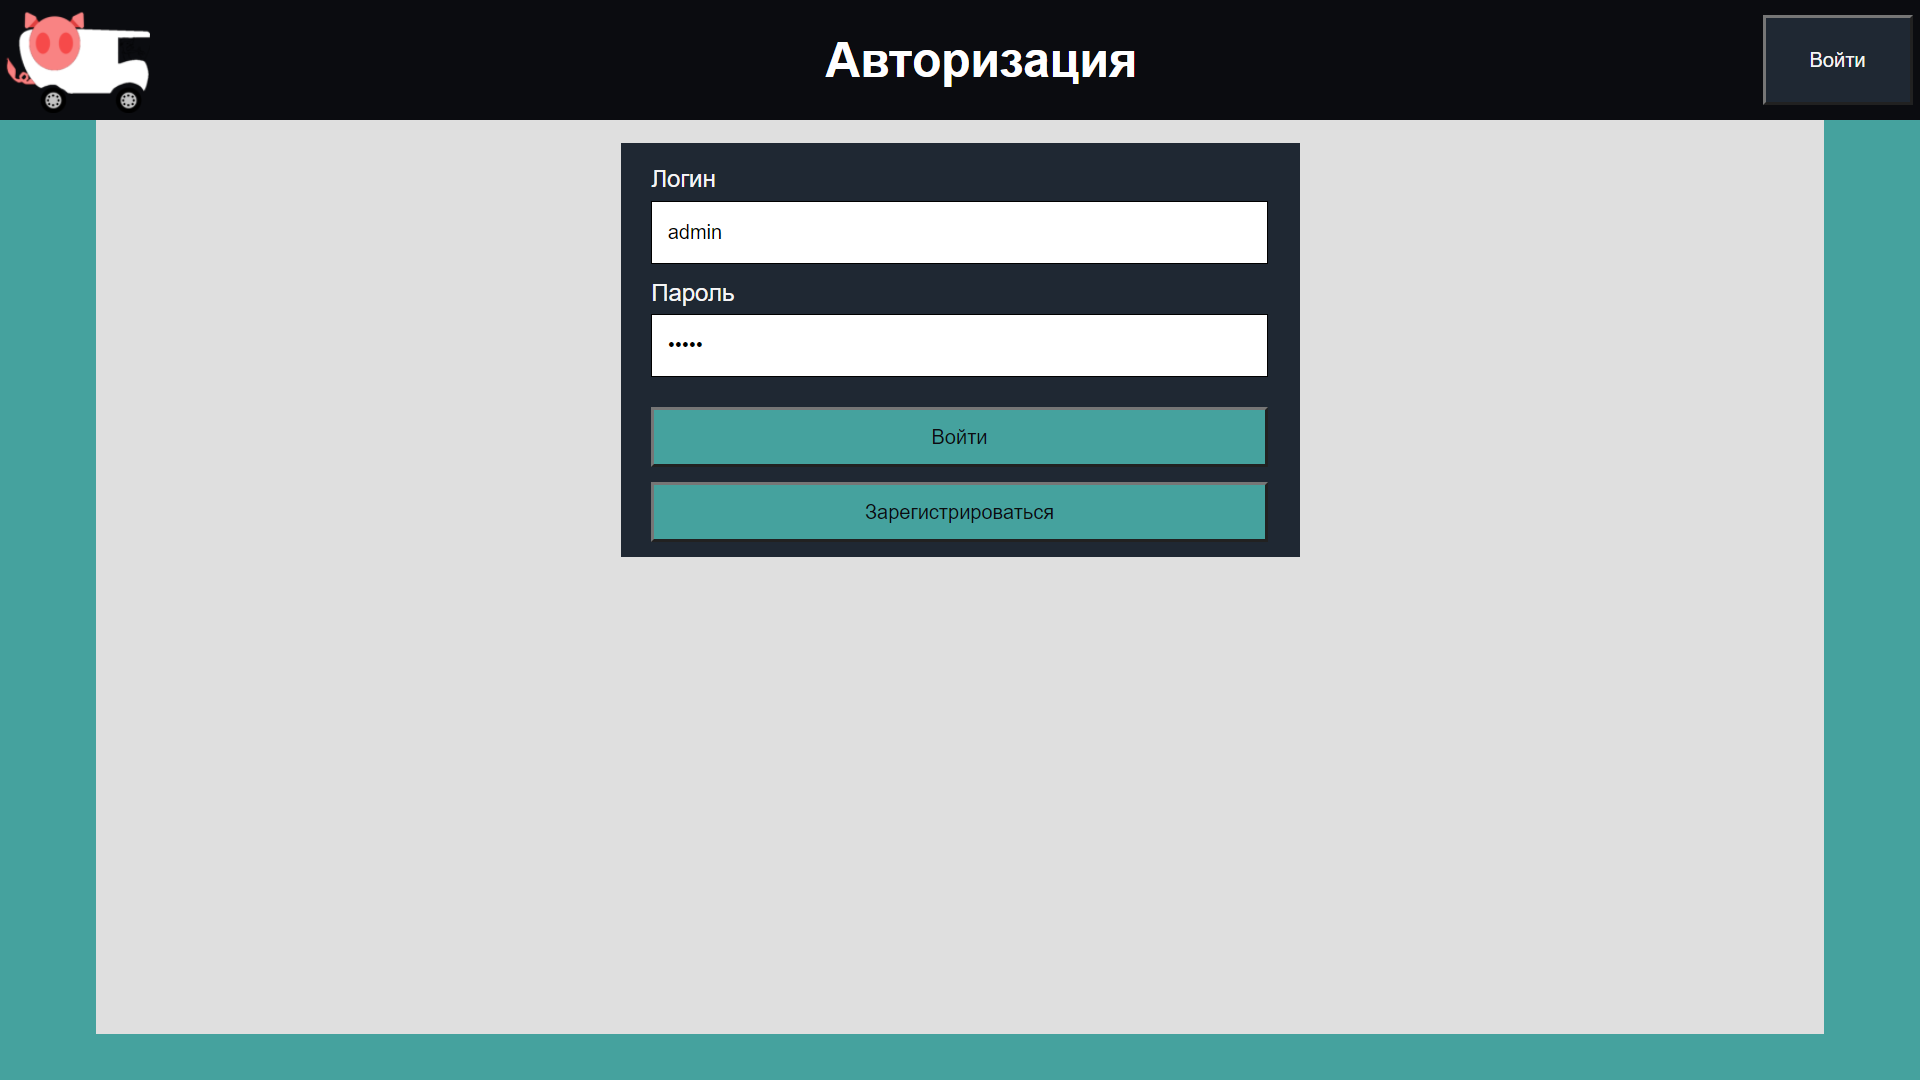
\includegraphics[scale=0.38, angle=0]{sc/login}}
		\caption{Страница авторизации}
		\label{login_sc}
	\end{center}
\end{figure}

\begin{figure}[h!] 
	\begin{center}
		%		{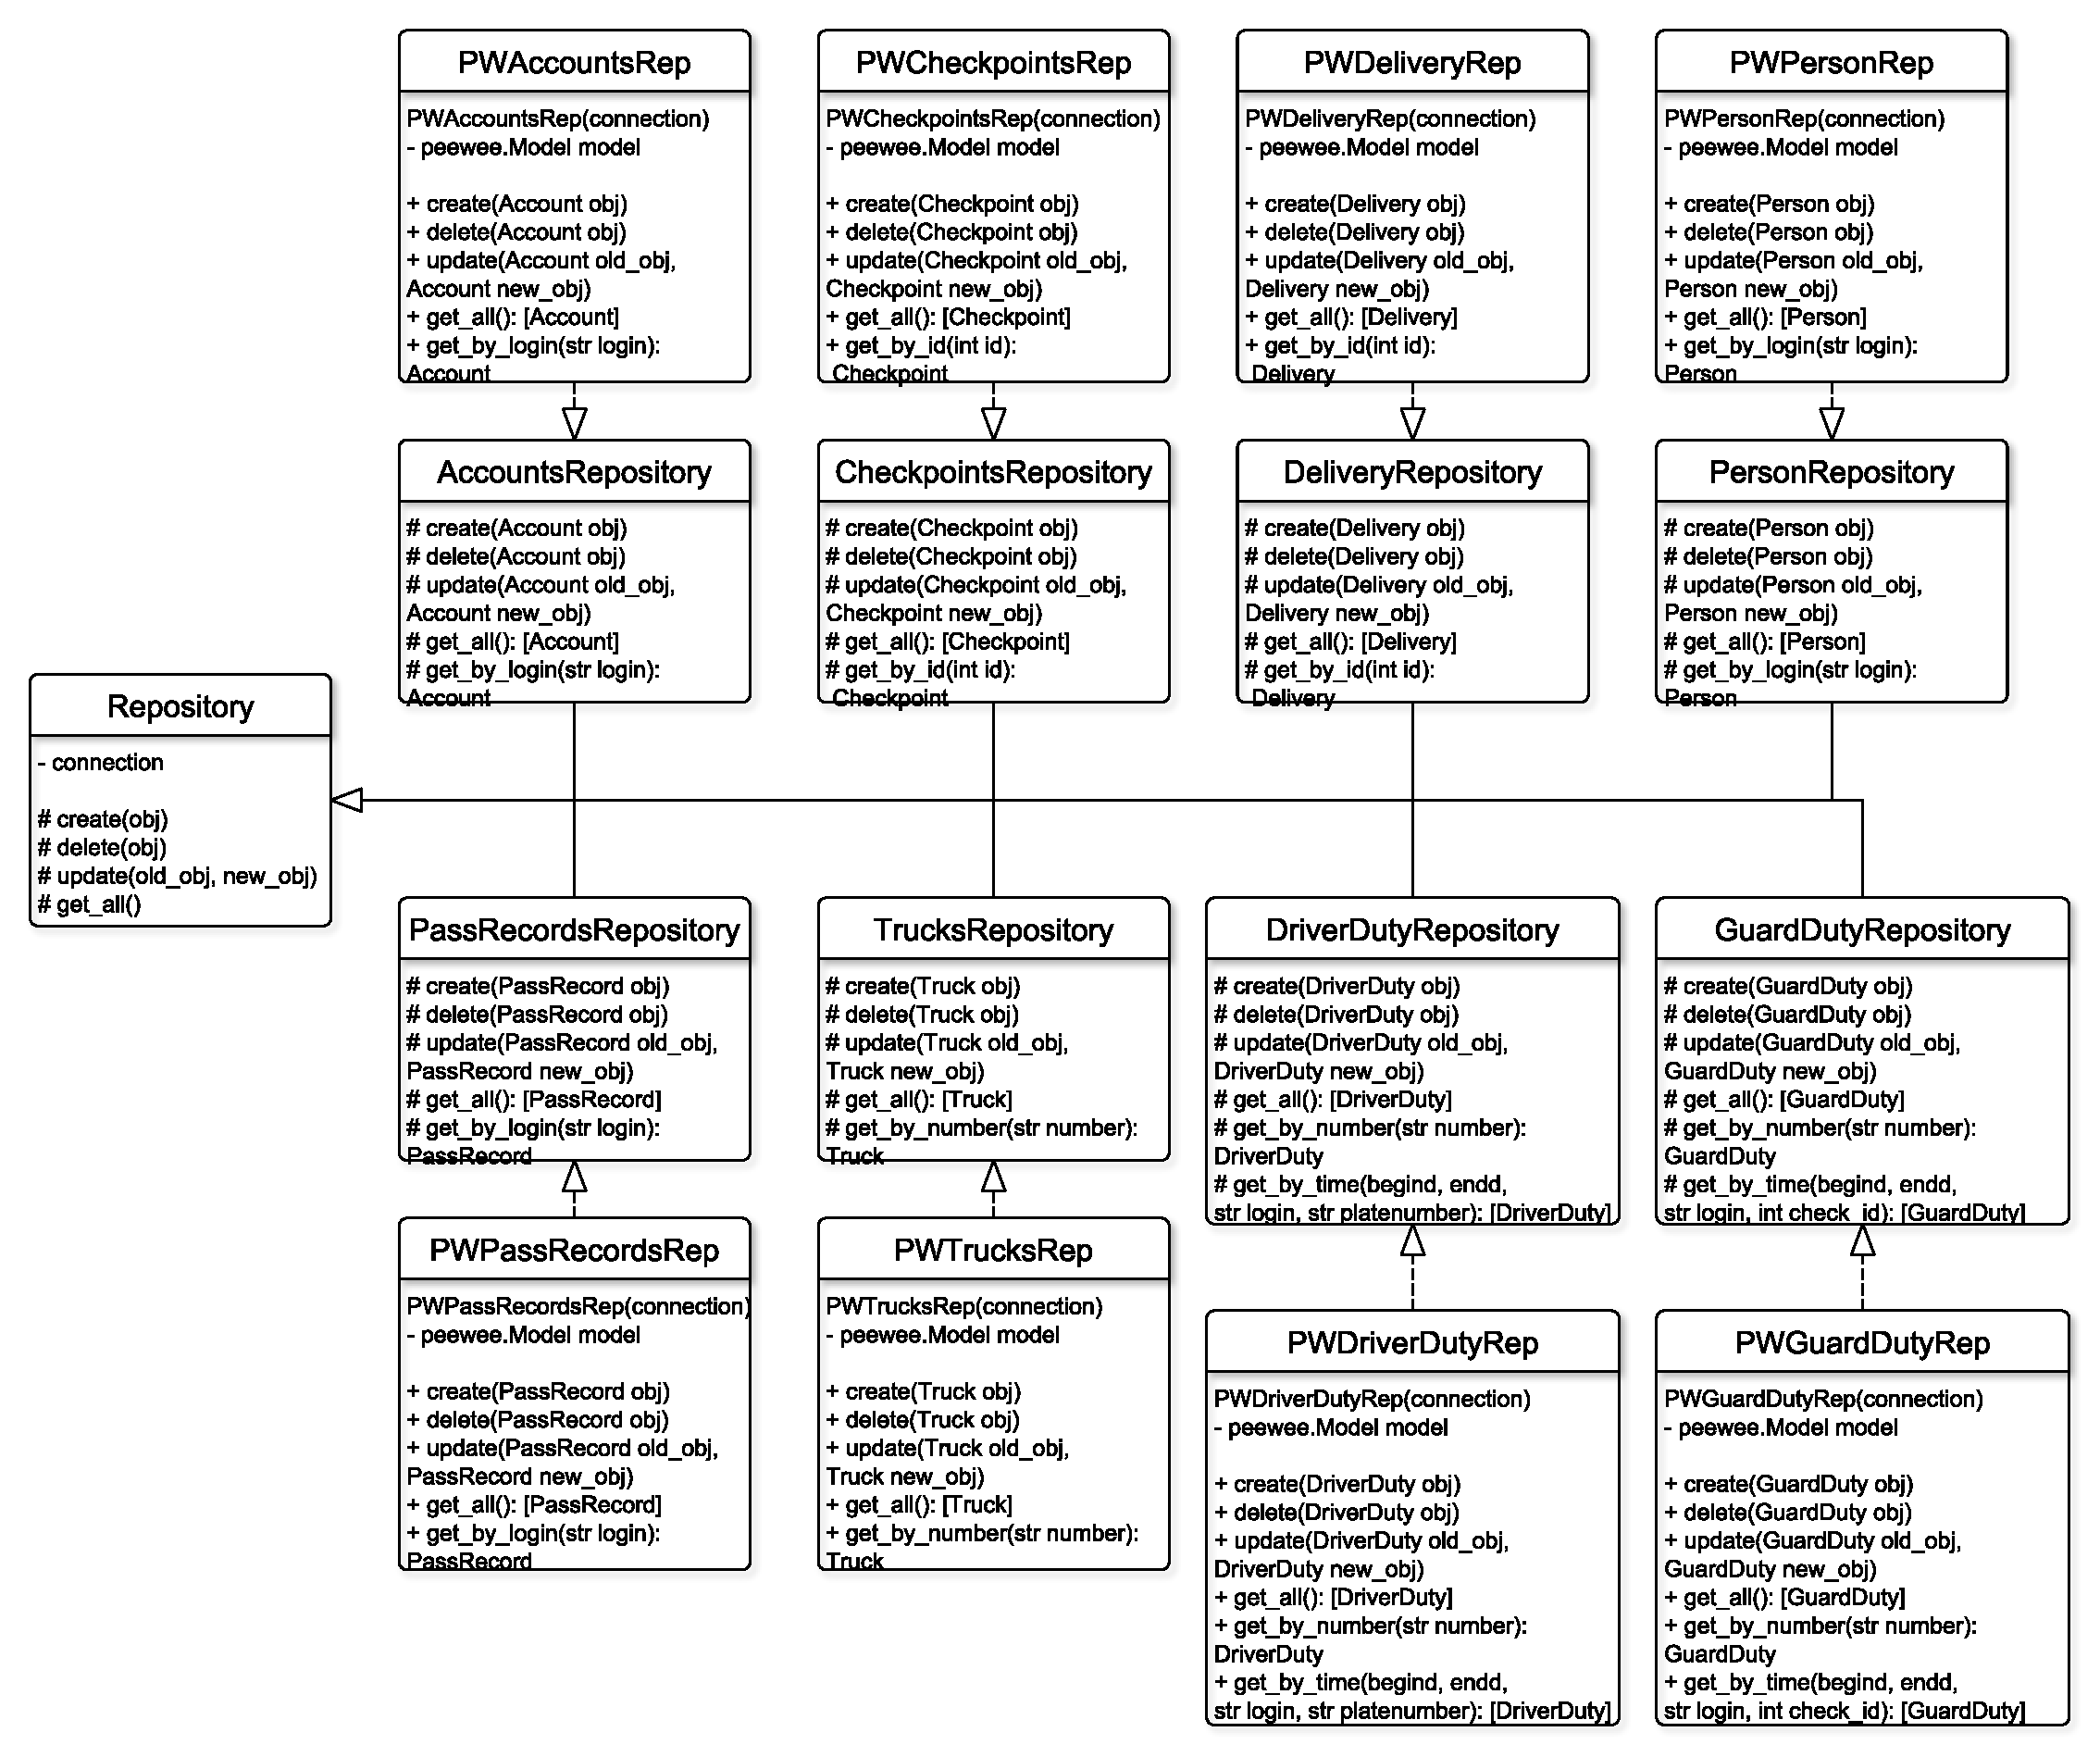
\includegraphics[height=14cm, width = 14cm]{uml/repsoitory.pdf}}
		{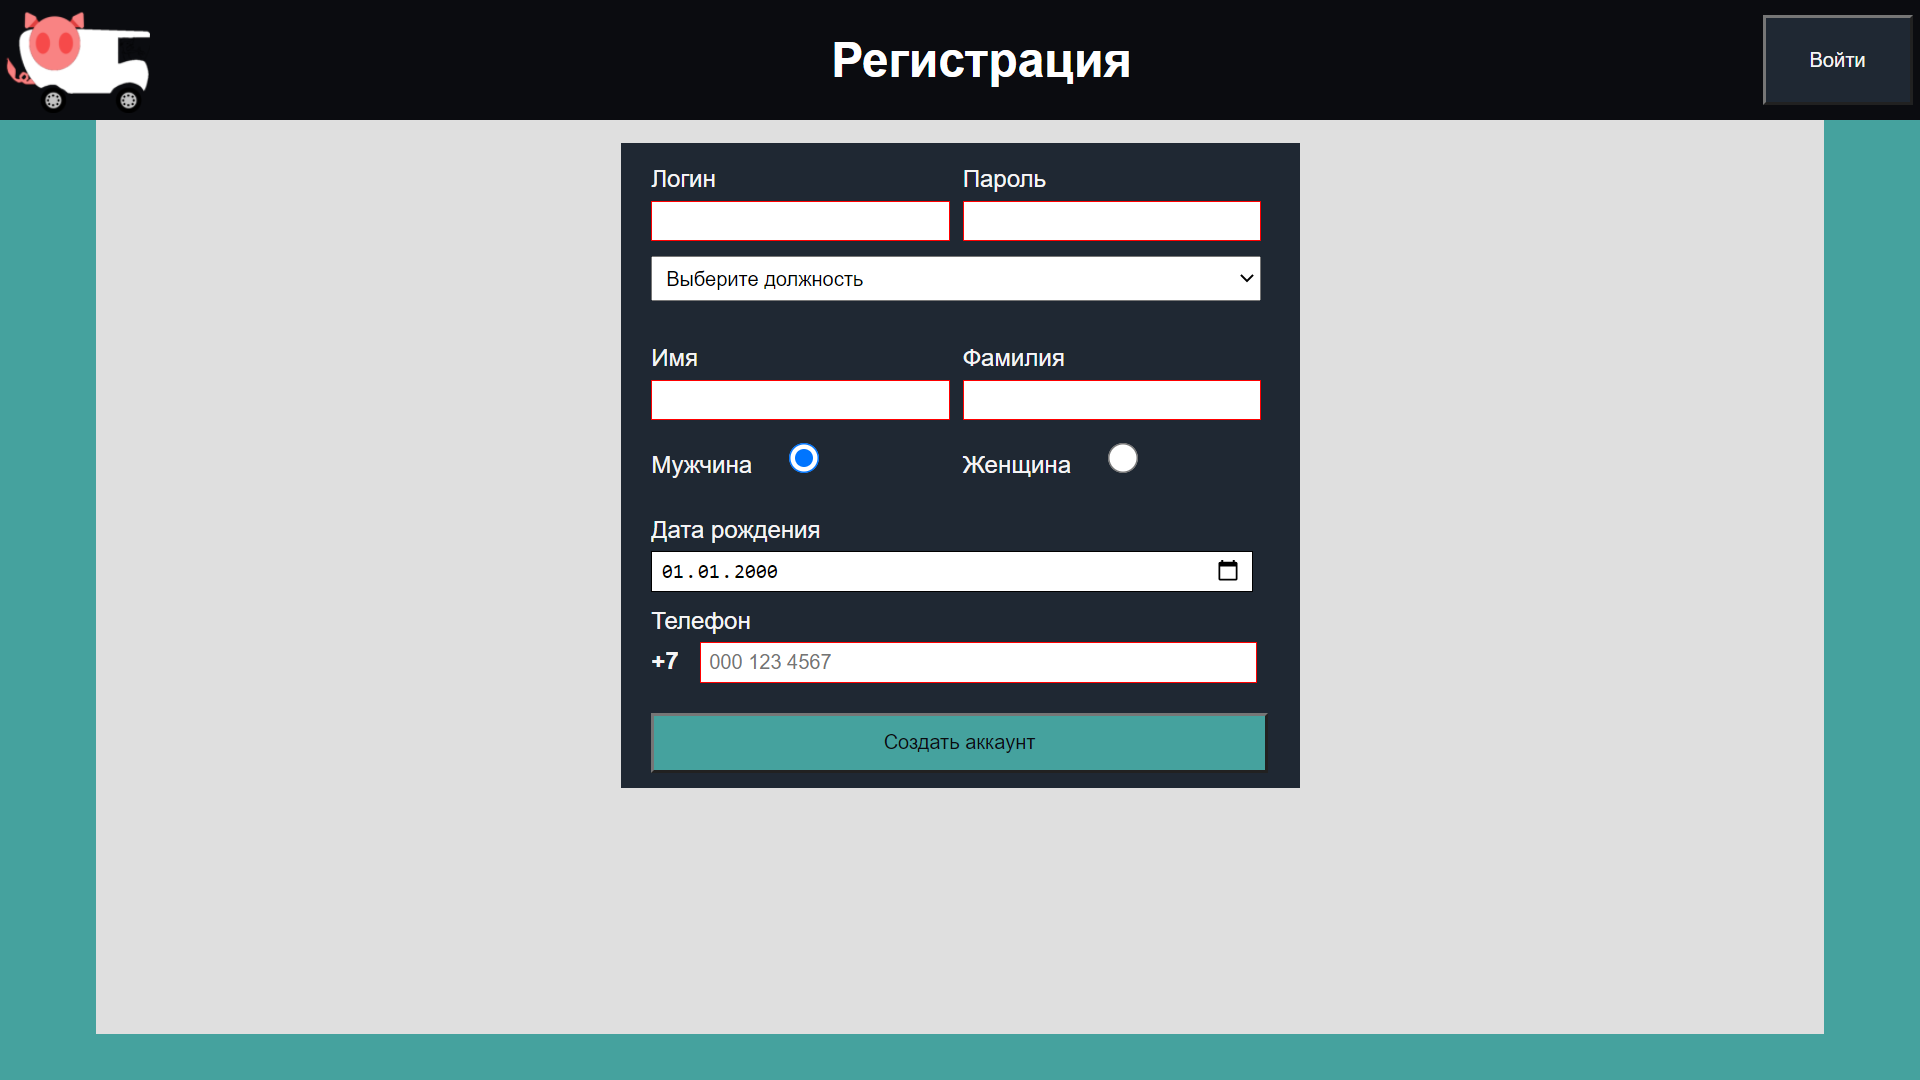
\includegraphics[scale=0.38, angle=0]{sc/signup}}
		\caption{Страница регистрации}
		\label{signup_sc}
	\end{center}
\end{figure}


\section*{Вывод}
Результатом технологической части стал выбор средств программной реализации, реализация и описание структуры базы данных и приложения, визуальная демонстрация интерфейса приложения.
